% **************************************************************************************************************
% A Classic Thesis Style
% An Homage to The Elements of Typographic Style
%
% Copyright (C) 2015 André Miede http://www.miede.de
%
% License:
% This program is free software; you can redistribute it and/or modify
% it under the terms of the GNU General Public License as published by
% the Free Software Foundation; either version 2 of the License, or
% (at your option) any later version.
%
% This program is distributed in the hope that it will be useful,
% but WITHOUT ANY WARRANTY; without even the implied warranty of
% MERCHANTABILITY or FITNESS FOR A PARTICULAR PURPOSE.  See the
% GNU General Public License for more details.
%
% You should have received a copy of the GNU General Public License
% along with this program; see the file COPYING.  If not, write to
% the Free Software Foundation, Inc., 59 Temple Place - Suite 330,
% Boston, MA 02111-1307, USA.
%
% **************************************************************************************************************
\RequirePackage{fix-cm} % fix some latex issues see: http://texdoc.net/texmf-dist/doc/latex/base/fixltx2e.pdf
\documentclass[ twoside,openright,titlepage,numbers=noenddot,headinclude,%1headlines,% letterpaper a4paper
                footinclude=true,cleardoublepage=empty,abstractoff, % <--- obsolete, remove (todo)
                BCOR=5mm,paper=a4,fontsize=11pt,%11pt,a4paper,%
                francais,ngerman,american,%
                ]{scrreprt}

%********************************************************************
% Note: Make all your adjustments in here
%*******************************************************
\input{classicthesis-config}

%********************************************************************
% Bibliographies
%*******************************************************
\addbibresource{Bibliography.bib}
\addbibresource[label=ownpubs]{lafay_Publications.bib}

%********************************************************************
% Hyphenation
%*******************************************************
%\hyphenation{put special hyphenation here}
%*******************************************************
\begin{document}
\frenchspacing
\raggedbottom
\selectlanguage{francais} % american ngerman
%\renewcommand*{\bibname}{new name}
%\setbibpreamble{}
\pagenumbering{roman}
\pagestyle{plain}

% Frontmatter
%*******************************************************
\include{FrontBackmatter/DirtyTitlepage}
%*******************************************************
% Titlepage
%*******************************************************
\begin{titlepage}
    % if you want the titlepage to be centered, uncomment and fine-tune the line below (KOMA classes environment)
    \begin{addmargin}[-1cm]{-3cm}
    \begin{center}
        \large  

        \hfill

        \vfill

        \begingroup
            \color{Maroon}\spacedallcaps{\myTitle} \\ \bigskip
        \endgroup
		\medskip 
		\mySubtitle \\ \bigskip

		\vfill
		
        \includegraphics[scale=.3]{gfx/title/citySound}\footnote{d'après http://www.joesdaily.com/art-design/your-words-turned-into-art/} \\ \medskip
		
		\vfill
		
        \spacedlowsmallcaps{\myName}

        \vfill
        
        \myDegree \\ \bigskip
        
        \myDepartment \\                            
        \myFaculty \\
        \myUni , \myLocation\\ \bigskip
		
		\vfill 
		
        \myTime 

        \vfill                      

    \end{center}  
  \end{addmargin}       
\end{titlepage}   
\include{FrontBackmatter/Titleback}
\cleardoublepage%*******************************************************
% Dedication
%*******************************************************
\thispagestyle{empty}
%\phantomsection 
\refstepcounter{dummy}
\pdfbookmark[1]{Dédicace}{Dédicace}

\vspace*{3cm}

\medskip

\begin{center}
\textit{À ma famille.}
\end{center}
%\cleardoublepage\include{FrontBackmatter/Foreword}
\cleardoublepage%*******************************************************
% Abstract
%*******************************************************
%\renewcommand{\abstractname}{Abstract}
\pdfbookmark[1]{Résumé}{Résumé}
\begingroup
\let\clearpage\relax
\let\cleardoublepage\relax
\let\cleardoublepage\relax

\chapter*{Résumé}

La présente thèse traite de l'analyse de scènes extraites d'environnements sonores, résultat auditif du mélange de sources émettrices distinctes et concomitantes. Ouvrant le champ des sources et des recherches possibles au-delà des domaines plus spécifiques que sont la parole ou la musique, l'environnement sonore est un objet complexe. Son analyse, le processus par lequel le sujet lui donne sens, porte à la fois sur les données perçues et sur le contexte de perception de ces données.

Tant dans le domaine de la perception que de l'apprentissage machine, toute expérience suppose un contrôle fin de l'expérimentateur sur les stimuli proposés. Néanmoins, la nature de l'environnement sonore nécessite de se placer dans un cadre écologique, c'est à dire de recourir à des données réelles, enregistrées, plutôt qu'à des stimuli de synthèse.

Conscient de cette problématique, nous proposons un modèle permettant de simuler, à partir d'enregistrements de sons isolés, des scènes sonores dont nous maîtrisons les propriétés structurelles -- intensité, densité et diversité des sources. Appuyé sur les connaissances disponibles sur le système auditif humain, le modèle envisage la scène sonore comme un objet composite, une somme de sons sources.

Nous investissons à l'aide de cet outil deux champs d'application. Le premier concerne la perception, et la notion d'agrément perçu dans des environnements urbains. L'usage de données simulées nous permet d'apprécier finement l'impact de chaque source sonore sur celui-ci. Le deuxième concerne la détection automatique d'événements sonores et propose une méthodologie d'évaluation des algorithmes mettant à l'épreuve leurs capacités de généralisation.

\newpage

\pdfbookmark[1]{Abstract}{Abstract}
\chapter*{Abstract}

This thesis deals with environmental scene analysis, the auditory result of mixing separate but concurrent emitting sources.  The sound environment is a complex object, which opens the field of possible research beyond the specific areas that are speech or music. For a person to make sense of its sonic environment, the involved process relies on both the perceived data and its context.

For each experiment, one must be, as much as possible, in control of the evaluated stimuli, whether the field of investigation is perception or machine learning. Nevertheless, the sound environment needs to be studied in an ecological framework, using real recordings of sounds as stimuli rather than synthetic pure tones.

We therefore propose a model of sound scenes allowing us to simulate complex sound environments from isolated sound recordings. The high level structural properties of the simulated scenes -- such as the type of sources, their sound levels or the event density -- are set by the experimenter. Based on knowledge of the human auditory system,  the model abstracts the sound environment as a composite object, a sum of sound sources.

The usefulness of the proposed model is assessed on two areas of investigation. The first is related to the soundscape perception issue, where the model is used to propose an innovative experimental protocol to study pleasantness perception of urban soundscape. The second tackles the major issue of evaluation in machine listening, for which we consider simulated data in order to powerfully assess the generalization capacities of automatic sound event detection systems. 

%\newpage
%\chapter*{Résumé Long}
%
%La présente thèse traite de l'analyse des scènes sonores. Par scène sonore, on entend un extrait d'environnement sonore, le résultat auditif du mélange de sources émettrices distinctes et concomitantes. La notion d'environnement ouvre large le champ des sources et des recherches possibles, à la différences des domaines plus spécifiques que sont la parole ou la musique.
%
%L'environnement sonore est un objet complexe. Son analyse, le processus par lequel le sujet lui donne sens, porte à la fois sur les données perçues et sur le contexte de perception de ces données.
%
%Comprendre comment extraire l'information utile de tels objets nécessite donc de se placer dans un cadre écologique, c'est à dire de recourir à des données réelles, enregistrées, plutôt qu'à des stimuli de synthèse, comme des bruits blancs ou des sons purs.
%
%Dans le même temps, que ce soit dans le domaine de la perception ou de l'apprentissage machine, toute expérience suppose un certain contrôle de l'expérimentateur sur les caractéristiques des stimuli proposés. En ce qui concerne les environnements sonores, peu de travaux ont porté sur les outils pouvant permettre aux chercheurs d'agir sur ces stimuli.
%
%Conscient de cette problématique, nous proposons ici un modèle génératif permettant de simuler, à partir d'enregistrements de sons isolés, des scènes sonores dont nous maîtrisons les propriétés structurelles, à savoir, l'intensité, la densité et la diversité des sources sonores en présence. Le modèle envisage la scène sonore comme un objet composite, une somme de sons sources. Le niveau d'abstraction choisi  est motivé par les connaissances disponibles sur le système auditif humain.
%
%Fort des banques de données ainsi constituées, nous investissons deux champs d'application. Le premier concerne la perception, et questionne la notion d'agrément perçu dans des environnements urbains. L'utilisation de données simulés nous permet d'apprécier finement les contributions de chacune des sources sonores dans l'agrément perçu. Le deuxième concerne la détection automatique des événements sonores et propose une méthodologie afin d'évaluer les performances des algorithmes dédiés à cette tâche. Les données simulées se révèlent un outil précieux afin d'évaluer la capacité de généralisation des algorithmes.
%
%Les résultats de nos travaux montrent qu'en générant des scènes sonores artificielles à partir d'enregistrements naturels, d'une manière solidement fondée en théorie, il est possible de dépasser certaines limitations des stimuli synthétiques ou réels, et ainsi d'ouvrir le champ des études sonores à l'usage de données simulées pour l'expérimentation et l'apprentissage. Cette approche s'inscrit dans une tendance de fond pour l'analyse de données complexes, étant la seule à même d'assurer la fiabilité de systèmes fondés sur des algorithmes dont la complexité croissante dépasse aujourd'hui, au même titre que le cerveau humain, nos capacités d'explicitation.

\endgroup			

\vfill
\cleardoublepage%*******************************************************
% Publications
%*******************************************************
\pdfbookmark[1]{Publications}{publications}
\chapter*{Publications}\graffito{\emph{Attention}: This requires a separate run of \texttt{bibtex} for the \texttt{refsections}, \eg, \texttt{theseLafay20161-blx}, \texttt{theseLafay20162-blx} and \texttt{theseLafay20163-blx} .}


%\noindent Put your publications from the thesis here. The packages \texttt{multibib} or \texttt{bibtopic} etc. can be used to handle multiple different bibliographies in your document.


Analyse perceptive des scènes sonores environnementales \\ \medskip

\begin{refsection}[ownpubs_psycho]

    \small
    \nocite{*} % is local to to the enclosing refsection
    \printbibliography[heading=none]
    
\end{refsection}


\vfill
Analyse automatique de scènes sonores environnementales\\ \medskip

\begin{refsection}[ownpubs_ml]

    \small
    \nocite{*} % is local to to the enclosing refsection
    \printbibliography[heading=none]
    
\end{refsection}
\vfill

\newpage
\vfill
Simulation automatique de scènes sonores --- Utilisation de scènes sonores simulées pour l'évaluation des algorithmes en détection automatique d'événements sonores\\ \medskip

\begin{refsection}[ownpubs_simu]

    \small
    \nocite{*} % is local to to the enclosing refsection
    \printbibliography[heading=none]
    
\end{refsection}
\cleardoublepage%*******************************************************
% Acknowledgments
%*******************************************************
\pdfbookmark[1]{Remerciements}{Remerciements}

\medskip

\begingroup
\let\clearpage\relax
\let\cleardoublepage\relax
\let\cleardoublepage\relax
\chapter*{Remerciements}

Je remercie tout d'abord très chaleureusement les membres du jury, Bertrand David et Catherine Lavandier, rapporteurs, Jean-julien Aucouturier, examinateur, et Alain de Cheveigné, examinateur et président du jury, pour l’intérêt qu'ils ont porté à mes travaux, et leurs retours précieux pour la finalisation du présent document. \\

Pour la grande qualité de leur encadrement, je remercie non moins chaleureusement mes encadrants : Jean-François Lafay, sans qui cette thèse n'aurait pas pu démarrer, Jérôme Idier, qui a accepté de diriger cette thèse, et qui, en outre, a pris le temps d'expliquer au jeune étudiant que j'étais les réalités du monde de la recherche, Jean-François Petiot, qui m'a apporté toute son expertise dans le domaine de l'analyse sensorielle. Je lui suis, par ailleurs, infiniment reconnaissant de la confiance qu'il m'a accordée en m'offrant de monter, puis de donner, à Central Nantes, des cours ayant trait à mes sujets de recherche. L'expérience, qui a débuté il y a trois ans, et qui se poursuit encore, aura été enrichissante, et plus que cela sans doute. 

Il est enfin des rencontres qui changent le cours d'une vie. Celle avec Mathieu Lagrange a été décisive, tant du point de vue scientifique que du point de vue personnel. Pour la liberté qu'il m'a laissée dans la façon d'aborder mon sujet, non sans me canaliser quand, par enthousiasme, je m'égarais, pour son investissement et sa motivation sans faille, pour la richesse de nos débats (tant de visions et d'intuitions partagées), pour m'avoir initié au \textit{Machine-Listening} et, d'une manière générale, pour tout ce qu'il m'a appris, je lui témoigne ici ma profonde gratitude, et lui dit, je le peux bien aujourd'hui, toute mon affection. \\

Pour leur accueil et nos discussions autour de thèmes scientifiques connexes, je remercie les membres de l’équipe Analyse et Décision en Traitement du Signal du laboratoire IRCCyN, Marie-Françoise Lucas, Saïd Moussaoui, Sébastien Bourguignon et Éric Le Carpentier. \\

Pour tous nos échanges durant ces trois années, je remercie mes collègues doctorants, en particulier Robin Tournemenne, Corentin Friedrich, Mohamed-Anis Dhuieb, Maxime Sirbu et Jean-Remy Gloaguen. \\

Pour notre collaboration autour de la transformée en \textit{scattering}, je remercie tout spécialement Vincent Lostanlen et Joakim Andén. \\

Pour avoir permis d'inscrire mes travaux sur l'évaluation des algorithmes en \textit{Machine-Listening} dans le cadre du challenge international DCASE, et pour nos multiples collaborations scientifiques, je remercie vivement Emmanouil Benetos. \\

Pour m'avoir enseigné les bases de l'analyse des signaux audio, et également pour m'avoir donner le goût de la pluridisciplinarité, je remercie l'équipe pédagogique du master ATIAM. Notamment, les membres de l'équipe Perception et Design Sonore de l'IRCAM qui m'ont accueilli lors de mon stage de Master. Un salut tout particulier à Nicolas Misdariis, pour son excellent encadrement, et pour avoir été celui qui m'a fait découvrir la psychologie cognitive. \\

Pour être le premier à avoir élaboré l'outil de simulation de scènes sonores, pour son expertise scientifique et son expertise en programmation, pour ses conseils avisés et son aide de tous les instants, mais également, pour son amitié, je remercie chaudement Mathias Rossignol. Cela fait maintenant quatre ans que nous collaborons, et je suis heureux que l'expérience se poursuive. \\

Pour leur motivation, leur bonne humeur et leur intérêt, je tiens à remercier les élèves de l'École Centrale de Nantes que j'ai eu le plaisir d'encadrer au cours de nombreux projets étudiants, Simon Dubois, Adrien Urso, Nicolas Dany, Jean-Baptiste Kaiser, Thomas Forgue, Lucas Sanchez, César Lacroix, Théo Cordoliani, Hugo Pagnier, Baptiste Parquier, Oriane Cosson et Pablo Bonachela-Guhmann. Ces projets ont permis d'explorer plusieurs pistes de recherches intéressantes, et certains ont par ailleurs directement participé à la mise en place des protocoles expérimentaux présentés dans cette thèse. \\

Pour avoir accepté d'être mes «~cobayes~», je remercie grandement les très nombreux étudiants de l'École Centrale de Nantes qui ont participé aux non moins nombreuses expériences perceptives réalisées dans la cadre de cette thèse. Inutile de dire que ce travail n'aurait pas été possible sans leur participation volontaire et motivée.

Pour leur soutien inconditionnel, j'adresse encore mes remerciements à ma famille, mes grands parents, ma sœur et bien sûr mes parents, à qui je dois beaucoup. \\

Enfin, j'embrasse Camille qui fut si loin et à la fois si proche durant ces trois années.


\endgroup




\pagestyle{scrheadings}
\cleardoublepage\include{FrontBackmatter/Contents}

% Mainmatter
%*******************************************************
\cleardoublepage\pagenumbering{arabic}
%\setcounter{page}{90}
% use \cleardoublepage here to avoid problems with pdfbookmark

\cleardoublepage
\ctparttext{preamble text here.}
\part{Préambule}
%************************************************
\chapter{Introduction}\label{ch:pream_intro}
%************************************************

\jlc{avant d'aller plus loin}\\


\jlv{Avant d'aller plus avant}

\jls{avant de ne pas y aller}

%*****************************************
%*****************************************
%*****************************************
%*****************************************
%*****************************************





%************************************************
\chapter{Motivation}\label{ch:pream_motiv}
%************************************************

\gl{TODO: motivation évaluation des algorithmes: horse effect}
%*****************************************
%*****************************************
%*****************************************
%*****************************************
%*****************************************






\cleardoublepage
\ctparttext{preamble text here.}
\part{Vers un modèle de scènes sonores}
%*****************************************
\chapter{La perception de l'environnement sonore}\label{ch:psycho_ea}
%*****************************************


Avant d'aller plus loin dans l'exposé de nos travaux, il nous semble indispensable de dresser ici un état des lieux des connaissances liées à la perception des sons. Nous procédons en cinq parties. 

Au cours de la première, nous proposons un tableau général des différents processus intervenant dans le traitement de l'information sonore, processus mis en œuvre dès lors que le signal atteint le tympan. 

Au cours de la seconde, nous interrogeons la manière dont nous nous représentons le monde sonore perçu. Nous démontrons comment cette représentation influe sur notre perception. 

Au cours de la troisième, nous nous intéressons aux processus dits d'Analyse de Scènes Acoustiques (ASA), processus par lesquels le système auditif ségrègue les informations contenues dans l'environnement sonore afin d'en dégager des objets cohérents. 

Au cours de la quatrième, nous introduisons la notion de paysage sonore, et examinons l'impact que cette notion a sur les recherches en matière de perception des environnements. Nos travaux s'inscrivant largement dans cette approche, nous dressons un état de l'art des connaissances en matière de perception des paysages sonores, et tentons de dégager les grands axes méthodologiques suivis par ces études.

Au cours de la cinquième et dernière partie de cet état des lieux, sont précisées les concepts d'événement et de texture sonore, notions clefs qui interviennent par la suite dans le modèle de scène sonore proposé.

\gl{TODO: moins de "nous"}
\section{Le traitement de l'information auditive}

\gl{TODO: Réorganiser les sections de cette partie afin de ne pas introduire trop brutalement Perception et Cognition}

\subsection{Perception et cognition}

Perception. Le mot désigne l'ensemble des processus de traitement de l'information sensorielle. 
La perception du monde sonore qui nous entoure est un phénomène complexe, aujourd'hui encore mal connu. 

Cette perception est à l'origine de l'interaction que nous créons avec notre environnement. Elle détermine notre capacité d'adaptation à ce dernier. Cette relation au monde \emph{réel} ne se rompt jamais. Nous percevons des sons en permanence, et ce, même si aucune source sonore n'est présente. 

Ainsi tel mélomane dont la tête résonne encore de l'air, bien après que les instruments se soient tus. Ainsi tel usager des transports dont l'oreille anticipe (pour s'en protéger...) les crissements du métro alors que la rame n'est pas encore à quai.

Cognition. Selon U. Neisser\footnote{Ulric Neisser est considéré comme un des pères du cognitivisme notamment grâce à son livre \citep{neisser1967cognitive}. Il a par la suite critiqué la direction prise par le mouvement, dénonçant une "approche laboratoire" trop éloignée de la réalité terrain.} dans \citep[p. ??]{neisser1976cognition}:

\begin{quote}
``\,Cognition is the activity of knowing : the acquisition, organisation and use of knowledge.\,''
\end{quote}

Le mot désigne l'ensemble des processus d'acquisition et de développement d'une connaissance du monde. 

Selon la théorie classique, perception et cognition dépendent de deux groupes de systèmes fonctionnels du cerveau distincts. La perception mobilise les systèmes de traitement dits modaux, c'est à dire supportés par les organes sensoriels (oreilles, yeux etc $\ldots$), tandis que la cognition s'appuie sur des représentations mentales des réalités externes, par essence amodales.
 
Cette dichotomie entre perception et cognition est aujourd'hui remise en question. Dans une approche ``\,incarnée\,'' de la cognition (\emph{Grounded Cognition}), Barsalou nie le caractère amodal des représentations mentales prônant que ces dernières dépendent également des modalités sensorielles \citep{barsalou2010grounded}. Il tente ainsi de réunir les processus perceptifs et cognitifs \citep{goldstone1998reuniting, barsalou1999perceptions}.
Les deux approches sont illustrées sur la Figure~\ref{fig:processusPercepAndCo}.

\begin{figure}[t]
        \myfloatalign
        \includegraphics[width=.8\linewidth]{gfx/Representation}
        \caption{Processus cognitifs et perceptifs}\label{fig:processusPercepAndCo}
\end{figure}

\subsubsection{Psychologie cognitive et psychoacoustique}

La psychologie cognitive est un domaine de recherche dédié aux phénomènes se rapportant à la connaissance. Elle est née dans les années 50, en réaction au \emph{Béhaviorisme}, théorie fondée sur ``\,l'étude des comportements objectivement observables de l'être humain\,'', et négligeant, de fait, le rôle de la conscience. La psychologie cognitive s'interroge sur des modèles théoriques complexes rendant compte de tous les faits et de toutes les lois connus. Les chercheurs y explorent tout à la fois, la mémoire, le langage, l'intelligence, la perception.
 
L'approche cognitiviste, dans le domaine de la perception auditive, se distingue de celle plus traditionnelle de la psychoacoustique \footnote{La psychoacoustique est une branche de la psychophysique qui applique au domaine de l'acoustique les concepts et les méthodes de la psychophysique}. Tandis que la psychoacoustique émet l'hypothèse d'une relation directe entre le stimulus et la réponse du sujet, la psychologie cognitive soutient que la réponse, elle, est entièrement corrélée au contexte, à l'expérience, et aux interactions multi-sensorielles \citep{maffiolo_marieParis_1997}.

La réponse tient compte non seulement des traitements perceptifs mais aussi des représentations issues et de la mémoire individuelle (\ie~construites en particulier à partir de la relation sensible au monde) et de la mémoire collective, à travers le développement des connaissances partagées \citep[p. ??]{maffiolo_caracterisation_1999}.

La psychologie cognitive s'intéresse prioritairement à l'aspect cognitif de la perception en considérant l'individu comme un tout. Elle prend en compte la culture, l'expérience, l'activité de l'individu et ne focalise pas seulement sur la réaction des organes sensoriels comme l'oreille. Elle questionne les aspects qualitatifs plus que quantitatifs de notre compréhension du monde sonore \citep[p. ??]{maffiolo_caracterisation_1999}.

Elle envisage l'ensemble des étapes du traitement auditif de manière globale et permet ainsi de faire le lien entre une information sensorielle et une information abstraite \citep{mcadams1994penser}.

En psychologie cognitive, on distingue les approches cognitivistes, qui s'intéressent plus particulièrement aux processus montants (\emph{botttom-up}, \cf~Section~\ref{sec:ch3_butd}), relatifs au traitement de l'information perçue, et les approches cognitives, qui interrogent, avant tout, les processus descendants (\emph{top-down}, \cf~Section~\ref{sec:ch3_butd}) liés à la mémoire du sujet ainsi qu'au contexte \citep[p. ??]{guastavino_etude_2003}.

\subsubsection{Paradigme de la psychologie cognitive}
\label{sec:ch3_psychoCog}

Nous l'avons vu, la psychologie cognitive ne conçoit pas le sujet comme une ``\,boîte noire\,'', mais reconnaît en lui un système de traitement de l'information. Elle admet que l'individu adopte une stratégie afin d'optimiser le traitement des stimuli. Cette stratégie est déterminée par la nature du stimulus, mais aussi par son contexte, et par les connaissances a priori du sujet.

Maffiolo \citep[p. ??]{maffiolo_caracterisation_1999} propose une présentation des présupposés sur lesquels repose la psychologie cognitive (\cf~Figure~\ref{fig:paradigmeCognitivisme}). Ces présupposés sont résumés ci-après:

\begin{itemize}
\item le monde est discrétisé en dimensions ou propriétés issues de la physique, et considérées comme vraies;
\item ces dimensions ou propriétés peuvent être mesurées objectivement par des instruments. Elles rendent compte ainsi de la réalité;
\item le sujet intègre de manière séquentielle ces dimensions ou propriétés en fonction du contexte;
\item l'évaluation subjective du sujet est interprétée comme un décalage par rapport à la mesure objective considérée comme vraie.
\end{itemize}

Au regard du paradigme classique de la psychologie cognitive, Maffiolo met en évidence quatre points discutables :

\begin{itemize}
\item la pertinence des dimensions et propriétés physiques utilisées pour le découpage du monde;
\item un traitement par les sujets tenant spécifiquement compte de ces dimensions;
\item une séparation nette entre stimulus et contexte;
\item le caractère subjectif du jugement humain en comparaison à l'objectivité d'un appareil de mesure.
\end{itemize}

\gl{TODO: commenter} \\

\begin{figure}[t]
        \myfloatalign
        \includegraphics[width=\linewidth]{gfx/Shema_maffiolo}
        \caption[Paradigme de la psychologie cognititve]{Paradigme de la psychologie cognititve, d'après \citep{maffiolo_caracterisation_1999}}\label{fig:paradigmePsychoCo}
\end{figure}

\subsection{Processus \emph{Bottom-up} et processus \emph{Top-down}}
\label{sec:ch3_butd}

L'interaction entre l'homme et son environnement est fonction d'une part de l'information sensorielle captée par le sujet, d'autre part de la rétroaction exercée par lui sur ces données. Cette rétroaction est déterminée par son expérience sensible du monde. Par "expérience sensible", nous entendons la mémoire interne des interactions passées, mémoire grâce à laquelle nous optimisons l'analyse des stimuli, et intégrons les effets de contexte dus à l'environnement.

Cette mémoire est à la fois :

\begin{itemize}
\item individuelle : dépendant de notre expérience propre;
\item collective : dépendant des connaissances que nous avons acquises sur le monde.
\end{itemize}

La rétroaction est l'expression de l'individualité du sujet, individualité qui explique que deux personnes, ayant des capacités sensorielles semblables, peuvent percevoir différemment un même environnement.

Ainsi la perception mobilise deux formes de traitements (\cf~Figure~\ref{fig:processusPercepAndCo}) :

\begin{itemize}
\item les traitements dits ascendants (\emph{bottom-up}) dirigés par les données;
\item les traitements dits descendants (\emph{top-down}) dirigés par les concepts ou les représentations.
\end{itemize}

Étudier la perception demande de prendre en compte aussi bien l'information externe (processus ascendant) que l'information interne (processus descendant). Réduire la perception à une simple association de sensations ne permet pas de rendre compte de l'éventail des processus cognitifs entrant dans le décodage de l'environnement. Un exemple concret, emprunté au domaine de la vision, est celui du phénomène dit de bi-stabilité, \ie~la faculté, chez un sujet, de tirer d'un même stimulus deux analyses différentes, mais jamais simultanément \citep{schwartz2012multistability} (\cf~Figure~\ref{fig:bistabilite}). \\

\begin{figure}[t]
        \myfloatalign
        \includegraphics[width=.6\linewidth]{gfx/canard_lapin}
        \caption[Le phénomène de bistabilité: l'illusion du canard-lapin]{Le phénomène de bistabilité: l'illusion du canard-lapin. Première publication dans \emph{Fliegende Blätter}, 23 octobre 1892, p. 147}\label{fig:bistabilite}
\end{figure}

Un autre exemple, emprunté cette fois au domaine de l'audition, nous semble illustrer encore le caractère dual de la perception. Il est donné par McAdams et Bigand \citep[p. 2]{mcadams1994penser}:

\begin{quote}
``\,...Imaginez vous un instant en pleine forêt amazonienne : vous entendriez exactement les mêmes bruits que le guide qui vous accompagne, mais, étant donné votre manque de connaissance du milieu, vous seriez incapable d'extraire du fond sonore les sons correspondant aux cris de l'iguane, aux singes macaques, aux chants des ouistitis ou aux bruissements des arbres tropicaux. De ce fait vous seriez dans l'incapacité d'attribuer une signification à l'ensemble de la structure sonore, ce qui pourrait être important pour votre survie dans l'environnement.\,''
\end{quote}

\subsection{L'écoute}
\label{sec:ch3_ecoute}

\gl{TODO: G0: \citep{gaver1993world}}\\


\subsection{L'approche écologique}
\label{sec:ch3_ecologique}

L'approche écologique a d'abord été introduite dans le domaine de la vision par Gibson \citep{gibson1966senses}, qui se demande entre autre si les ``\,lois structurant les objets sont porteuses d'informations, ou si cette information est tirée de comparaisons \,'' \citep{gibson1978ecological}.

Cette approche reconnaît que la réponse au stimulus dépend à la fois de l'information perçue, et de la connaissance du monde, autrement dit, l'environnement quotidien, et le contexte habituel d'écoute du stimulus.

\subsubsection{\emph{Soundwalk}}

Appliquée à la perception sonore, l'approche écologique requiert de prendre en compte l'environnement et du sujet, et du stimulus auquel il est exposé. La démarche s'oppose aux méthodes expérimentales traditionnelles, celle de la psychophysique en particulier, sur l'aspect décontextualisant de l'écoute en laboratoire, qui affecte la perception du sujet contraint à un effort d'abstraction supplémentaire pour obtenir l'illusion de la réalité.

Nombre d'études désormais sont réalisées dans un cadre \emph{in situ}. On parle d'ailleurs de \emph{soundwalk}  \footnote{\emph{Soundwalk} est un terme anglais introduit par R. Murray Schafer \citep{schafer1969new} signifiant littéralement ``\,marche sonore\,''. Ce terme étant couramment utilisé en français, il ne sera pas traduit dans ce document.} pour désigner les expériences où le sujet est immergé dans l'environnement qu'il doit évaluer \citep{adams2008soundwalking,jeon2013soundwalk}.


La méthode des \emph{soundwalk} permet entre autre:

\begin{itemize}
\item  de contextualiser le sujet, à savoir, l'évaluer dans un environnement qu'il connaît (lieu de vie, de travail);
\item d'évaluer l'environnement sonore, tout en maintenant actif les autres sens (vue, olfaction);
\item d'éluder le problème de la reproduction des environnements sonores en laboratoire.
\end{itemize}

Malgré tout, les études \emph{in situ}, bien que valides écologiquement, présentent elles aussi des inconvénients. Dans l'hypothèse où tous les sujets ne passent pas l'expérience en même temps, il est impossible de garantir à chacun les mêmes stimuli et/ou le même environnement. Se pose le problème de la reproductibilité des expériences. Inversement, dans l'hypothèse où tous les sujets passent l'expérience en même temps, il peut se poser des problèmes d'organisation, de nature à compromettre une égale réceptivité, disponibilité chez tous les sujets.

\subsubsection{Reproduction écologique des environnements sonores en laboratoire}

Le problème de la reproduction écologique des environnements sonores en laboratoire a été particulièrement étudié par Guastavino. \citep{guastavino2003approche,guastavino2004perceptual,guastavino2005ecological}. En comparant les descriptions verbales produites à la suite d'écoutes \emph{in situ} , et d'écoutes en laboratoire, via des systèmes de reproduction stéréophoniques et multi-phoniques, \citep{guastavino2005ecological} montre que les événements sonores peuplant les scènes sont décrits de la même manière, quel que soit le contexte d'écoute.

Cependant des différences apparaissent au niveau de la description des fonds sonores (\emph{backgrounds}), entre les écoutes stéréophoniques, et les écoutes multi-phoniques et \emph{in situ}, suggérant de fait que le système de reproduction influe sur les processus cognitifs mis en œuvre. Des conclusions similaires sont faites dans \citep{guastavino2004perceptual} s'agissant cette fois de systèmes de reproduction mono, stéréo, et multi-phoniques. \\

\gl{TODO: sélection des stimuli} \\

\subsection{La chaîne de traitement de l'information auditive}
\label{sec:chaineTaite}

Le son est une vibration émise par une source d'excitation, et transmise à l'air. Cette vibration se propage ensuite jusqu'à atteindre un récepteur, le tympan, qui va capter le différentiel de pression résultant de cette vibration. C'est le point de départ du processus de traitement de l'information auditive. 

Si on adopte une approche \emph{traitement de l'information}, on peut décomposer ce processus en plusieurs systèmes interconnectés. Ces systèmes forment une chaîne qui, au fur et à mesure des traitements, interprète le signal acoustique afin d'en extraire l'information sémantique. Plus on se place loin dans la chaîne de traitement, plus on a accès à une information abstraite, potentiellement utilisable par d'autres processus de haut niveau. La figure \ref{fig:traitementSonMcAdamsBigand} extraite de \citep{mcadams1994penser} nous donne un aperçu des principales fonctionnalités du système de traitement auditif.

\begin{figure}[t]
        \myfloatalign
        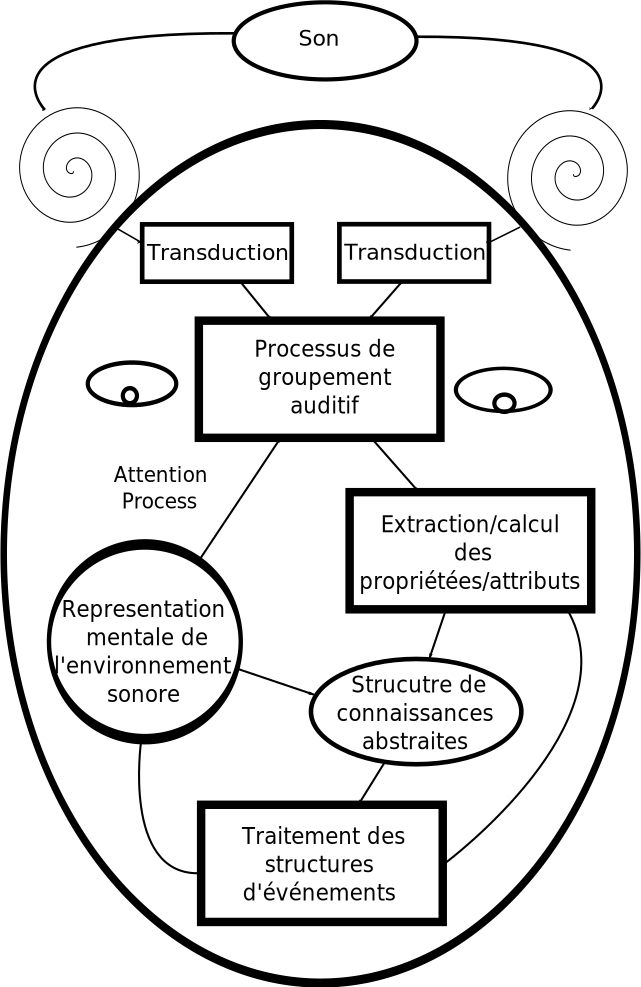
\includegraphics[width=.6\linewidth]{gfx/traitementSonMcAdamsBigand}
        \caption[Principaux processus de traitement de l'information auditive et leurs interactions]{Principaux processus de traitement de l'information auditive et leurs interactions, d'après \citep{mcadams1994penser}}\label{fig:traitementSonMcAdamsBigand}
\end{figure}

Lors de l'étape de \emph{transduction}, les vibrations sonores parvenant au tympan, sont analysées puis traduites en impulsions nerveuses transmises au cerveau. Ces impulsions rendent compte des attributs spectraux et temporels de l'onde. L'extraction des composantes fréquentielles intervient dans la cochlée. C'est à l'intérieur de cette dernière que les différentes parties de la membrane basilaire vont être excitées, en fonction des fréquences composant le signal, suivant un axe tonotopique. Les vibrations, captées à chaque point d’excitation de la membrane basilaire, sont transmises au cerveau via les nerfs auditifs, chaque point codant une information correspondant à une bande fréquentielle limitée. 

Vient ensuite le \emph{processus de groupement auditif}. C'est une étape d'intégration temporelle au cours de laquelle l'information est analysée en images auditives cohérentes. Contrairement à ce que pensaient les Grecs anciens, nous ne possédons pas de "canaux" séparés pour chaque objet sonore présent dans l'environnement \citep{yost1994fundamentals}. C'est notre cerveau qui se charge de fusionner et de discrétiser les éléments sonores simultanés, afin de créer un flux auditif structuré. En d'autres termes, il détermine le nombre d'objets présents, identifie leur provenance, et en définit le sens. 

Afin d'illustrer notre propos, mettons nous dans la peau du mélomane écoutant cette fois un Choral de Bach. C'est le \emph{processus de groupement auditif} qui, sur la base des paramètres spectro-temporels du signal, nous permet de distinguer les voix de basse, ténor, alto et soprano. Les travaux menés au titre de l'Analyse de Scènes Auditives (ASA), dont le sujet est abordé plus bas (\cf~Section~\ref{sec:ch3_ASA}), ont largement porté sur ces processus de groupement.

Ces processus de groupement précèdent généralement la phase dite \emph{d'extraction/calcul des propriétés/attributs}. C'est lors de cette phase que sont extraites les qualités perceptives des objets groupés, ces qualités pouvant être vues comme des propriétés cognitives de haut niveau. pour revenir au choral, c'est à partir d'une analyse des attributs perceptifs que nous sommes capables de percevoir les mélodies comme des objets unitaires, même si celles-ci sont développées entre les différentes voix.

Les phases de groupement et d'extraction concernent l'élaboration et l'analyse d'entités mentales. Une fois représentées dans le cerveau, ces entités sont interprétées pendant l'étape de \emph{structure des connaissances abstraites}. C'est lors de cette étape qu'elles sont identifiées, et qu'un sens interprétatif leur est donné. En pratique, il s'agit de déterminer si le Choral est plaisant ou non.

L'étape suivante, nommée \emph{Traitement des structures d'événements}, permet d'intégrer dans le processus cognitif différents contextes, comme par exemple le contexte fonctionnel (dans quel cadre ce son est-il entendu ?), ou encore le contexte sensoriel (l'information visuelle, ou la mémoire des événements sonores précédemment entendus). Pour revenir à notre mélomane, c'est cette étape qui lui permet d'envisager un morceau dans son ensemble, et, dans le cas d'une fugue, d'entendre que la strette finale est un résumé condensé des sujets précédemment exposés.

La dernière étape du processus de traitement est l'élaboration d'une représentation mentale de l'environnement perçu. C'est au cours de cette étape que nous organisons et conservons les différentes informations extraites. La nature et la formation des représentations mentales sont abordées à la section suivante.

\section{Représentation mentale de l'environnement sonore}
\label{sec:ch3_representationMentale}
 
\gl{TODO: être moins prétentieux, ajouter "il semble, il est utile, il est communément admis"}
 
Le cerveau entretient un dialogue constant avec l'environnement sonore. Ce dialogue s'effectue par le biais des représentations mentales. Une définition des représentations mentales est donnée par \citep{houde1998vocabulaire}:

\begin{quote}
``\,La représentation mentale peut être vue comme une entité interne, le correspondant cognitif individuel des réalités externes expérimentées par un sujet.\,''
\end{quote}

Ces représentations font office de sauvegardes de l'information. Conservées en mémoire sous une forme abstraite \citep[p. 357]{mcadams1994penser}, elles rendent compte à la fois de notre compréhension du monde, et de la manière dont nous l'abordons. Ces connaissances subjectives, non directement observables, restent néanmoins accessibles au chercheur par le biais d'expériences d'objectivation (voir section~\ref{sec:ch3_appCategorielle})
 
Ces représentations forment une image mentale discrète d'un monde réel continu \citep{houde1998vocabulaire}. C'est par le passage du continu au discret que nous sommes à même d'organiser nos connaissances, afin de les réutiliser de manière efficace. Les objets discrets issus de cette organisation sont appelés des catégories. L'action consistant à juger si un événement perçu appartient à une catégorie, est appelée la catégorisation.

\subsection{La notion de catégorie}

\subsubsection{Définition}

Une des vérités de tout être humain est de segmenter son environnement, \ie~de se bâtir un système de classification permettant de regrouper des objets n'étant pas identiques \citep[p. 1]{rosch1978cognition}. On appelle catégorisation, l'action consistant à regrouper des objets du monde physique considérés comme équivalents, et catégorie, l'entité mentale contenant le groupe d'objets ainsi rassemblés. 
 
D'un point de vue écologique, la catégorisation est un processus essentiel. Nous sommes constamment en train de catégoriser l'environnement, et devons être à même, à tout moment, de prendre une décision sur l'appartenance catégorielle d'un objet. Ce processus est adaptatif. La prise de décision est toujours fonction du sujet, d'une situation et d'un contexte. Ainsi, un même objet, perçu à deux moments distincts, pourra être affecté à des catégories différentes. 


\gl{\citep{anderson1991adaptive} propose trois exemples de manifestations quotidiennes des catégories:}

\begin{itemize}

\item le langage: Le langage est le lieu, par excellence, des catégories. Catégoriser, c'est considérer un objet comme un élément distinct du monde. Cette distinction s'accompagne généralement (pas toujours) d'une désignation. C'est l'essence même des processus d'identification que de chercher à nommer les objets, une fois qu'ils ont été isolés. Il est raisonnable de penser que, de la même manière, une catégorie possède un label associé. On parlera alors de catégorie sémantique. Cette relation entre langage et catégorie nourrit le débat sur l'universalité présupposée de la catégorisation. L'opération permanente consistant à isoler un objet, et à lui attribuer un nom, est l'antinomie du ``\,geste adamique\,'', \ie~d'attribution libre du nom, hors toute influence et/ou contexte (d'Adam, le premier homme révélé et nommé dans la bible). La langue est un code partagé par une communauté. Dans une certaine mesure, sa définition, \ie~le sens donné aux mots, peut varier suivant les groupes de cette communauté. Ainsi, catégoriser ne dépend pas seulement d'une réalité physique du monde, mais également d'un contexte socioculturel. La catégorisation peut être vue comme une action intermédiaire entre, d'une part, l'organisation d'une connaissance individuelle résultant d'une expérience sensorielle personnelle, et, d'autre part, la constitution d'une représentation collective pouvant être partagée par le biais d'un langage commun \citep{dubois2006cognitive}.
\item le regroupement par similarité des caractéristiques: Nous sommes capables de regrouper des objets possédant des caractéristiques similaires, et ce, même si ces objets nous sont inconnus \citep{fried1984induction}.
\item le regroupement par similarité fonctionnelle: Nous sommes capables d'interpréter des objets possédant des fonctions similaires comme faisant partie d'un même groupe, et ce même si ces objets ont des caractéristiques distinctes. Pour exemple: deux hommes descendant d'un camion de pompier pour éteindre un feu de forêt seront catégorisés pompiers, ce indépendamment des tenues qu'ils portent. Quand nous parlons de la catégorisation comme du processus de discrétisation du monde réel, ce "monde réel" englobe et la réalité des faits physiques, et la réalité des faits sociologiques.
\end{itemize}

\subsubsection{La nature des catégories}

Toute opération permettant de ``\,voir un objet comme étant $\ldots$\,'' plutôt que de simplement ``\,voir un objet\,'' relève de la catégorisation. Tous les objets peuvent être catégorisés, quelque soit leur nature \citep{goldstone2003concepts}. Reconnaître un animal comme étant un éléphant est un acte catégoriel. Identifier qu'un morceau de musique est le premier mouvement d'une sonate, et qu'il est issu de la période classique, relève également d'un processus de catégorisation. La catégorisation intervient donc sur des objets de différentes natures. On distingue généralement trois types de catégories:

\begin{itemize}
\item catégories naturelles: Regroupe des objets existant à l'état naturel (animaux, fleur, \etc);
\item catégories artificielles: Regroupe des objets fabriqués par l'homme (voiture, outils);
\item catégories de concepts:  Regroupe des objets abstraits qui ne sont ancrés dans une réalité physique (art, stratégie, sentiments).
\end{itemize}

Ces trois types de catégories groupent des objets sur la base de leurs similarités. Pour les catégories d'objets naturels et artificiels, ces similarités s'établissent majoritairement à partir de leurs caractéristiques physiques. Pour les catégories de concepts, ces similarités relèvent d'attributs cognitives plus haut niveau. De plus, qu'ils soient abstraits ou concrets, ces objets ont une existence avérée,\ie~indépendante du contexte.

Cependant, certaines situations particulières poussent à grouper des objets parfaitement dissimilaires, \eg~la liste de courses. Les catégories inhérentes à de tels groupements sont nommées \emph{ad hoc} \citep{barsalou1983ad}:

\begin{itemize}
 \item catégories \emph{ad hoc}:  regroupent des objets afin de répondre à un besoin spécifique.
\end{itemize}

\subsection{Le processus de catégorisation}

\subsubsection{Catégorisation et prédiction}
\label{sec:ch3_categoPred}

La structure catégorielle forme la base des ressources cognitives sur lesquels nous nous appuyons afin d'isoler des objets du monde. Ce processus procède de deux mécanismes:

\begin{itemize} 
\item mécanisme inductif: associer un objet à une catégorie sur la base des propriétés perçues de ce dernier;
\item mécanisme déductif: associer à un objet les propriétés de la catégorie à laquelle il appartient.
\end{itemize}

Le mécanisme déductif est d'une importance capitale. Il nous permet de généraliser nos connaissances, \ie~d'inférer les propriétés d'un objet sans pour autant les avoir perçues. Ces propriétés transmises peuvent être physiques ou conceptuelles. Exemple: il suffit de voir la croupe d'un cheval pour en "déduire" l'animal. Autre exemple: le bourdonnement d'un insecte peut laisser supposer la présence d'une guêpe, et susciter le sentiment du danger. On le voit, le mécanisme déductif nous permet d'aller au delà de l'information perçue, mais peut également mener à des erreurs d'interprétation. Notre capacité d’adaptation est très liée à ce mécanisme.

\subsubsection{Catégorie et langage}
\label{sec:ch3_catLang}

\gl{TODO}

\subsubsection{Catégorisation et identification}

On distingue généralement les processus de catégorisation, et les processus d'identification.  La catégorisation, \ie~regrouper des objets en classes d'équivalences, est un processus pouvant s'opérer dans un cadre non-supervisé, \ie~sans avoir besoin de nommer les classes. L'identification, quant à elle, est nécessairement supervisée, \ie~nous ne pouvons identifier des objets qu'à partir des catégories que nous connaissons. Ainsi, si un très jeune enfant voit pour la première fois un groupe de hyènes dans un zoo, il interprétera ces animaux comme faisant partie de la même espèce. Cependant, il a de très grandes chances d’identifier l'espèce comme ``\,une sorte de chien\,''.


Ces deux processus sont pourtant très liés \citep{goldstone2003concepts}, l'identification pouvant être vue comme un cas particulier de la catégorisation \citep{schyns1998diagnostic}. Nos travaux ne requérant pas de distinguer ces deux mécanismes, nous considérons, dans ce document, la catégorisation au sens large, incluant l'identification.

\subsection{Organisation de la structure catégorielle}

Le cerveau doit en permanence faire sens d'une information riche et variée, et ce de manière productive. Afin de satisfaire à cette exigence d'efficacité, l'organisation  de la structure catégorielle doit répondre à deux grands principes \citep[p. 29]{rosch1978cognition}:

\begin{itemize}
\item l'économie cognitive;
\item la redondance structurelle.
\end{itemize}

\subsubsection{L'économie cognitive}

La catégorisation doit fournir un maximum d'informations pour un minimum d'efforts. C'est pourquoi la logique catégorielle prend en compte le contexte sensoriel. En résumé, le traitement de l'objet s'opère et par rapport à lui, et par rapport au traitement des objets perçus et catégorisés simultanément. Comme énoncé par D. Dubois \citep[p. 33]{dubois1991semantique}:

\begin{quote}
``\,Catégoriser un stimulus signifie le considérer dans la finalité de cette catégorisation, non seulement comme équivalent des autres stimuli de la même catégorie, mais également différent des stimuli qui n'appartiennent pas à cette catégorie\,''.
\end{quote}

Du principe d'économie cognitive, il découle que la catégorisation de l'objet n'est pas une catégorisation dans l'absolu. Elle ne dépend pas uniquement de l'observation des propriétés particulières de l'objet, mais également du contexte dans lequel il est appréhendé.

\subsubsection{La redondance structurelle}

L'ensemble des objets physiques ne vit pas dans un espace fini, identifié, et dont les valeurs seraient équiprobables. Le monde ne se résout pas à des paramètres dimensionnés, indépendants et manipulables, comme dans le cadre d'études en laboratoire. Au contraire, il peut exister des discontinuités saillantes entre objets, de même que ces objets peuvent être liés entre eux par des patterns de co-occurrence de propriétés (exemple : un chien possède "quatre pattes et un museau" plus souvent que "deux pattes et un museau"). Ces discontinuités et corrélations, présentes dans les propriétés perçues, étayent la structure catégorielle de notre représentation mentale, et gouvernent ainsi le processus de catégorisation.
 
\subsubsection{Catégorie et abstraction}
 \label{sec:ch3_categoEtAbstract}
 
Pour des catégories d'objets concrets (naturels ou artificiels), Rosch propose de voir la structure catégorielle suivant deux axes \citep[p. 30-41]{rosch1978cognition}:

\begin{itemize}
\item \textit{axe vertical}: L'axe vertical fixe l'organisation hiérarchique des catégories, et permet d'appréhender l'imbrication de ces catégories les unes par rapport aux autres. Ce faisant, il en dresse la taxonomie, les catégories de haut niveau représentant des objets abstraits ou concepts, et incluant un grand nombre de sous catégories, et les catégories de bas niveau représentant des objets concrets, incluant peu de sous catégories. Ainsi, plus le niveau d'abstraction est grand, plus les similitudes entre objets d'une même catégorie (intra-catégorielle), ainsi que les similitudes entre objets de catégories distinctes (inter-catégorielle) sont faibles. Inversement, plus le niveau d'abstraction est faible, plus les similitudes intra- et inter-catégorielles sont élevées. Rosch décompose cette dimension verticale en trois niveaux d'abstraction (\cf~Figure~\ref{fig:categorieLVL}): superordonné, base et subordonné. Le niveau superordonné regroupe les catégories à haut niveau d'abstraction. Les périmètres de ces catégories sont larges (Mobilier, Véhicule...) \ie~les objets qu'elles contiennent peuvent être très distincts. Le niveau subordonné regroupe les catégories à bas niveau d'abstraction, ou catégories concrètes. Les périmètres de ces catégories sont plus précis (Chaise longue, Cabriolet...), et les objets qu'elles contiennent sont nécessairement très similaires. On notera ici que les objets de la classe Cabriolet présentent plus de propriétés communes avec les objets de la classe Berline, que n'en sauraient partager les objets des classes Mobilier et Véhicule. Au niveau de base, les objets d'une même catégorie partagent encore beaucoup de propriétés en commun, tout en maintenant une dissimilarité inter-catégorielle élevée.
\item \textit{axe horizontal}: L'axe horizontal fixe, lui, l'organisation ``\,géographique\,'' des catégories, et permet d'appréhender, d'une part, les périmètres de ces catégories au sein d'un même niveau d'abstraction, d'autre part, la typicalité des objets contenus dans une même classe. Les catégories ne sont pas des objets strictement discrets, et les propriétés des objets qu'elles regroupent peuvent se trouver attribuées à d'autres objets, dans d'autres catégories. Ainsi, les frontières entre les différentes catégories ne sont pas figées, et peuvent même se recouvrir.
\end{itemize}

\gl{On remarque que l'organisation de nos connaissances, ainsi représentées par la structure catégorielle, forme un miroir de la redondance structurelle inhérente au monde physique. Selon \citep[p. 28]{rosch1978cognition}, c'est le niveau de base qui rend compte au mieux de cette structure. Il s'agit d'un niveau privilégié, proposant le meilleur compromis entre le nombre de catégories et l'information qu'elles véhiculent. Il permet ainsi d'obtenir le maximum d'informations au prix d'un moindre effort cognitif.}

Cependant, si cette vision bidimensionnelle de la structure catégorielle est adaptée aux catégories d'objets concrets, elle est moins pertinente dans le cas des catégories de concepts, comme les catégories sociales \citep[p. 72-88]{dubois1991semantique}. Considérer l'organisation catégorielle comme le reflet du monde perçu vaut surtout en ce qui concerne le monde physique.

\begin{figure}[t]
        \myfloatalign
        \includegraphics[width=.6\linewidth]{gfx/categorieLVL}
        \caption{Les trois niveaux d'abstraction de l'axe vertical de la structure catégorielle.}\label{fig:categorieLVL}
\end{figure}

\subsubsection{La notion de typicalité}
\label{sec:ch3_typicité}

Une notion clef, dans les processus catégoriels, est la typicalité. Tous les objets d'une catégorie ne sont pas égaux. Il y a une gradation dans l'appartenance catégorielle. Certains objets, partageant les propriétés dominantes d'une catégorie, sont considérés comme très représentatifs de cette dernière, d'autre encore, ne partageant que peu des attributs caractéristiques de la catégorie, ont une appartenance moins marquée.

Le fait qu'il existe des objets plus typiques que d'autres est un constat empirique \citep[p. 37]{rosch1978cognition,mervis1981categorization}, établi à partir d'échelles de jugements (quel est l'objet le plus typique ?) ou au moyen d'épreuves de vérifications chronométrées (un chien est il un animal: vrai ou faux ?) \citep[p. 41]{dubois1991semantique}.

La typicalité agit sur différents processus de traitement \citep[p. 51]{Houix03f,mervis1981categorization}:

\begin{itemize}
\item \emph{temps de traitement}: un objet typique est catégorisé plus rapidement qu'un objet moins typique;
\item \emph{apprentissage}: un enfant bâtit sa structure catégorielle en commençant d'abord par des objets typiques;
\item \emph{ordre mémoriel}: lorsqu'un sujet énumère les membres d'une catégorie, il commence par les membres typiques;
\item \emph{langage}: certains termes du langage courant sont directement connectés à la typicalité, ainsi, un ``\,moineau est un \emph{vrai} oiseau\,'', alors qu'un ``\,pingouin est une \emph{sorte} d'oiseau\,'' \citep{mervis1981categorization};
\item \emph{asymétrie des jugements de ressemblance}: il existe un phénomène d'attraction autour des objets typiques d'une catégorie: si nous considérons la catégorie couleur, l’orange ressemble plus au rouge que le rouge ne ressemble à l'orange. L'asymétrie dans les processus perceptifs a été extensivement étudiée \citep{tversky1977features,krumhansl1978concerning}.\gl{TODO: préciser en quoi l'attraction implique l’asymétrie}
\end{itemize}


\subsection{Théories de la catégorisation}

\subsubsection{Théorie classique}

Suivant les principes de l'approche logique, dite aussi approche par règles, l'appartenance d'un objet à une catégorie se fait sur la base de règles. L'objet doit posséder un certain nombre de propriétés afin d'être assimilé à une catégorie. La nature de ces propriétés étant inhérentes à la catégorie.

Cette approche, qui sous-tend que tous les objets d'une catégorie doivent partager des propriétés communes, est aujourd'hui critiquée. Selon \citep{goldstone2003concepts}:

\begin{itemize}
\item l'appartenance catégorielle n'est pas figée: deux personnes peuvent catégoriser un même objet de deux manières. Qui plus est, une même personne peut modifier sa stratégie de catégorisation \citep{mccloskey1978natural};
\item les objets ne partagent pas le même degré d'appartenance: comme vu précédemment (\cf~Section~\ref{sec:ch3_typicité}, tous les objets à l'intérieur d'une catégorie ne sont pas égaux, certains étant plus typiques que d'autres.
\item il est difficile de définir des règles d'appartenance: définir des catégories comme ``\,célibataire\,'' nécessite d'élaborer des stratégies afin d'isoler les cas ``\,enfants\,'', ``\,veuf\,'' ou encore ``\,pape\,'' qui, intuitivement, n'ont rien à voir avec ``\,célibataire\,'' \gl{TODO: peu clair ?}. 
\end{itemize}

De plus, \citep[49]{Houix03f} souligne que, dans l'approche logique, les classes subordonnées héritent des règles d'appartenance des classes superordonnées, niant ainsi le fait qu'il existe des niveaux d'abstractions privilégiés. 

\subsubsection{Théorie prototypique}

Une alternative à l'approche classique, consiste à envisager la catégorie non plus comme relevant de règles, mais comme découlant, en quelque sorte, de la ressemblance ou ``\,air de famille\,'' liant ses membres \citep{ludwig1953philosophical}.

Partant de cette idée, la théorie prototypique a été formalisée par E. Rosch et B. B. Lloyd \citep{rosch1978cognition}. Dans celle-ci, la catégorie est définie par rapport aux objets qu'elle englobe, et non dans le but d'englober ces objets.

Pour discriminer les catégories, Rosch propose de ne pas raisonner en terme de frontières, mais plutôt de décrire chaque catégorie par un nombre de cas non ambigus (\emph{clear case}) \citep[p. 36]{rosch1978cognition}. Tous les objets d'une catégorie ne sont pas également représentatifs de cette dernière. Il a été montré que des sujets peuvent très bien s'accorder sur la typicalité d'un objet par rapport à une catégorie, tout en n'étant pas d'accord sur les frontières de cette dernière \citep{rosch1974human,rosch1975cognitive}. Les cas non ambigus peuvent être vus comme les objets les plus typiques de la catégorie. Le terme prototype, qui donne son nom à la théorie, vient de l'assertion que, parmi ces cas non ambigus, il en existe un, le prototype, plus représentatif que les autres, et qui forme le noyau de la catégorie.

Les catégories sont structurées en interne, en référence à un prototype, \ie~l'objet possédant les attributs typiques de celle-ci. L'appartenance d'un objet à une catégorie dépend alors de la ressemblance qu'entretient ce dernier avec le prototype.  Plusieurs propositions ont été faites afin de définir le prototype d'une catégorie: Pour Tversky \citep{tversky1977features}, l'élément prototype est celui dont la somme des similarités avec les autres éléments de la catégorie est la plus élevée. Pour \citep{rosch1975family}, il s'agit de l'objet possédant le plus de propriétés en commun avec les objets de la catégorie, et le moins de propriétés avec les objets des catégories externes. La typicalité d'un élément d'une catégorie s'évalue à la fois en fonction de son degré d'appartenance à celle-ci, et de son degré de différenciation vis à vis des autres catégories. 

Toutes ces approches supposent que le prototype est la représentation mentale d'un objet réel. Cependant, le prototype peut être aussi être vu comme un objet stéréotypé, un assemblage des attributs les plus représentatifs de la catégorie. Ainsi, en se limitant à l'observation d'attributs vivant dans un espace métrique, \citep{reed1972pattern, rosch1976structural} ont montré que le prototype est un centroïde, un objet défini comme étant la moyenne des attributs des objets de la catégories. \gl{TODO: Préciser qu'on retrouve cette différence entre le centroïde et le medoïde}

Cette théorie prototypique de la catégorisation, bien que se basant sur des faits expérimentaux, est avant tout une vision pratique, un concept qui n'a pas été clairement défini et dont l'implication dans les processus de catégorisation reste floue \citep[p. 36-40]{rosch1978cognition} \citep[p. 49-54]{dubois1991semantique}.

\subsubsection{Théorie des exemplaires}

La théorie des exemplaires nie l'existence d'un prototype. Au contraire, elle propose que la catégorie soit représentée sur la base de tous les objets (exemplaires) la constituant, en tenant compte de leurs degrés de typicalité respectifs \citep{medin1978context,nosofsky1986attention,nosofsky1992similarity}. Ainsi, les mécanismes déductifs (\cf~Section~\ref{sec:ch3_categoPred}) peuvent profiter de tout les exemplaires de la catégorie afin d'inférer les propriétés des objets perçus. En analyse automatique, la philosophie de l'approche par les exemplaires est proche de celle des cartes auto-organisées (\emph{Self organized map}) \citep{kohonen1995som}, l’organisation du réseau et de ses nœuds étant réactualisée en fonction des propriétés de tous les items.

Plusieurs versions de cette théorie existent, entre autres, le modèle de contexte \citep{medin1978context}, et le modèle de contexte généralisé \citep{nosofsky1986attention}. Dans le modèle de contexte, les objets sont représentés suivant leurs attributs, la dimension de l'espace de représentation étant alors égale aux nombres d'attributs, choisis dans un contexte particulier \citep{hitzman1986schema}. Dans le modèle généralisé, les objets sont représentés dans un espace psychologique aux dimensions réduites, espace établi sur la base des distances inter-objets \citep{nosofsky1992similarity}. Typiquement, le positionnement dimensionnel (\cf~annexe~\ref{app:mds}) est utilisé afin de recouvrir de tels espaces.

Dans la théorie des exemplaires, l'appartenance catégorielle se fait sur la base de la somme pondérée des similarités entre l'objet à catégoriser, et les exemplaires de la catégorie. Dans le modèle de contexte, la pondération s'effectue sur les propriétés des objets, et rend compte d'un poids attentionnel, favorisant les propriétés saillantes dans un contexte donné. Dans le modèle généralisé, la pondération se fait en fonction de la distance entre les exemplaires et l’objet, et ce afin de favoriser les exemplaires proches de l'objet à catégoriser.

L'approche par les exemplaires lève cependant deux questions \citep{goldstone2003concepts}:

\begin{itemize}
\item Comment justifier que nombres d'études montrent que l'appartenance catégorielle s'effectue via une comparaison à un prototype ?
\item Comment justifier que le principe d'économie cognitive reste valide, si le cerveau utilise l'ensemble des items d'une catégorie pour la représenter ? 
\end{itemize}

Dans la théorie des exemplaires, la proximité entre un objet et une catégorie est la somme des similarités entretenues entre l'objet et les items de la catégorie \citep{nosofsky1986attention}. Dans certains cas, cette opération équivaut à calculer la similarité entre l'objet et le représentant moyen des items de la catégorie. L’existence d'un prototype n'est alors qu'un artefact. Notons quand même que la théorie des exemplaires ne nie pas l'existence d'un gradient de typicalité entre les objets d'une catégories.

Bien qu'on puisse montrer, dans le cas d'un bruit blanc, que le cerveau peut stocker en mémoire la totalité d'un signal sur une période de plusieurs semaines  \citep{agus2010rapid}, il est écologiquement peut probable que, pour chaque catégorie, le cerveau sauvegarde la totalité des exemplaires. Deux phénomènes peuvent alors intervenir: soit il existe un processus de sélection des exemplaires \citep{palmeri1995recognition}, soit les exemplaires émanant d'une même entité physique (deux exemples de pigeon), sont résumés par un même représentant \citep{barsalou1998basing} \gl{TODO: a nuancer, ces deux options sont triviales et les processus de mémorisation sont plus complexes}.

\subsubsection{Théorie des frontières}

En opposition directe avec le modèle prototypique, la théorie des frontières représente les catégories par leur périphérie. L'importance des frontières est un fait expérimental mis en avant par plusieurs études. Notamment \citep{davis2010memory} qui montre que, dans le cas de deux catégories proches, l'objet représentatif putatif n'est pas le prototype, mais une caricature de ce dernier. La caricature du prototype est une entité dont les propriétés ont été distordues afin qu'elle s'éloigne de la frontière séparant les deux catégories, distorsion qui peut substantiellement éloigner la caricature des objets de sa catégorie (\cf~Section~\ref{fig:prototypeCaricature}).

\citep{goldstone2003concepts} souligne que les théories du prototype et des frontières peuvent se compléter: pour des catégories très éloignées, la distance au prototype (représentant moyen des objets d'une catégorie) est une information suffisante pour associer l'objet à une catégorie. Pour des catégories très similaires, l’appartenance catégorielle, afin d'être efficace, doit s'appuyer sur une information plus spécifique, à savoir la frontière.

Par ailleurs, la théorie des frontières n'envisage pas la périphérie d'une catégorie comme quelque chose de statique. Il existe une frontière a priori, certes, mais cette dernière peut bouger en fonction du contexte.

\begin{figure}[t]
        \myfloatalign
        \includegraphics[width=.8\linewidth]{gfx/prototypeCaricature}
        \caption[Prototype et caricature]{Prototype et caricature, d'après \citep{davis2010memory}}\label{fig:prototypeCaricature}
\end{figure}

\subsection{Similarité et catégorisation}

G0: \citep{gygi2007similarity}

\subsection{Catégorisation et contexte sensoriel}
\label{sec:ch3_identification et Contexte}

G1: \citep{ballas1987interpreting,niessen2008disambiguating,gygi2011incongruency} \\


\section{Analyse de scènes acoustiques}
\label{sec:ch3_ASA}

\gl{TODO: plus insister sur la notion de flux, lien chapitre 4}

\subsection{Définition}
\label{sec:ASAintro}

L'analyse de scène est un procédé issu de la recherche dans le domaine de la vision, où les études portent notamment sur les stratégies suivies par l'ordinateur pour parvenir à isoler un(des) objet(s), ou une structure, d'une image~\citep[p. 12]{mcadams1994penser}. Dans le domaine de l'audition, un procédé analogue est appelé Analyse de Scène Acoustique. L'ASA a été introduite par A. S. Bregman dans son ouvrage de référence \citep{bregman1994auditory}.

L'ASA désigne l'ensemble des traitements perceptifs permettant d'isoler, dans une mixture sonore, les informations émanant de sources distinctes, et de les ``\,organiser\,'' en un tout cohérent. Ces regroupements sont nécessaires au cerveau, et donc au sujet, pour comprendre, pour donner sens à l'environnement. On parle de processus de ségrégation ou de processus de groupement \citep{winkler2009modeling}. Comme vu précédemment à la section~\ref{sec:chaineTaite}, ces processus mobilisent à la fois les traitements ascendants ou \emph{bottom-up}, intervenant au niveau de l'information auditive transduite, et les traitements descendants ou \emph{top-down}, intervenant au niveau du bagage mémoriel. Les processus \emph{bottom-up} sont appelés ``\,processus primitifs\,'', et les processus  \emph{top-down}, ``\,processus basés sur des schémas\,''. 

Les processus primitifs sont innés, et opèrent à partir des régularités du signal, afin d'en regrouper les composantes fréquentielles produites par une même source. Le mot régularité désigne ici les propriétés constantes de l'environnement, perçues par tous les individus, et en tous lieux. Par exemple, si la fréquence fondamentale d'un son harmonique change au cours du temps, toutes ses harmoniques changeront également afin de maintenir la structure harmonique du son [p. 38]\citep{bregman1994auditory}.

Les processus basés sur des schémas sont, eux, conditionnés, et opèrent sur la base de connaissances, ou schémas, partie intégrante de notre représentation mentale du monde, représentation construite à partir des écoutes antérieures. 
 
\subsection{Une approche psychoacoustique}

Si la plupart des recherches sur l'ASA adoptent une approche cognitiviste, se concentrant sur l'étude des \emph{processus primitifs}, elles suivent généralement une méthodologie expérimentale très inspirée de la psychoacoustique. De fait, les sujets sont soumis à des stimuli décrits analytiquement dans un espace multidimensionnel de dimensions physiques (fréquence, intensité, \etc) \citep{dubois2006cognitive}. Dans la majorité des cas, ces stimuli, ou sons, qu'ils soient purs ou qu'ils soient complexes,\footnote{Un son pur est un son composé d'une seule sinusoïde, \ie~possédant une seule fréquence. Un son complexe est, lui, composé de plusieurs composantes fréquentielles} sont synthétisés en laboratoire.

Ces sons sont émis de manière séquentielle. Au cours de l'expérience, les paramètres d'écoute sont modifiés (intensité, hauteur fréquentielle, espace entre les séquences...) afin d'évaluer le seuil à partir duquel la capacité du sujet à distinguer les sources sonores est altérée.

L'ASA \gl{se focalise donc sur} l'analyse de l'effet de descripteurs ``\,bas niveau\,'' dans le processus d'intégration, sans tenir compte d'attributs perceptifs ``\,haut niveau\,'', comme la valeur sémantique attribuée aux sons, sans tenir compte non plus de considérations écologiques (\cf~Section~\ref{sec:ch3_ecologique}). Il est difficile de faire un parallèle entre la notion de source sonore utilisée dans le domaine de la psychoacoustique, et celle admise dans le domaine de la psychologie cognitive. Dans l'une et l'autre approche, a priori, le terme source sonore s'applique à l'objet source (\eg~voiture). C'est évident en psychologie cognitive, où le stimulus est le plus souvent un enregistrement de ladite source. Cela l'est moins en psychoacoustique, où le stimulus, synthétisé, est un objet abstrait (agglomérat de sinusoïdes), éloigné de la réalité des phénomènes acoustiques, et dont l'existence n'est avérée que dans la mesure où il est interprété par le sujet comme un tout, une entité. Les résultats obtenus à partir de ces stimuli sont difficiles à généraliser à des applications plus incarnées.

\subsection{Régularités et processus primitifs}

\begin{figure}[t]
        \myfloatalign
        \subfloat[]
        {\includegraphics[width=.5\linewidth]{gfx/tonesim_slow-eps-converted-to}}
        \subfloat[]
        {\includegraphics[width=.5\linewidth]{gfx/tonesim_fast-eps-converted-to}}
        \caption[Groupement séquentiel : proximité temporelle.]{Groupement séquentiel: proximité temporelle. Dans l'exemple (a), la durée entre les événements est importante, aucun groupement n'est effectué, les sons sont perçus comme des événements distincts. Dans l'exmple (b) la durée entre les événements est réduite, un groupement s'opère suivant la proximité fréquentielle. Deux flux sont ainsi créés, le premier (rouge) regroupe les sons haute fréquence, le deuxième (vert), les sons basse fréquence.}\label{fig:tonesim}
\end{figure}

\begin{figure}[t]
        \myfloatalign
        \subfloat[]
        {\includegraphics[width=.5\linewidth]{gfx/gallop_2flux-eps-converted-to}}
        \subfloat[]
        {\includegraphics[width=.5\linewidth]{gfx/gallop_1flux-eps-converted-to}}
        \caption[Groupement séquentiel : proximité fréquentielle.]{Groupement séquentiel: proximité fréquentielle. Deux groupes de sons sont joués à deux fréquences. Dans l'exemple (a), la distance entre les fréquences des sons est importante, deux flux sont créés, le premier (rouge) regroupe les sons haute fréquence, et le deuxième (vert), les sons basse fréquence. Dans l'exemple (b) la distance entre les fréquences est réduite, un groupement s'opère suivant la proximité fréquentielle. Un seul flux est créé, et l'on perçoit un motif temporel, ici, le galop d'un cheval.}\label{fig:galop}
\end{figure}

L'existence des \emph{processus primitifs} est une conséquence de l'efficience, dans le monde sonore, de régularités universelles affectant l'ensemble des stimuli auditifs. Bregman distingue 4 types de régularités [p. 19,21,31,33]\citep{mcadams1994penser}:

\begin{enumerate}
\item \emph{synchronicité}: il est rare que des sons n'ayant aucun rapport entre eux démarrent et s'arrêtent au même moment;
\item \emph{continuité}: 
\begin{itemize}
\item les propriétés d'un son isolé tendent à se modifier lentement et de façon continue;
\item les propriétés d'une séquence de sons émis par la même source tendent à se modifier lentement.
\end{itemize}
\item \emph{harmonicité}: lorsqu'un corps sonore vibre à une période répétée, ses vibrations donnent naissance à un motif acoustique dont les fréquences des composants sont des multiples d'une même fréquence fondamentale;
\item \emph{uniformité}: la plupart des modifications qui surviennent dans un signal acoustique affectent tous les composants du son résultant, de manière identique, et simultanée.
\end{enumerate}

Notre perception du monde est assujettie à ces régularités. 
Les \emph{processus primitifs}, sensibles aux stimuli exclusivement, nous permettent d'isoler du monde sonore des objets cohérents, perçus à travers elles \citep{ballas1987interpreting}. Le fait est qu'un principe similaire de perception des formes s'applique également au domaine de la vision.

\subsection{Perception de la forme}

\begin{figure}[t]
        \myfloatalign
        \includegraphics[width=.5\linewidth]{gfx/harmo-eps-converted-to}
        \caption[Groupement simultané : régularité harmonique]{Groupement simultané : régularité harmonique. Un son complexe est joué plusieurs fois. A chaque occurence, on abaisse les hauteurs de la fréquence fondamentale et des harmoniques, de manière uniforme. Un harmoniqu est conservé à fréquence constante (trait gras). Au début, un flux est créé, \ie~les harmoniques et la fréquence fondamentale sont perçus comme étant un seul objet. Au fur et à mesure que la régularité harmonique est brisée, le cerveau tend à percevoir l'harmonique à fréquence constante dans un flux séparé, \ie~comme étant un second objet.}\label{fig:harmo}
\end{figure}

\begin{figure}[t]
        \myfloatalign
        \subfloat[]
        {\includegraphics[width=.5\linewidth]{gfx/opn1-eps-converted-to}}
        \subfloat[]
        {\includegraphics[width=.5\linewidth]{gfx/opn2-eps-converted-to}}
        \caption[Groupement ancien-plus-nouveau]{Groupement ancien-plus-nouveau. Dans l'exemple (a), les sons A et B ont des fréquences éloignées. Le cerveau génère deux flux, le premier relatif au son A (rouge), et le deuxième comprenant les sons B et C (vert). Dans l'exemple (b), les sons A et B ont la même fréquence. Le cerveau interprète le son B comme étant une continuité du son A. L'attraction entre B et C en est réduite. Le cerveau génère toujours deux flux, le premier regoupant cette fois les sons A et B (rouge), et le deuxième le son C (vert).}\label{fig:oldplusnew}
\end{figure}

Que ce soit en vision ou en audition, notre cerveau est en permanence stimulé par une multitude de sources distinctes. Percevoir un objet dans cet agglomérat, c'est être capable d'isoler tous les signaux émis par une même source, et de les réunir en une unité perceptive cohérente.

Parmi les premiers travaux qui se sont intéressés à ces processus de groupement, on trouve la psychologie de la forme, en allemand \emph{Gestalttheorie}. Cette théorie, introduite par Ernst Mach et Christian von Ehrenfels à la fin du XIXème siècle, explicite les principes selon lesquels des stimuli sensoriels sont combinés, afin de former un pattern mental rendant compte de la présence d'un objet dans un environnement donné.

Mis en évidence en perception visuelle, ces principes restent vrais en perception auditive \citep[ch. 1]{bregman1994auditory}. Parmi ces principes, nous en détaillons ici cinq:

\begin{enumerate}
\item \emph{proximité}: des éléments proches les uns des autres ont tendance à être groupés ensemble. En audition, ce principe de proximité opère suivant les différentes caractéristiques du son, à savoir, la fréquence, l'\emph{onset} \footnote{En traitement du signal audio, on désigne par le mot anglais \emph{onset} le début du signal. Ce terme étant couramment utilisé en français, nous ne le traduirons pas dans ce document.} et l'intensité.
 
\item \emph{similarité}: des éléments qui se ressemblent ont tendance à être groupés ensemble. 

Commentaire. Dans le domaine de la vision, la proximité est une notion de spatialité. La similarité, elle, s'applique aux caractéristiques physiques de l'objet (forme, couleur, etc $\ldots$), qui ne peuvent se décrire dans une dimension unique. 

Dans le domaine de l'audition, la proximité est généralement admise comme notion de temporalité (\emph{onsets} proches). Pour le reste des descripteurs, il est cependant difficile de distinguer les principes de proximité et de similarité. Bregman propose de parler de proximité lorsqu'on traite d'une dimension physique particulière, et de parler de similarité dès lors qu'on considère un ensemble de descripteurs, ou lorsque l'on traite d'attributs qui ne peuvent être clairement décomposés suivant des dimensions distinctes. Exemple: le timbre.

\item \emph{continuité}: des éléments qui varient de manière non abrupte ont tendance à être groupés ensemble. Par ce principe, des objets distincts mais proches temporellement (en vision, proches spatialement) ont tendance à être reçus comme le prolongement des uns par les autres. C'est ce principe qui nous permet de percevoir comme une seule entité un objet dont les caractéristiques varient dans le temps, \eg~le son d'une sirène. \emph{A contrario}, un changement abrupt indique généralement l'apparition d'une nouvelle source.

De récentes études en neurosciences ont montré l'importance de ce principe dans les processus de groupement. \citep{winkler2009modeling}  propose de voir l'ASA comme un processus prédictif, le cerveau cherchant à anticiper la nature des stimuli qui lui parviennent, sur la base de régularités extraites des objets détectés dans l'instant précédant.

\item \emph{clôture}: des éléments discontinus, qui suggèrent la forme d'un objet continu, ont tendance à être groupés ensemble. De manière automatique, le cerveau tend à percevoir un ensemble d'objets distincts comme un tout. En audition, ce principe est très lié à la notion de masquage. En effet, les sons que nous percevons sont régulièrement masqués par d'autres sons concurrents, éventuellement plus forts. Le principe de clôture nous permet de compenser ce phénomène de masquage, et de percevoir le signal sans discontinuité. Ainsi lorsqu'un son pur est régulièrement entrecoupé de silences, nous percevons une série de sons purs, mais, si ces silences sont comblés par un bruit blanc, nous percevons un son pur continu. Ce phénomène est parfois appelé ``\,l’illusion de continuité\,'' \citep{dannenbring1976perceived}, et s'applique particulièrement dans le contexte de la perception de la parole \citep{carlyon2002continuity}.

\item \emph{destin commun}: des éléments qui varient de manière synchrone et uniforme ont tendance à être groupés ensemble. Comme évoqué à la section~\ref{sec:ASAintro} c'est ce principe qui permet de percevoir comme un tout les différents harmoniques qui composent un son complexe. C'est également ce principe qui nous incite à percevoir de manière unie des stimuli ayant le même \emph{onset} temporel.
\end{enumerate}

Ces principes agissent de concert afin de grouper les composantes du son en flux auditifs.

\subsection{Flux auditif et stratégie de groupement}

\begin{figure}[t]
        \myfloatalign
        \subfloat[]
        {\includegraphics[width=.5\linewidth]{gfx/seqsim1-eps-converted-to}}
        \subfloat[]
        {\includegraphics[width=.5\linewidth]{gfx/seqsim2-eps-converted-to}}
        \caption[Compétition entre groupement séquentiel et groupement simultané]{Compétition entre groupement séquentiel et groupement simultané. Dans l'exemple (a), le cerveau perçoit deux flux, le premier regroupant le son A (rouge) et le deuxième regroupant les sons B et C (vert). Dans l'exemple (b), un quatrième son (D) est ajouté, ce dernier possédant une fréquence très proche de celle de (D). Le groupement sequentiel par proximité fréquentielle entre les couples A-B et C-D est favorisé, au détriment du groupement simultané entre les sons B-C.}\label{fig:simvsseq}
\end{figure}

L'une des notions les plus importantes en ASA est le concept de flux auditif (\emph{auditory stream}), que Bregman définit comme ``\,le groupement perceptif que nous faisons des parties du spectre qui vont ensemble\,''.

Contrairement au terme ``\,son\,'', qui peut faire référence aux réalités physiques des phénomènes acoustiques, aussi bien qu'aux représentations mentales que nous nous en faisons, le flux auditif désigne spécifiquement une entité perceptive.

Le terme flux se veut volontairement généraliste. Ce dernier peut désigner aussi bien un son isolé (un coup de marteau), que plusieurs sons, à condition que ces derniers soient perçus comme formant une seule entité (une série de coups de marteau rapprochés).

On désigne par ``\,formation de flux auditifs\,'' (\emph{auditory streaming}) , le processus à l'origine de la création de flux. \citep{winkler2009modeling} proposent la définition suivante en ce qui concerne la formation de flux auditifs:

\begin{quote}
``\, Un phénomène perceptif dans lequel une séquence de sons est perçue comme étant composée de deux ou plusieurs flux auditifs \,''
\end{quote}

Comme nous le voyons, le flux désigne une représentation perceptive d'un son, et, à ce titre, il est l'équivalent auditif de l'objet pour la vision \citep[p. 11]{bregman1994auditory}. Cependant, nous notons que la notion de flux, et plus particulièrement celle de formation de flux, est souvent utilisée dans un contexte où une dimension temporelle est sollicitée. On parle d'ailleurs de construction de flux (\emph{build-up of streaming}) pour désigner la période durant laquelle le cerveau accumule des indices afin de générer et stabiliser les flux auditifs  \citep{cusack2004effects,snyder2007toward}. Ainsi, dans ce document, nous réservons les termes ``\,flux\,'' pour désigner les représentations mentales des stimuli en train d'être traités (intégrés temporellement), et ``\,formation de flux auditifs\,'' pour désigner les processus perceptifs de groupement des sons. Nous conservons le mot ``\,objet\,'' pour désigner, de manière générale, les représentations mentales stockées en mémoire des phénomènes acoustiques.

En ce qui concerne les processus primitifs, on distingue trois stratégies de groupement:

\begin{itemize}
\item \emph{groupement séquentiel}: désigne le groupement de sons ne partageant pas un même \emph{onset}. Dans le cas de sons purs, le groupement séquentiel s'appuie beaucoup sur le principe de \emph{proximité}, et notamment de \emph{proximité} fréquentielle, principe qui veut que, plus deux sons sont proches en fréquence, plus ils ont tendance à être regroupés dans le même flux (\cf~Figure~\ref{fig:galop}). Pour des sons complexes, c'est plutôt le principe de similarité qui entre en jeux. La \emph{proximité} temporelle, \ie~la durée séparant chaque son, rentre cependant en ligne de compte. Plus cette dernière est faible, plus deux sons ont des chances d'êtres regroupés (\cf~Figure~\ref{fig:tonesim});
\item \emph{groupement simultané}: aussi appelé groupement spectral, désigne le groupement des composantes fréquentielles qui partagent un même \emph{onset}. Le groupement simultané s'appuie principalement sur la régularité harmonique. Une composante fréquentielle venant briser la suite harmonique tend à être isolée dans un autre flux auditif (\cf~Figure~\ref{fig:harmo});
\item \emph{groupement ancien-plus-nouveau}: Ce groupement est l'application directe du principe de continuité. Lorsque le spectre de l'environnement sonore s'enrichit subitement, tout en conservant ses composantes fréquentielles de départ, le cerveau tend à interpréter l'ajout comme une continuation de l'ancien, et à l'intégrer dans le même flux sonore (\cf~Figure~\ref{fig:oldplusnew}).
\end{itemize}

Dans le cas d'une compétition entre un groupement séquentiel et un groupement simultané, c'est l'organisation issue du groupement séquentiel qui prime (\cf~Figure~\ref{fig:simvsseq}). Ce phénomène fait sens d'un point de vue écologique. En effet la plupart des sons, et en particulier ceux utilisés pour la communication, n'existent que dans une certaine durée, et sont intermittents. Il est alors nécessaire de faire des associations entre des sons parfois séparés par un intervalle de temps long, afin de percevoir le sens du message \citep{winkler2009modeling}.

Les exemples cités plus haut se placent tous dans un contexte \emph{bottom-up}, en évacuant d'éventuels processus attentionnels. Bien que cela ait été encore très peu étudié, il paraît cependant évident que ces stratégies de groupement s’opèrent également dans un contexte \emph{top-down}, en s'appuyant sur une mémoire à plus long terme.


\subsection{Attention, saillance et perception}

L'attention est la capacité de notre système auditif à focaliser sur des composantes spécifiques de notre environnement sonore en ignorant le reste. En fonction du contexte de la scène, certains flux ont tendance à attirer plus facilement notre ``\,attention\,''. Un des paramètres pouvant susciter l’attention est la saillance.

La saillance d’un flux audio peut se voir comme l’impact potentiel d’un stimulus sur notre perception et notre comportement. Cette saillance est fonction du contexte d'écoute de la scène sonore. L’attention et la saillance ont une influence dans l’identification des sources. Cette identification, et l'attribution de ``\,sens\,'' qui en découle, est une étape primordiale dans le processus de création de l’image mentale d’un environnement, à partir de la perception de son empreinte sonore. Ainsi, un élément saillant est facilement identifiable. A l'inverse, les sources d'un fond sonore (\emph{background}), par définition peu saillant (\ie~attirant potentiellement moins l’attention), seront moins discernables \citep{elhilali2009interaction}.

De Coensel et Botteldooren proposent plusieurs modèles permettant de simuler l’attention \citep{botteldooren2009role,de2010model,de2010application}. Les modèles calculent une ``\,carte de saillance\,'' décrivant l’évolution de la saillance d’une scène en fonction du temps. Les deux chercheurs partent du principe que le cerveau ne peut pas traiter toutes les informations en même temps. Il sélectionne l'information utile. Ces modèles ne prennent cependant pas en compte les traitements de type \emph{top-down} et se concentrent sur les processus \emph{bottom-up} relatifs à l’analyse des caractéristiques propres aux stimuli.

Ce modèle d'attention a été inclus dans un modèle plus général permettant de détecter les sources sonores actives dans un environnement \citep{oldoni2012computational,oldoni2013computational}. Ce modèle permet, entre autre, de composer des résumés acoustiques des environnements sonores, à partir des sons sons jugés typiques de ces derniers.

\subsection{L'approche par les neurosciences}

\gl{TODO: review \citep{snyder2007toward}}

\section{L'étude des paysages sonores}
\label{sec:paysageSonore}

\subsection{La notion de paysage sonore}

La notion de paysage sonore (\emph{soundscape}) a été introduite par Schafer dans les années soixante-dix dans son livre \citep{schafer1969new}, et détaillée dans l'ouvrage de référence \citep{schafer1977tuning}. La question que pose Schafer est:

\begin{quote}
``\,Quelle est la relation entre l'homme et les sons de l'environnement qui est le sien, et que se produit-il lorsque ces sons viennent à changer ?\,''
\end{quote}

Une première définition du paysage sonore a été donnée par \citep{truax1978handbook}

\begin{quote}
``\,[a]n environment of sound (or sonic environment) with emphasis on the way it is perceived and understood by the individual, or by a society.\,'' 
\end{quote}

Aujourd'hui, cependant, on s'accorde sur la définition suivante \citep{aletta2016soundscape}:

\begin{quote}
``\,Un environnement sonore tel qu'il est perçu, expérimenté et/ou compris par un individu ou une communauté, dans son contexte.\,'' \footnote{Cette définition a été publiée dans le cadre de la norme \emph{ISO-12913} \citep{iso12913}}
\end{quote}

L'une et l'autre définition sont larges. Tout environnement peut être considéré comme un paysage sonore dès lors qu'on lui associe un ensemble de sons entendus par un sujet donné. Le problème est d'envisager l’environnement sonore par rapport à l'évaluation subjective de l'auditeur, et non uniquement par rapport à ses paramètres acoustiques. Schafer, déjà, explique la nécessité de ne plus considérer le bruit seul, mais aussi la perception de ce bruit par les individus, et le contexte dans lequel il est perçu, ceci afin d'améliorer la qualité de leur environnement. On parle d'environnement sonore lorsqu'on se réfère au phénomène acoustique physique, et de paysage sonore  lorsqu'on se réfère à la représentation que l'on se fait de l'environnement.

Ainsi, les études sur les paysages sonores suivent le paradigme de la psychologie cognitive \citep{dubois2006cognitive,maffiolo_caracterisation_1999} (\cf~Section~\ref{sec:ch3_psychoCog}). L'environnement sonore est décrit en utilisant à la fois des descripteurs acoustiques (mesures), et des descripteurs perceptifs, l'analyse de l'interaction entre ces descripteurs permettant de comprendre les processus cognitifs mis en œuvre dans l'évaluation perceptive des paysages sonores.

L'approche étant ainsi centrée sur le sujet, les recherches sur les paysages sonores sont par essence interdisciplinaires \citep{davies2013perception,aletta2016soundscape}, faisant appel à des outils et des méthodes provenant de champs de recherches variés comme l'acoustique, la psychologie cognitive, la psycho-linguistique, la sociologie, et plus récemment, l’intelligence artificielle.

\subsection{Application à la nuisance sonore urbaine}
\label{sec:ch3_urbanNoiseSoundscape}

La ville est un environnement bruyant. Elle l'a été de tous temps. Déjà dans les rues de la Rome antique, le bruit des chariots pose problème\footnote{\cf~Juvenal, Satire 3.232–238}. Le consul Jules César interdit d'ailleurs à ces derniers de circuler la nuit. Ce qui a changé, par contre, c'est la perception du bruit. Dans les années 70-80, le bruit ``\,devient\,'' pollution, facteur de dégradation de la qualité de vie. Cette pollution est d'autant plus critique que d'ici 2050, 68\% de la population mondiale sera urbaine \citep{park14}.

Les chercheurs se concentrent alors sur l'identification des sources du bruit, et sur les moyens d'abaisser les niveaux sonores. Les premières législations anti-bruit apparaissent, qui proposent/imposent une réduction du niveau des bruits produits, essentiellement, par les transports et l'industrie.

Mais le problème persiste, le bruit demeurant un phénomène subjectif, autrement dit dépendant de l'appréciation de l'auditeur. Le bruit est affaire de contexte et beaucoup de lieux urbains sont appréciés aussi pour leur atmosphère vivante, c'est à dire ``\,bruyante\,''. Ville agréable ne rime pas nécessairement avec ville silencieuse.

Corriger l'environnement sonore uniquement suivant des paramètres acoustiques, par définition objectifs, ne suffit donc pas. Il est aujourd'hui communément admis que des mesures objectives de niveaux sonores (\eg~$L_{Aeq}$) ne peuvent, seules, rendre compte du confort sonore, et que de \gl{vouloir influer sur l'environnement} uniquement sur la base de paramètres acoustiques, par définition objectifs, ne suffit pas \citep{yang2005acoustic,schulte2006soundscape,kang2010semantic,aletta2016soundscape}. Il faut désormais envisager le bruit non plus seulement comme un objet physique, mais encore comme un objet cognitif \citep{guastavino_etude_2003}. Le problème n'est plus de savoir à partir de quand un son est gênant, mais pourquoi il est perçu comme tel, et par tel individu. Les recherches se sont ainsi portées sur la notion de paysage sonore, envisageant la nuisance sonore et à travers les aspects qualitatifs, et à travers les aspects sémantiques des phénomènes acoustiques.

De plus, si beaucoup d’efforts sont faits afin de réguler les niveaux bruits des sons non-désirés,  l'approche inverse, \ie~ ajouter des sons positivement connotés, reste très peu considérée. Cette approche, consistant à identifier et agir sur les sons acceptés, ou plaisants, afin d'améliorer la qualité d'un environnement, est nommée l'approche positive par Schafer. De récentes études ont donné des résultats prometteurs, notamment \citep{hong2013designing} qui montre que l'ajout de sons d'oiseaux ou d'eau à des sons de trafics urbain permet de significativement améliorer l'appréciation de ces derniers. \citep{galbrun2012perceptual} montre qu'un son d'eau ayant un niveau sonore similaire ou inférieur de -3$dB$ à celui du trafic permet de correctement masquer ce dernier. L'étude indique également que des sons de cours d'eau possédant un contenu fréquentiel basse-fréquence sont préférés aux sons de fontaines et de chutes d'eaux.\\

Depuis vingt ans, l'approche par les paysages sonores a permis de développer une base de descripteurs qualitatifs et acoustiques grâce auxquels nous jugeons mieux, et sommes mieux à même d'améliorer l'environnement sonore urbain.  \citep{kang2006urban,schulte2007soundscape}

Un des enjeux actuels de l'analyse des paysages sonores est de relier ces données perceptives, établies à partir d'enquêtes, à des mesures acoustiques, afin de pouvoir établir une politique de réduction du bruit efficace, adaptée à chaque situation \citep{schulte2013soundscape}.
Cependant, le caractère pluridisciplinaire de ces recherches, et l'utilisation de protocoles expérimentaux variés pour évaluer l'environnement sonore, rendent l’intégration des résultats difficile \citep{davies2013perception}. De plus, il n'y a toujours pas de consensus sur les descripteurs (acoustiques ou perceptifs) à utiliser pour caractériser un paysage sonore \citep{brocolini2012prediction,aletta2016soundscape}, ce qui empêche la communauté, d'une part, de présenter aux décideurs des indicateurs génériques d'évaluation des paysages sonores, et d'autre part, d'élaborer/proposer des modèles crédibles sur la base de ces expertises.

Récemment, plusieurs projets internationaux ont été lancés afin de standardiser les pratiques expérimentales des recherches portant sur les paysages sonores, notamment \emph{the European Cooperation in Science and Technology Action}\footnote{TD0804: \emph{soundscape of European Cities and Landscapes}: \url{http://www.cost.eu/COST_Actions/tud/TD0804}} \citep{schulte2010soundscape} et \emph{the Positive Soundscape project} \citep{salford2106,davies2013perception}, mais les difficultés persistent \citep{schulte2013soundscape,ribeiro2013heart}. 

Afin d'acquérir la masse de données nécessaire permettant d'évaluer la qualité de l'environnement sonore sur un temps long, les caractéristiques d'un environnement variant au cours de la journée, et suivant les saisons,  \citep{park14} ont lancé un projet collaboratif d'envergure afin de déployer, à New York, un réseau de senseurs capable de capturer en continu et en temps réel, toutes les informations nécessaires afin de rendre compte de la qualité de l’environnement évalué.

\subsection{Approches catégorielle et dimensionnelles}
\label{sec:ch3_appCatDim}

Deux grandes problématiques intéressent la recherche sur les paysages sonores:

\begin{itemize}
\item la première concerne la \emph{représentation mentale des paysages sonores}. Comment nous représentons nous, en mémoire, un paysage sonore perçu ? La question en amène deux autres:

\begin{enumerate}
\item Quelles sont les différentes catégories de paysages sonores ?
\item Comment caractériser ces catégories ?\footnote{Répondre à cette deuxième question revient à comprendre quels sont les éléments qui constituent un paysage sonore, et comment la nature de ses éléments influe sur le processus de catégorisation de l'environnement. Intuitivement, les éléments constitutifs d'un paysage sonore sont les sources sonores. Il s'agit alors également d'étudier la manière dont nous nous représentons ces sources.}
\end{enumerate}

\item la deuxième concerne les \emph{dimensions perceptives}.  Quelles \emph{dimensions perceptives} entrent en jeu dans l'évaluation subjective des paysages sonores ?  Là encore la question en amène deux autres:
\begin{enumerate}
\item Quels descripteurs perceptifs permettent de caractériser les dimensions perceptives à partir desquelles nous appréhendons l'environnement sonore ?
\item Quels indicateurs influent sur ces descripteurs perceptifs ?
\end{enumerate}

Développons. Les descripteurs perceptifs caractérisent les dimensions selon lesquelles nous interprétons l'environnement. Pour exemple, un des descripteurs perceptifs communément utilisé est l'agrément (\cf~Section~\ref{sec:descripteursPercetifs} pour plus de détails sur les descripteurs couramment utilisés). 
Un des enjeux de l'approche dimensionnelle est de trouver les indicateurs qui influent sur ces descripteurs perceptifs. On distingue quatre types d'indicateurs.

\begin{itemize}
\item \emph{indicateurs acoustiques/physiques}: il s'agit d'indicateurs objectifs, obtenus via des mesures. Parmi ces indicateurs, certains caractérisent le niveau sonore par une approche holistique ($L_{Aeq}$), d'autres par une approche statistique ($L_{A10-90}$), d'autres encore en considérant séparément les différents canaux fréquentiels. On inclue, d'autre part, dans les indicateurs acoustiques/physiques, des indicateurs permettant de décrire les caractéristiques spectrales du son (\cf~tableau~\ref{tab:acousIndi}).

\item \emph{indicateurs perceptifs}: les dimensions affectives suivant lesquelles nous percevons l'environnement sonore ne sont pas indépendantes. Ainsi certains descripteurs, comme l'agrément ou le confort, peuvent eux-mêmes servir d'indicateurs pour d'autres descripteurs plus généraux comme la qualité sonore. On inclue, d'autre part, dans les indicateurs perceptifs, des indicateurs procédant d'une évaluation subjective d'un attribut physique (\eg~niveau sonore perçue).

\item \emph{indicateurs psychoacoustiques}: ces indicateurs sont à mi-chemin entre les indicateurs acoustiques et les indicateurs perceptifs. Comme les premiers, ils sont objectifs, calculés sur le signal sonore. Comme les seconds, ils sont perceptivement inspirés, \ie~construits afin de rendre compte d'une réalité perceptive. Pour exemple on cite la \emph{loudness} de Zwicker \citep{zwicker2013psychoacoustics} qui rend compte du niveau sonore perçu. Le tableau~\ref{tab:psychoAcousIndi} présente quelques uns des indicateurs les plus utilisés.

\item \emph{indicateurs extra-sonores}: on regroupe ici tous les indicateurs qui ne sont pas liés au son. Certains sont liés au sujet (âge, genre, humeur), d'autres aux stimuli visuels, \gl{d'autres encore au moment de la journée}. Contrairement aux indicateurs acoustiques, psychoacoustique et perceptifs, qui sont tous évalués/mesurés suivant des échelles ordonnées, discrètes ou continues, certains indicateurs extra-sonores sont eux évalués sur des échelles de catégories\footnote{Le terme catégorie employé pour décrire un type d'échelle n'a rien à voir avec le terme catégorie relatif au représentations mentales} (\eg~Genre: homme/femme). On parlera alors plutôt de contexte extra-sonore.
\end{itemize}

\end{itemize}

Ces problématiques, pour rappel, la représentation mentale des paysages sonores, et les dimensions perceptives, sont à la base des deux grandes approches méthodologiques adoptées par la communauté scientifique, l'approche catégorielle, et l'approche dimensionnelle. On note cependant qu'avec le temps, la communauté privilégie l'approche dimensionnelle. \\


\begin{table}[t]
\centering
\begin{tabular}{c c} 
\multicolumn{2}{c}{Acoustique} \\ 
Nom                           & Description            \\                                                            
\hline
$L_{A}$                                   & Niveau sonore calculé      \\
                                          & avec une pondération $A$\\
$L_{Aeq}$                                 & Moyenne des $L_A$     \\
                                          &         \\
$L_{A10-90}$                              & 10-90ème quantiles des $L_A$     \\
                                          &         \\
$L_{Amin}, L_{Amax}$                      & minimum maximum des $L_A$    \\
                                          &         \\
Facteur crête                             & Ratio entre la valeur de pression     \\
                                          & maximale et la valeur $RMS$        \\                                          
\hline
\end{tabular}
\vspace{0.5mm}
\caption{\gl{TODO} Indicateurs acoustiques}
\label{tab:acousIndi}
\end{table}

\begin{table}[t]
\centering
\begin{tabular}{c c} 
\multicolumn{2}{c}{Psychoacoustiques} \\ 
Nom                           & Description            \\                      
\hline
\emph{loudness} de Zwicker                & Niveau sonore perçu     \\
                                          &         \\
Acuité (\emph{sharpness})                 & Contenu fréquentiel       \\
                                          &         \\
Rugosité (\emph{roughness})               & Modulation enveloppe        \\
                                          & temporelle (15-70Hz)       \\
Fluctuation (\emph{Fluctuation strength}) & Modulation enveloppe      \\
                                          & temporelle (4Hz)          \\
Brillance                                 & Centre de gravité       \\
                                          & spectral         \\                                       
\hline
\end{tabular}
\vspace{0.5mm}
\caption{Indicateurs psychoacoustiques: modèles mathématiques illustrant des qualités affectives perçues}
\label{tab:psychoAcousIndi}
\end{table}


\subsubsection{Méthodologie de l'approche catégorielle}
\label{sec:ch3_appCategorielle}

Les objectifs de l'approche catégorielle sont triples. Il s'agit:

\begin{itemize}
\item d'appréhender les principes psychologiques qui sous-tendent la formation des représentations mentales;
\item d'objectiver la nature de ces représentations;
\item de comprendre l'influence de ces représentations sur le traitement de l'information sonore.
\end{itemize}
 
À ce titre, l'approche catégorielle peut être vue comme une approche cognitiviste. 

Afin d'objectiver la nature des catégories mentales, représentant des paysages sonores ou des sources sonores, L'approche catégorielle a recourt à deux types d'expériences (\cf~Figure~\ref{fig:descat}) :

\begin{itemize}
\item \emph{Tâche de description}: On demande au sujet de décrire l'environnement sonore auquel il a été exposé \citep{axelsson2005soundscape,raimbault2005urban,guastavino2006ideal,raimbault2006qualitative}, soit de la manière la plus libre possible, soit en contraignant la description par le biais d'un questionnaire. Là encore, les réponses peuvent être libres (questionnaire semi-dirigé) ou à choix forcés (questionnaire dirigé). Plus la description est libre, plus on accède à des représentations mentales spécifiques au sujet. \emph{A contrario}, plus le questionnaire est contraint, plus on accède à des représentations stéréotypées. 

L'analyse linguistique et lexicale des données ainsi collectées, permet d'en faire émerger les catégories. La richesse des descriptions, résultant de la liberté de réponse laissée au sujet, rend cependant ce travail d'analyse difficile. Ces expériences de description peuvent être réalisées en laboratoire, ou dans un cadre \emph{in situ}.

\item \emph{Tâche de tri ou catégorisation}: On demande au sujet d'organiser les stimuli auxquels il vient d'être soumis, via une interface graphique le plus souvent, \citep{maffiolo_caracterisation_1999,guastavino2007categorization}, en groupes ou paquets, suivant une consigne fixée en fonction des objectifs mêmes de l'expérience. L'analyse de ces groupes permet d'en faire émerger les catégories, et de comprendre quels sont les attributs perceptifs à l'origine de l'organisation catégorielle proposée par le sujet. Il est par ailleurs possible de demander au sujet de nommer, voire de décrire ces groupes, afin d'acquérir encore plus de connaissances sur la nature des groupements effectués. On parle de catégorisation forcée lorsque que le nombre de groupes est contraint, et de catégorisation libre lorsque le sujet reste libre d'organiser les stimuli comme il l'entend. Ces expériences de tri sont pratiquées en laboratoire, en utilisant habituellement des enregistrements sonores comme stimuli.
\end{itemize}

L'avantage de ces pratiques expérimentales est double:

\begin{enumerate}

\item  elles laissent une grande liberté au sujet dans ses réponses. En particulier, la tâche de catégorisation peut permettre de caractériser des stimuli sans imposer au sujet des dimensions ou attributs particuliers à partir desquels évaluer les sons, comme c'est notamment le cas pour l'analyse sémantique différentielle (\cf Section~\ref{sec:appDimensionelle}). Ces dimensions imposées ne font pas forcément sens pour le sujet. 

\item \gl{TODO: citer \citep{dubois1991semantique}, justifier l'utilisation du langage comme senseur médian permettant d'objectiver les représentations mentales}

\end{enumerate}

\begin{figure}[t]
        \myfloatalign
        \includegraphics[width=.8\linewidth]{gfx/desCat}
        \caption{Tâche de description et tâche de tri ou de catégorisation}\label{fig:descat}
\end{figure}

\gl{TODO: ajouter: discussion sur les outils d'analyse mds et analyse discriminante, ajouter les comparaisons par pairs} \\

\subsubsection{Méthodologie de l'approche dimensionnelle}
\label{sec:appDimensionelle}

L'approche dimensionnelle tente, elle, de caractériser les environnements sur la base de dimensions perceptives pré-établies. Comme nous l'avons vu, ces dimensions sont décrites par des descripteurs perceptifs.

Pour élaborer ces descripteurs, l'approche dimensionnelle a communément recours à l'analyse sémantique différentielle. Au cours de ces expériences, le sujet, à partir de ses ressentis, doit évaluer des descripteurs imposés en s'aidant d'échelles sémantiques bipolaires, ou échelles de Likert. Ces échelles répertorient l'ensemble des valeurs pouvant être prises par les différents descripteurs d'une scène sonore en cours d'évaluation. Elles forment un questionnaire à réponses fermées. En fonction des besoins de l'étude, elles sont discrètes ou continues, paires ou impaires. Cependant dans le cadre de l'évaluation des environnements sonores, on utilise généralement des échelles impaires et graduées en 7 \citep{raimbault2006qualitative}, 9 \citep{hall2013exploratory} ou 11 points \citep{ricciardi2015sound}.

La valeur sémantique des échelles tient au fait que les extrémités en sont bornées par des mots. Pour exemple, \citep{ricciardi2015sound} évalue la qualité d'un environnement ainsi que la présence de voitures à partir de deux échelles de 11 points chacune, et délimitées, l'une, par les termes désagréable (1) / plaisant (11) (\emph{unpleasant}/\emph{pleasant}), l'autre, par les termes rare (1) / fréquent (11) (\emph{rarely}/\emph{frequently}). Ces termes cadrent les réponses des sujets afin de s'assurer que tous interprètent l'échelle de la même manière, \ie~en attribuant  peu ou prou la même valeur à chacune des graduations. Ce fait est néanmoins difficilement vérifiable en pratique, les termes extrêmes pouvant revêtir un sens différent en fonction des sujets.

L'évaluation à partir d'échelles sémantiques peut être réalisée en laboratoire, via une interface machine, ou dans un cadre \emph{in situ}, par le biais de questionnaires papiers \citep{jeon2013soundwalk,torija2013application}, ou, comme c'est de plus en plus le cas, au moyen d'une application sur téléphone portable \citep{kardous2014evaluation,ricciardi2015sound}. L'outil présente plusieurs avantages. Il permet une collecte des données sur serveur directement, et il offre la possibilité d'enregistrer les environnements entrain d'être évalués, ce qui répond en partie aux problèmes inhérents aux études \emph{in situ}, notamment en ce qui concerne la reproductibilité des stimuli (\cf~Section~\ref{sec:ch3_ecologique}).

L'intérêt que suscite l'approche dimensionnelle réside dans le fait que les résultats obtenus sont facilement analysables et interprétables. Évaluer un environnement sonore au moyen d'échelles sémantiques et d'indicateurs objectifs permet d'obtenir une description sous la forme de descripteurs quantitatifs. Or il existe nombre de tests statistiques (\cf~Annexe~\ref{app:statuni}) ou d'outils d'analyse dimensionnelle (\cf~Annexe~\ref{app:statmulti}) directement applicables à ces données.

En fonction des objectifs de l'étude, on peut distinguer trois approches méthodologiques:

\begin{itemize}

\item \emph{identification des descripteurs perceptifs}: sans cette approche, on distingue déjà deux méthodes:

\begin{itemize}
\item dans la première, l'expérimentateur identifie des descripteurs perceptifs pertinents, sans avoir d'idée pré-établie sur leur nature. Ces descripteurs sont habituellement détectés à partir de l'analyse lexicale des descriptions verbales fournies par les sujets;

\item dans la seconde, l'expérimentateur, au sein d'un groupe de descripteurs perceptifs et/ou objectifs donné, sélectionne ceux qui rendent compte au mieux de l'évaluation des paysages sonores. Les descripteurs objectifs sont calculés à partir du signal sonore, les descripteurs perceptifs sont évalués sur des échelles sémantiques. Différentes techniques d'analyse statistique multidimensionnelle, comme l'analyse par composantes principales ou le positionnement multidimensionnel (\emph{Multidimensional scaling}, \cf~Annexe~\ref{app:statmulti}), permettent de faire émerger des dimensions linéairement non-corrélées qui rendent compte au mieux de la variabilité des données \citep{cain2013development,torija2013application}. Ces nouvelles dimensions n'ayant pas de valeurs physiques ou perceptives a priori, une inspection qualitative des scènes sonores est alors nécessaire afin de les caractériser. Il est par ailleurs possible de tester d'éventuelles corrélations entre les descripteurs perceptifs et/ou entre les descripteurs objectifs. Par exemple, \citep{torija2013application} évalue les corrélations entre 15 descripteurs perceptifs et 49 indicateurs acoustiques via l'utilisation du coefficient de Pearson.
\end{itemize}

\item \emph{étude de l'influence des indicateurs sur le descripteur}: l'expérimentateur, à partir d'un descripteur perceptif et d'une série d'indicateurs objectifs ou perceptifs donnés, évalue dans quelle mesure l'évolution du descripteur est contrainte par les indicateurs, l'objectif à terme étant de d'obtenir un modèle prédictif de la variation du descripteur. Dans ce but, \citep{lavandier2006contribution,ricciardi2015sound} se servent tous les deux de la régression linéaire multiple (\cf~Annexe~\ref{app:statmulti}) afin de modéliser la variation de la qualité sonore en fonction d'indicateurs perceptifs (niveau sonore perçu, familiarité avec l'environnement, présence des sources sonores de voix) et objectifs ($L_{Aeq}$, $L_{A10}$-$L_{A90}$);

\item \emph{classification non-supervisée des scènes sonores}: là encore, dans cette approche, on distingue deux méthodes:

\begin{itemize}
\item dans la première, l'expérimentateur, considérant des classes de paysages sonores données (\eg~parc, rue, marché), vérifie si les descripteurs varient d'un type d'environnement à l'autre. Il dispose d'outils statistiques (\cf~Annexe~\ref{app:statuni}) permettant de tester l'existence de différences significatives entre différents types d'environnements sonores \citep{hong2013designing};
\item dans la seconde, l'expérimentateur, considérant un ensemble de paysages sonores, analyse directement l'espace décrit par l'ensemble des descripteurs afin de faire émerger des groupes de scènes sonores similaires, au sens des descripteurs. Il peut avoir recours à des techniques de clustering, comme par exemple le clustering hiérarchique ascendant \citep{torija2013application} ou encore à d'autres méthodes non-supervisées, inspirées des réseaux de neurones, comme les cartes auto-organisées (\emph{Self Organized Map}, \emph{SOM}) \citep{ricciardi2015sound}. Les différents descripteurs pouvant être corrélés entre eux, il lui est également possible d'utiliser des outils d'analyse dimensionnelle, comme l'analyse par composante principale, permettant de générer de nouvelles dimensions décorrélées, et de sélectionner celles qui expliquent le mieux la variance des données.
\end{itemize}

\end{itemize}

Contrairement à l'approche catégorielle, l'approche dimensionnelle laisse peu de liberté au sujet, ce dernier étant contraint d'utiliser les échelles qui lui sont présentées pour décrire l'environnement. L'utilisation de ces échelles suppose que les attributs qu'elles décrivent puissent être évalués de manière linéaire et uni-dimensionnelle, ce que le sujet n'est pas toujours en mesure de réaliser. \citep{raimbault2006qualitative} montre notamment que des échelles sensées évaluer la structure temporelle d'une scène sonore (stable/instable ou figé/évolutif) ne conviennent pas, cette notion n'étant pas comprise par les sujets comme étant bipolaire.

L'utilisation d'échelles comprend par ailleurs plusieurs risques:

\begin{itemize}
\item les échelles peuvent être mal interprétées par le sujet, ou même ne pas faire sens. Une description détaillée des échelles, ainsi que l'utilisation de plusieurs mots pour en définir les extrémités, permettent de pallier ces difficultés. \citep{hall2013exploratory} évalue ainsi l'agrément en utilisant une échelle de 9 points dont les extrémités sont décrites par les triplets désagréable-mécontent-insatisfait / agréable-content-satisfait. Ce biais peut encore être réduit en apportant un soin particulier à la sélection des termes extrêmes afin de s'assurer que ces derniers soient bien appropriés, par exemple, en menant une expérience intermédiaire sur la base d'un questionnaire libre \citep{guastavino2004perceptual}, réalisable en condition \emph{in situ} \citep{kang2010semantic,hong2013designing}, ou en demandant au sujet d'expliquer verbalement sa notation \citep{raimbault2006qualitative};
\item tous les sujets peuvent ne pas utiliser les échelles de la même manière. Certains sont portés à en utiliser toutes les valeurs. D'autres peuvent n'en privilégier que certaines, et notamment écarter les extrêmes (sans que, d'ailleurs, il soit possible de déterminer si ces variances entre les sujets sont involontaires ou, au contraire, décidées). Une normalisation des données, avant analyse, est possible, pour réduire l'impact de ce biais \citep{defreville2004aactivity,lavandier2006contribution,nielbo2013investigating,hong2013designing}. Cette normalisation est obligatoire, s'agissant d'échelles de notation (\eg~attribution d'une note entre 0-10, 0-100 \etc) a priori non bornées de termes aux extrémités. Rien ne garantit, en effet, que la valeur subjective donnée à une note (\eg~5/20) soit la même pour tous les sujets. Elle est moins pertinente s'agissant d'échelles sémantiques. S'ajoute à cela le fait que les données provenant d'analyses sensorielles comprennent souvent des réponses extrêmes (\emph{outliers}). La normalisation, dans ce cas, peut fausser sensiblement les données;

\item en général, pour un environnement donné, la valeur finale d'une échelle est calculée en moyennant les réponses de plusieurs sujets. Pour être valide, cette approche suppose que la distribution des réponses sur l'échelle soit unimodale. Or il a déjà été montré que ces distributions peuvent être multi-modales, du fait, entre autre, des variations d'interprétations de l'échelle entre les sujets, ou des différences d'appréciation relatives à d'autres facteurs \citep{raimbault2006qualitative}. Il peut être utile d'inspecter les distributions des réponses avant de considérer des résultats moyennés.

\end{itemize}

Ainsi, dans le cadre de l'approche dimensionnelle, il est important de s'assurer que:

\begin{enumerate}
\item les échelles soient aptes à décrire les attributs qu'elles décrivent;
\item les échelles soient correctement interprétées par les sujets.
\end{enumerate}

\subsection{Analyse et modélisation des propriétés perceptives des paysages sonores}
\label{sec:descripteursPercetifs}

Nous détaillons dans la suite de cette section les descripteurs perceptifs ayant fait l'objet d'une attention particulière dans les approches dimensionnelles. Il est à noter qu'il n'existe pas de consensus dans la communauté sur:

\begin{enumerate}
\item la définition de ces descripteurs; 
\item les pratiques expérimentales permettant d'étudier ces descripteurs.
\end{enumerate}

Par pratique expérimentale, nous comprenons, entre autre, la nature des échelles à utiliser (nombre de points, termes aux extrémités), leur analyse, ainsi que l'application d'éventuelles étapes de normalisation \citep{aletta2016soundscape}.

\subsubsection{Gêne et bruit}

La gêne provoquée par un paysage sonore, et en particulier par un paysage sonore urbain est un des descripteurs perceptifs les plus étudiés. Ce fait est notamment lié au besoin pressant de trouver une solution à la pollution sonore en ville. Une récente étude indique d'ailleurs que 86\% des français se disent gênés par le bruit extérieur lorsqu'ils se trouvent chez eux \citep{noiseFrench}. La question posée est: \\

\begin{quote}
``\,Quels sont les sons responsables de la gêne, et comment est-il possible de prévoir leurs effets en considérant d'une part leurs caractéristiques physiques et d'autre part des facteurs extra-sonores ?\,''.
\end{quote}

La problématique des bruits urbains s'est imposée avant celle des paysages sonores. Elle a déjà été étudiée en profondeur, \citep{marquis2005noisea,marquis2005noiseb}. C'est notamment dans ce cadre qu'ont été introduits dans les années 1990 la grande majorité des indicateurs psychoacoustiques \citep{zwicker2013psychoacoustics}(\cf~Tableau~\ref{tab:psychoAcousIndi}), indicateurs encore utilisés aujourd'hui \citep{hall2013exploratory,fiebig2009psychoacoustic,yang2013psychoacoustical}.

\gl{TODO: préciser ?}

On évalue principalement la gêne en considérant l'influence des bruits issus des transports (routiers, aériens, ferroviaires) et/ou de l'industrie  \citep{gille2016noise,gille2016dose,trolle2015perception,klein2015spectral}. Plusieurs modèles permettant de prédire la gêne générée par ces sources ont déjà été proposés \citep{miedema2001annoyance,miedema2004relationship}, et ces derniers continus d'être revisités/améliorés \citep{gille2016testing}. Aujourd'hui, une attention particulière est portée sur l'influence de facteurs extra-sonores, comme par exemple l'activité du sujet, sa sensibilité au bruit, mais également son sentiment de peur suscité potentiellement par les sources sonores considérées (trafic, industrie) \citep{marquis2015simulated,morel2016noise}. Afin d'être valide écologiquement, certaines de ces études ont recours à des dispositifs expérimentaux assez lourds, allant par exemple jusqu'à recréer en laboratoire l'environnement d'un salon, et demander aux sujets de pratiquer des activités du quotidien durant l'exposition aux stimuli \citep{marquis2015simulated}.

Ces études sur la gêne mettent cependant l'accent sur les sons non-souhaités, responsables du bruit, et n'intègrent pas ou peu l'effet compensatoire d'autres sources mieux acceptées \citep{aletta2016soundscape}.

\subsubsection{Qualité sonore}

La qualité sonore se veut être un descripteur général, prenant en compte de manière globale les qualités affectives perçues. La question posée est alors:

\begin{quote}
``\,Est-ce que l'environnement est bon ou mauvais ?\,''.
\end{quote}

 
Plusieurs études ont tenté de proposer des modèles ou indicateurs permettant de prédire cette notion de qualité.

En comparant des indicateurs objectifs relatifs au niveau sonore, au contenu spectral, ainsi qu'à la fluctuation temporelle, \citep{nilsson2006soundscape,nilsson2007acoustic} montrent que c'est le niveau sonore qui permet d'expliquer l'essentiel de la variance des qualités perçues. Le contenu spectral et la fluctuation temporelle n'ont eux qu'un intérêt limité.

\citep{garcia2012validation} propose un indicateur acoustique de la qualité, nommé \emph{ESEI}, qui prend en compte à la fois un indicateur objectif de niveau global, un indicateur objectif relatif à la présence de différentes sources, ainsi qu'un indicateur subjectif fixe de la qualité hédonique de chacune des sources. La qualité des sources est établie sur la base de questionnaires. Elle dépend notamment du lieu dans lequel est étendu la source. Par exemple, les auteurs indiquent que les voix d'enfants sont majoritairement bien acceptées, sauf sur les places publiques.

La régression linéaire multiple (\cf~annexe~\ref{app:regressionMultiple}) est un outil souvent utilisé afin de modéliser la qualité d'un environnement \citep{ricciardi2015sound}. \citep{brocolini2012prediction} montrent notamment que cet outil permet d'obtenir des prédictions comparables à celles obtenues via l'utilisation de méthodes non-linéaires comme les réseaux de neurones artificiels. Notons néanmoins ici que le faible nombre de données disponibles pour entraîner le réseau peut limiter sa capacité de généralisation, et donc ses performances. Très souvent, ces modèles sont construits à partir de descripteurs globaux, relatifs aux sons mais également au contexte visuel. Ils intègrent par ailleurs des descripteurs caractérisant de manière séparée les contributions spécifiques des différentes sources sonores (\cf~Section~\ref{sec:ch3_contribSource}) \citep{ricciardi2015sound,brocolini2012prediction}. Il apparaît que le silence perçu,  comme la qualité visuelle perçue, contribuent grandement à la qualité sonore perçue. La forte influence du contexte visuel sur la qualité de l'environnement a aussi été montrée dans \citep{hong2013designing}.

On utilise également la notion de préférence afin d'évaluer la qualité globale d'un environnement \citep{yu2010factors}. \citep{hong2013designing} montre par ailleurs que la préférence est influencée par le confort acoustique ressenti (\cf~Section~\ref{sec:ch3_confort}).\\

\gl{TODO: \citep{ozcevik2012laboratory}}\\


\subsubsection{Agrément}

La notion d'agrément interroge la qualité hédonique de l'environnement. La question posée est:

\begin{quote}
``\,Est-ce que l'environnement est agréable ou désagréable ?\,''
\end{quote}
 

Contrairement aux recherches sur la gêne et le bruit, les études sur l'agrément adoptent une approche positive, et s'intéressent aux sons bénéfiques pour la qualité des environnements. Cette démarche implique généralement de considérer séparément la contribution des différentes sources (\cf~Section~\ref{sec:ch3_contribSource})  \citep{lavandier2006contribution,garcia2012validation}.

Le contexte (physique, visuel, social, personnel, \cf~Section~\ref{sec:ch3_contexteDimension}) semble être d'une grande importance dans l'évaluation de l'agrément \citep{guillen2007importance}.

\subsubsection{Confort acoustique}
\label{sec:ch3_confort}

\gl{TODO: G1: \citep{yang2005acoustic,meng2013field}}\\
\gl{TODO: G2: \citep{jeon2011non,jeon2013soundwalk}}\\
\gl{TODO: G3: \citep{tse2012perception}}\\
\gl{TODO: G4: \citep{yu2009modeling} modèle du confort}

\subsubsection{Calme et tranquillité}

\citep{delaitre2012definition} a effectué une analyse lexicale du vocable  français utilisé depuis le XVIeme siècle pour décrire la notion d'environnement calme. Il propose le définition suivante:

\begin{quote}
``\,An area in spatial or temporal break from the outside activities, whose acoustic environment is favorable to physical or psychological rest.\,''
\end{quote}

Concernant les environnements tranquilles, \citep{pheasant2008acoustic} propose la définition suivante:

\begin{quote}
``\,A quiet, peaceful and attractive place to be in, \ie, a place to get away from everyday life.\,''
\end{quote}

Bien qu'il puisse exister des différences, les notions de tranquillité et de calme sont très proches, et la distinction entre les deux  est rarement faite dans la littérature \citep{delaitre2012definition}. 

Les études sur le calme sont complémentaires des études sur la gêne. Si l'on admet que le bruit peut être la cause d'une dégradation de la santé \citep{stansfeld2005aircraft}, on reconnaît au calme des vertus régénératrices \citep{payne2013production,de2006quiet}.

Le calme semble être lié à la régularité temporelle de l'environnement \citep{delaitre2012definition}. Une scène stable et amorphe (\cf~Section~\ref{sec:ch3_catsoundscape} pour de définition de amorphe), composée de peu d'événements saillants, peut être vue comme un environnement très calme. 

Suivant cette idée, un indicateur du calme perçu (nommé \emph{slope}) a été proposé par \citep{memoli2008soundscape}. Cet indicateur prend en compte l'évolution temporelle du niveau sonore, le nombre d'événements occurrant dans l'environnement, et comment ces éléments émergent du fond sonore. 

En utilisant la régression linéaire multiple, \citep{pheasant2008acoustic,pheasant2009validation} ont proposé un modèle de la tranquillité perçue dans un environnement urbain (nommé \emph{Tranquillity Rating}) tenant compte du niveau sonore ainsi que du pourcentage d'éléments naturels contenus dans l'environnement visuel. L'effet bénéfique sur le calme ressenti des sons d'origine naturelle, comme d'origine humaine a été aussi observé par \citep{de2013characterizing}.

Considérant un milieu rural, \citep{de2006quiet} ont montré que le calme perçu est en parti dû a des facteurs extra-sonores, relatifs aux caractères congrus de l'environnement. Partant de l'hypothèse qu'un paysage sonore rural est par essence calme et ``\,revigorant\,'', les auteurs proposent de considérer des indicateurs centrés sur les sons venant briser la tranquillité inhérente de cet environnement (voiture, tracteur).

\subsubsection{Propriétés combinées}

Au lieu de ne considérer qu'un descripteur, il est également possible d'évaluer l'environnement sur la base d'une combinaison de descripteurs.

Dans une première étude, \citep{kang2006urban} montre que les dimensions liées à la relaxation et au dynamisme, entre autres, sont pertinentes dans l'évaluation des paysages sonores. En demandant à des sujets de noter 116 descripteurs perceptifs sur des échelles sémantiques unidirectionnelles, et en appliquant une analyse par composante principale, \citep{axelsson2010principal} montrent que 3 d'entre ces descripteurs permettent d'expliquer 74\% de la variance des données, en particulier l'agrément (50\%), la présence d'événements (18\%, \emph{eventfulness})  et la familiarité (6\%). Enfin,  Cain~\al \citep{cain2013development} proposent de caractériser l'environnement urbain suivant deux dimensions orthogonales (\cf~Figure~\ref{fig:calmVibran}), l'une caractérisant le calme et l'autre le dynamisme (\emph{vibrancy}).

Si l'on admet que les descripteurs d'agrément, de relaxation et de calme sont proches, ces trois études présentent des résultats consistants \citep{davies2013perception}. Le paysage sonore est majoritairement perçu suivant son caractère agréable/calme ainsi que suivant son dynamisme/son nombre d'événements.
 
Les études précédemment citées considèrent comme stimuli des enregistrements de sources sonores isolées. \citep{hall2013exploratory} montrent que dans le cas d'enregistrements de mixtures sonores, ces deux mêmes dimensions (agrément et dynamisme) permettent d'expliquer 71\% de la variance. Cependant les auteurs indiquent 1) qu'il n'y a pas de relation évidente entre ces deux dimensions, et 2) que des descripteurs objectifs acoustiques seuls ne permettent pas de prédire avec précision les valeurs perceptives de ces dimensions.
 
\begin{figure}[t]
        \myfloatalign
        \includegraphics[width=.8\linewidth]{gfx/calmVibran}
        \caption{Les dimensions de calme et de dynamisme permettant de caractériser l'environnement sonore urbain, d'après \citep{cain2013development}}\label{fig:calmVibran}
\end{figure}

\subsubsection{Autre descripteurs}

\gl{G0: \citep{kang2010semantic} autres} \\
\gl{G1: \citep{botteldooren2006temporal} music}

\subsubsection{Influence d'attributs extra-sonores}
\label{sec:ch3_contexteDimension}

Comme les exemples précédents le suggèrent, la perception d'un paysage sonore, et \emph{a fortiori} les processus cognitifs activés, sont très liés à un contexte.

Les recherches sur les paysages sonores ont permis de montrer que les qualités sonores d'un environnement dépendent, entre autre, d'un contexte environnemental (température, chaleur, humidité), \citep{meng2013field,jeon2011non}, relatif au sujet (age, sexe) ainsi qu'à sa sphère socio-culturelle
\citep{hall2013exploratory,yu2010factors,guillen2007importance}, relatif à la configuration spatiale du lieu d'exposition  \citep{hall2013exploratory}, au éléments visuels \citep{de2006quiet,guillen2007importance}, ainsi que d'un contexte de ``\,justesse\,'' (\emph{appropriateness}) \citep{nielbo2013investigating,de2006quiet}, \ie~la manière dont l'environnement sonore s'accorde avec l'activité du lieu.
 
\subsubsection{Réponse physiologique}

\gl{TODO:  \citep{hume2013physiological}}

\subsection{Catégoriser les sources et paysages sonores}
\label{sec:ch3_catSourceSoundScape}

\subsubsection{Catégories de sources sonores}
\label{sec:ch3_catSource}

Parmi les travaux les plus influents sur la catégorisation des sources sonores, on trouve ceux de W. W. Gaver \citep{gaver1993world,gaver1993we}. Se plaçant dans le cadre de l'``\,écoute de tout les jours\,'' (\cf~Section~\ref{sec:ch3_ecoute}), il propose d'envisager le problème sous un angle phénoménologique, en considérant l'action physique à l'origine, plutôt que l'objet. L'action étant très dépendante de la nature physique de l'objet, il trie les causes suivant trois types d'objets:

\begin{itemize}
\item solide : heurter, gratter, rouler, déformer;
\item liquide : goutter, éclabousser, clapoter;
\item gaz : exploser, souffler.
\end{itemize} 

D'autres études ont montré l'importance des phénomènes physiques originels dans les processus de catégorisation et d'interprétation des sons \citep{marcell2000confrontation,lemaitre2010listener}. \citep{houix_lexical_2012} notamment demande à des sujets de catégoriser librement 60 sons environnementaux en se concentrant sur l'action, et de commenter leurs groupes. Une analyse des groupements révèle que la catégorisation s'opère suivant deux étages hiérarchisés, le premier, le plus général, comprenant des catégories d'objets très proches à celles proposées par Gaver (Solide, Liquide, Gaz et Machine), et le deuxième, plus spécifique, comprenant des catégories d'actions. Une seconde expérience similaire, réalisée uniquement sur des objets solides, montre que la nature du pattern temporel (continu ou discret) résultant de l'action à l'origine du son influe de manière significative sur la catégorisation. Ce dernier point est également observé par \citep{gygi2007similarity}. Sur la base d'une matrice de similarité obtenue à partir de comparaisons par paires, et via un positionnement multidimensionnel en trois dimensions, Gygi~\al montre que les sons s'organisent en trois clusters incluant les sons harmoniques, les sons d'impacts (discret) et les sons continus. Une épreuve de catégorisation semi-libre  (les sujets devant réaliser au minimum 5 clusters), avec verbalisation pratiquée dans la même étude, montre par ailleurs que les sujets catégorisent les sons principalement en fonction du type de sources (animaux, homme, véhicule, mécanique, musique, eau), moins fréquemment en fonction du contexte et du lieu (extérieur, sport, bar) et rarement sur la base de caractéristiques physiques isolées (hauteur, fréquence) ou d'émotions ressenties (ennuyeux, alarmant)

L'influence de la nature de la source, et de sa sémantique associée, sur les processus de catégorisation a particulièrement été étudiée. A partir d'une étude de 35 papiers traitant de catégories sonores, \citep{niessen2010categories} établissent une liste de 20 catégories de sons les plus citées. La liste est présentée dans le Tableau~\ref{tab:categoNiessen}.

\begin{table}[t]
\centering
\begin{tabular}{ccc}    
\multicolumn{3}{l}{Nom des catégories les plus citées} \\             
\hline
Sons naturels                    & Voix       & Voiture\\
Sons humains                     & Enfant     & Machine\\
Sons technologiques/artificielles & Cloche     & Vent \\
Trafic                           & Background & Aboiement chien\\
Oiseaux                          & Événement  & Bruits de pas\\
Musique                          & Avion      & \\
Travaux                          & Eaux       & \\
\hline
\end{tabular}
\vspace{0.5mm}
\caption{Les catégories sonores les plus citées, d'après \citep{niessen2010categories}}
\label{tab:categoNiessen}
\end{table}

La grande majorité de ces catégories sont des catégories de sources sonores. Seules deux font référence à des catégories d'objets sonores abstraits (Événement, \emph{Background}). Ces catégories de sources ne s'expriment pas toutes au même niveau d'abstraction. Certaines sont précises (\emph{Aboiement chien}), d'autres sont très larges (\emph{Sons naturels}). Par ailleurs, certaines sont incluses dans d'autres (\emph{Bruits de pas}<\emph{Sons humain}), les trois catégories ayant le périmètre le plus large, et englobant toutes les autres sont  \emph{Sons naturels}, \emph{Sons humains} et \emph{Sons technologiques/artificiels}. Comme nous allons le voir (\cf~Section~\ref{sec:ch3_catsoundscape} et~\ref{sec:ch3_contribSource}) c'est en partie suivant ce découpage catégoriel que s'opère la perception de l'environnement.

Plusieurs études se basent sur une analyse linguistique de descriptions spontanées et libres d'environnements sonores, afin d'établir des catégories de sources sonores. Dans ces études, il est d'usage de demander explicitement au sujet de distinguer les aspects plaisants et désagréables du paysage étudié.

En réalisant une étude \emph{in situ} d'environnements de parcs, \citep{szeremeta2009analysis} mettent en évidence 9 catégories de sources sonores. Certaines sont systématiquement positivement connotées (\emph{oiseaux}, \emph{nature}), d'autres négativement connotées (\emph{machine}, \emph{alarme/signaux}, \emph{train}), d'autres encore peuvent être jugées soit positives soit négatives comme \emph{personne} (majoritairement positive), \emph{trafic véhicule} (majoritairement négative), \emph{musique}, \emph{trafic aérien}.

L'étude de \citep{guastavino2006ideal} utilise une méthode d'analyse similaire, mais en demandant aux sujets de décrire un environnement urbain idéal (plaisant), sur la base de leur mémoire uniquement. Des résultats similaires sont observés, \ie~les catégories \emph{oiseaux} et \emph{nature} sont systématiquement positivement perçues, les catégories \emph{klaxon} et \emph{travaux} négativement perçues, les catégories \emph{personne} (majoritairement positivement connotée) et \emph{musique} ayant une connotation variable.

L'auteur fait remarquer que les sujets décrivent les sons en s'appuyant sur la source émettrice de ces derniers. Il y a donc une assimilation entre l'objet et le phénomène acoustique. En conséquence la sémantique (le sens) liée à l'objet intervient dans le processus perceptif (dans ce cas le jugement hédonique) au même titre que les propriétés acoustiques. L'observation des appréciations inhérentes aux catégories de véhicules vont dans ce sens: les catégories \emph{trafic} (\emph{voiture}, \emph{moto/scooter}, \emph{camion}) sont systématiquement négativement perçues, à la différence des catégories \emph{transports publics} (\emph{bus} et \emph{train}), toujours bien perçues. La représentation positive que nous avons des \emph{bus} fait que ces sons, bien que proches de ceux de véhicules individuels, sont largement bien acceptés.  

Nous noterons cependant que l'étude de \citep{guastavino2006ideal} est réalisée sans support sonore, les sujets n'ayant que leur mémoire pour se représenter l'environnement urbain idéal. On peut penser que dans ce cas, les attributs sémantiques sont particulièrement sollicités. Nous approfondissons ce point à la section~\ref{sec:ch5_anaQualiSem}.  

\subsubsection{Catégories de paysages sonores}
\label{sec:ch3_catsoundscape}

Outre les catégories de sources sonores, plusieurs études s’intéressent à la formation de catégories d'objets plus complexes, les paysages sonores.

V. Maffiolo \citep{maffiolo_caracterisation_1999} montre l'existence de deux processus distincts engagés, en fonction de la capacité de l'auditeur à identifier des événements sonores. Dans cette étude, les sujets doivent 1) catégoriser des enregistrements d'environnements sonores urbains, et 2) décrire les groupements effectués. A partir d'une analyse linguistique des descriptions verbales, Maffiolo montre l'existence de deux catégories cognitives abstraites d'environnements sonores respectivement appelées: ``\,les séquences événementielles\,'' et ``\,les séquences amorphes\,''. Les séquences événementielles sont des environnements composés d'événements saillants et identifiables (\emph{démarrage de voiture}, \emph{voix d'homme}). Les séquences amorphes sont des environnements dont il est difficile d'isoler des éléments distincts.

Chacune de ces catégories a été sous catégorisée suivant différentes stratégies:

\begin{itemize}
\item les scènes événementielles ont été sous-catégorisées en fonction:
\begin{enumerate}
\item du type de source présent;
\item de l'agrément perçu (agréable/désagréable).
\end{enumerate}
\item les scènes amorphes ont été sous-catégorisées en fonction:
\begin{enumerate}
\item de l'évaluation des propriétés acoustiques (intensité sonore, contenu spectral);
\item de l'agrément perçu (agréable/désagréable).
\end{enumerate}
\end{itemize}

On remarque ainsi que les scènes événementielles profitent d'une analyse descriptive basée sur l'identification des sources sonores, alors que les scènes amorphes bénéficient d'une analyse holistique, à partir d'indicateurs acoustiques (subjectifs) globaux. On note que les deux catégories suscitent un jugement hédonique (plaisant/non-plaisant).

Cette distinction (événementiel/amorphe) s'opère aussi au niveau de la source sonore. Analysant des descriptions libres des sources sonores peuplant l’environnement urbains, Guastavino montre que les descriptions des sons à basse fréquence peuvent se diviser en deux catégories appelées ``\,événements sonores\,'' et ``\,bruit de fonds\,''. Dans les derniers, aucune source ne peut être identifiée.

Raimbault et Dubois \citep{raimbault2005urban}, combinant les résultats obtenus par trois thèses \citep{maffiolo_caracterisation_1999, raimbault2002simulation, guastavino_etude_2003}, montrent que la catégorisation des paysages sonores s'opère, suivant leurs compositions, en termes de sources sonores (\cf~Figure~\ref{fig:catSoundscapeRaimbault}). Une première distinction s'opère entre d'un coté les paysages sonores comportant des sons de \emph{transports motorisés} et/ou de \emph{travaux}, et  de l'autre, des paysages sonores comportant des sons suggérant une présence humaine. Ces derniers se subdivisent encore entre d'une part les paysages ``\,vivant\,'', et d'autre part les paysages ``\,relaxant\,'' composés également de sons de \emph{nature}. Le rôle prédominant joué par l'activité humaine dans la catégorisation des environnements était déjà pressentie par  Schaefer \citep{schafer1977tuning}.

Des résultats très similaires sont obtenus par \citep{guastavino2007categorization}. Passant par une tâche de catégorisation libre avec verbalisation, Guastavino montre que la catégorisation s'opère suivant la présence/absence de sons d'origine humaine, ainsi que sur un jugement hédonique des sources. La présence de sons humains agit sur deux niveaux, 1) les environnements sont divisés entre ceux dominés par les sons humains, et ceux dominés par les sons mécaniques. 2) Les premiers se subdivisent en fonction de l'activité et du lieu (parc calme, marché actif). Les seconds se subdivisent encore à partir de la présence ou non de sons humains.

\begin{figure}[t]
        \myfloatalign
        \includegraphics[width=\linewidth]{gfx/categoRaimbault}
        \caption{Catégorisation des paysages sonores urbains, d'après \citep{raimbault2005urban}}\label{fig:catSoundscapeRaimbault}
\end{figure}

\subsection{Classifier les sources et environnements sonores}

Contrairement à la section précédente, où il est question de catégories, \ie~représentation mentale, nous traitons ici de classes. Par classe on entend un groupe d'objets qui ne fait pas référence à une entité mentale particulière, mais dont le regroupement vient d'une volonté de classer/d'organiser des environnements, ou des sources, suivant leurs caractéristiques physiques, morphologiques, ou encore suivant leurs fonctions. Le but est alors, sur la base de descripteurs objectifs, d'étudier les similarités existant entre ces groupes, (\cf~Section~\ref{sec:appDimensionelle}).


\subsubsection{Classes de sources sonores}

Un des buts premiers des études sur les classes sonores est d'établir la typologie complète de tous les types de sources peuplant un environnement donné.

Sur la base de l'étude de \citep{raimbault2005urban}, et dans l'idée de proposer une nomenclature générique pour décrire les sources sonores présentes en milieu urbain, \citep{brown2011towards} propose une taxonomie reprise à la figure~\ref{fig:catSoundscapeBrown}. Cette classification est centrée sur l'objet. En partant de la taxonomie proposée par \citep{brown2011towards}, \citep{Salamon14} propose une nouvelle taxonomie, plus détaillée, centrée, elle, à la fois sur l'objet et sur l'action (\cf~Figure~\ref{fig:catSoundscapeSalamon}). Les auteurs partent de l'idée que la réalité sonore d'un objet diffère en fonction de son utilisation (\emph{passage de voiture}~\vs~\emph{freinage de voiture}~\vs~\emph{klaxon de voiture}). Pour rendre compte de ce fait,  certaines classes d'objets du plus bas niveau sont subdivisées en classes d'actions, labellisées par des verbes.

Outre organiser les sources, il est aussi utile de comprendre quelles sont les différences acoustiques qui peuvent se manifester entre plusieurs classes de sons. \citep{yang2013psychoacoustical}, sur la base d'indicateurs acoustiques et psychoacoustiques, compare des classes de sons provenant d'environnements urbains (\emph{musique}, \emph{mécaniques} et \emph{trafic}) et d'environnements naturels (\emph{eau}, \emph{vent} et \emph{oiseaux}). Chaque indicateur est calculé sur le signal, à l'aide d'une fenêtre glissante, et moyenné. En réalisant une analyse par composante principale sur ces indicateurs, les auteurs montrent que l'intensité (\emph{loudness  de Zwicker}), le contenu spectral \emph{sharpness} et la structure temporelle \emph{fluctuation} sont les trois principaux indicateurs permettant d'expliquer la variance entre ces différents types de sons. Ce fait avait déjà été observé dans d'autres études mêlant différents stimuli \citep{de2006quiet,botteldooren2006temporal}.


\begin{figure}[t]
        \myfloatalign
        \includegraphics[width=\linewidth]{gfx/categoBrown}
        \caption{Taxonomie des sources sonores urbaines, d'après \citep{brown2011towards}}\label{fig:catSoundscapeBrown}
\end{figure}

\subsubsection{Classes de paysages sonores}
\label{sec:ch3_classePaysage}

Beaucoup d'études analysent l'existence de similarités entre environnements sonores à partir d'indicateurs quantitatifs, qu'ils soient objectifs \citep{rychtarikova2013soundscape}, subjectifs \citep{jeon2013soundwalk}, ou les deux à la fois \citep{torija2013application,ricciardi2015sound}. La méthodologie est presque toujours la même:

\begin{enumerate}
\item Pour chaque environnement, calculer des indicateurs acoustiques/psychoacoustiques, ou évaluer des indicateurs perceptifs à l'aide d'échelles sémantiques
\item Utiliser des outils de clustering afin d'établir des classes d'environnements similaires.
\end{enumerate}

Sur la base de descripteurs subjectifs uniquement, \citep{jeon2013soundwalk} identifient quatre classes comprenant respectivement, des environnements dominés par le bruit urbain, des environnements comprenant majoritairement des composantes naturelles, des environnements urbains ouverts (place), ou encore des environnements équilibrés (sons urbains et naturels). La distinction se fait en grande partie à partir d'indicateurs de préférence liés au confort acoustique, mais également à l'impression visuelle et à la configuration spatiale du lieu.  

Sur la base de descripteurs subjectifs et objectifs, \citep{torija2013application} établit 15 classes de paysages sonores. Il apparaît que la distinction correspond à des différences au niveau des sources sonores présentes/absentes (trafic, oiseaux, fontaine, moto, sirène, parc, humain). Parmi les indicateurs acoustiques, ceux tenant compte de la dynamique du niveau sonore (\emph{crest factor}) ainsi que du niveau des basses fréquences ($L$ à 125Hz) permettent à eux seuls d'expliquer 84\% de la variance des données. Les auteurs concluent que l'utilisation de descripteurs acoustiques peut permettre, seule, d'isoler les paysages sonores similaires, conclusion reprise par \citep{rychtarikova2013soundscape}.

\gl{TODO: contredire cette vérité}

\subsection{Prendre en compte les contributions séparées des différentes sources sonores}
\label{sec:ch3_contribSource}

Comme nous l'avons vu, plusieurs études adoptant l'approche catégorielle ont permis de montrer que l'identification de certaines sources sonores, ainsi que leur sémantique associée, joue un rôle important dans l'évaluation perceptive des paysages, particulièrement au niveau de l'agrément perçu \citep{guastavino2006ideal,szeremeta2009analysis}.

Continuant dans ce sens, les études adoptant l'approche dimensionnelle cherchent de plus en plus à compléter les indicateurs globaux avec des indicateurs caractérisant les contributions spécifiques de différentes sources sonores. Pour ce faire, elles partent toutes d'une liste de catégories de sources pré-établie. A partir de cette liste, elles calculent des indicateurs acoustiques spécifiques à ces sources, et/ou demandent à des sujets d'en évaluer les caractéristiques perceptives.

En menant différentes études \emph{in situ} sur la qualité de différents environnements, \citep{nilsson2007acoustic,nilsson2007soundscape} montrent que l'identification des sources sonores permet de mieux prévoir la qualité globale de l'environnement que le niveau sonore. En particulier les sons \emph{technologique/mécanique} ont un impact négatif sur l'environnement alors que les sons \emph{naturels} ont un impact positif. Les sons \emph{humains} restent cependant neutre. De plus, l'étude montre que dans le cas d'une exposition modérée au bruit de trafic, l'ajout de sons positivement perçus (\emph{naturels} dans leur cas) peut potentiellement améliorer la qualité de l'environnement, une observation déjà effectuée par d'autres études \citep{hong2013designing,galbrun2012perceptual}. Cependant, pour une exposition élevée au bruit, une politique de réduction des niveaux est obligatoire.

\citep{defreville2004aactivity,lavandier2006contribution} évaluent l'impact séparé de différentes sources de trafic (\emph{voiture}, \emph{moto}, \emph{scooter}, \emph{bus}), de sons humains (\emph{voix adultes}, \emph{voix enfants}) et de sons naturels (\emph{oiseaux}) sur l'agrément perçu. Pour chacune de ces sources ils  calculent des indicateurs objectifs de niveaux ($L_{Aeq}$, $L_{A10}$) et de présence (nombre d’occurrences, pourcentage de temps présent), ainsi que des indicateurs perceptifs (présence, proéminence, proximité). Des indicateurs globaux relatifs au niveau (objectif: \emph{loudness de Zwicker}; subjectif: niveau perçu) sont également pris en comptes. La régression linéaire multiple est utilisée afin de mesurer l'influence des indicateurs sur l'agrément.

Que l'on considère les indicateurs subjectifs ou objectifs, l'utilisation combinée de l'indicateur de niveau global avec les indicateurs spécifiques aux différentes sources permet d'augmenter la capacité de prédiction de la qualité sonore, comparé à l'utilisation de l'indicateur de niveau global seul. Là encore les auteurs montrent que dans le cas où les environnements sont peu exposés au trafic, les sons d'\emph{oiseaux} et d'\emph{humain} ont un effet positif, la qualité augmentant en fonction de leur présence. Ils notent également que l'appréciation des \emph{voitures} diffère en fonction du type d'environnement: dans un parc, elles ont un effet négatif alors que dans une rue, elles sont comprises comme faisant partie de l'environnement et n'influencent pas (de manière individuelle) la qualité perçue.

Dans une étude d'envergure, comprenant 3400 réponses collectées sur deux villes (Paris et Milan), et utilisant une méthodologie proche de celle de \citep{lavandier2006contribution}, Ricciardi~\al \citep{ricciardi2015sound} testent plusieurs modèles permettant de prédire la qualité sonore. Ces modèles sont tous bâtis à partir d'indicateurs perceptifs globaux, sonores et visuels, ainsi que d'indicateurs perceptifs sonores spécifiques à différentes sources. Les modèles tenant compte des indicateurs visuels produisent des sorties corrélées à 72\% avec la qualité mesurée. Cette corrélation décroît à 58\% si l'on supprime les indicateurs visuels, et tombe à 19\% si l'on ne considère plus que le niveau sonore global (sans les indicateurs spécifiques aux sources). Les auteurs clusterisent les différents environnements sur la base de ces indicateurs. 6 classes sont mises à jours, les regroupements étant encore une fois relatifs à la présence/absence de diverses sources sonores. Plus spécifiquement, certains groupements sont liés:

\begin{enumerate}
\item à la possibilité de distinguer, ou non, des sources sonores dans les scènes (scènes événementielles~\vs~amorphes);
\item  à la présence majoritaire d'une classe de sons en particulier (\emph{trafic}, \emph{humain}, \emph{nature});
\item à la présence simultanée de plusieurs sources.
\end{enumerate}

En recalculant des modèles pour chacune des classes, les auteurs montrent que les indicateurs relatifs à des sources sont plus représentés dans le cas des modèles par classes, mais varient significativement d'une classe à l'autre. Par exemple, l’indicateur relatif aux sources d'\emph{oiseaux} n'apparaît, dans le modèle, que pour la classe dominée par des sons \emph{naturels}. Ces résultats questionnent l'utilité et l'efficacité d'une modélisation de la qualité sonore qui se voudrait générale, \ie~applicable pour tout type de situations et d'environnements.


\section{Événements et textures sonores}
\label{sec:ch3_eventTexture}

\subsection{Définition}

S'éloignant de l'approche des paysages sonores, plusieurs études se sont concentrées sur l'analyse perceptive d'un certain type de sons, appelés texture sonore.

Pour définir la texture sonore, nous nous appuyons sur la définition donnée par \citep[p. 25]{saint1995classification}:  

\begin{itemize}
\item ``\,les textures sonores sont des objet composites, formés d'éléments de base appelés atomes;\,''
\item ``\,les atomes apparaissent suivant un pattern haut-niveau pouvant être soit périodique (galop), soit aléatoire (pluie), voire les deux;\,''
\item ``\,les caractéristiques haut niveaux des textures restent constantes sur de longue périodes de temps, ce qui implique qu'elles ne peuvent comporter aucun message complexe;\,''
\item ``\,le pattern haut-niveau doit être présenté au moins une fois dans sa totalité pendant une période de temps n’excédant pas les quelques secondes. Cette période est nommée période d'attention (\emph{attention span}).\,''
\end{itemize}

Cette définition est avant tout morphologique, la texture étant définie en fonction de ses caractéristiques physiques. Cela vient, entre autre, du fait que la texture a d'abord été étudiée dans le cadre du traitement du signal, beaucoup d'applications multimédia ayant besoin de  modèles permettant de synthétiser de tels sons \citep{schwarz2011state}. La notion de texture s'oppose intuitivement à celle d'événement sonore et de séquence d'événements. Par opposition, l'événement est vu comme un élément discret, un son court et non homogène.

C'est par la notion d'information transmise que semble se faire la distinction entre texture et séquence d'événements. Les caractéristiques des textures restant stables au cours du temps, l'information transmise finit éventuellement par atteindre une asymptote. A contrario, une succession d'événements distincts, comme c'est le cas pour une séquence musicale ou de parole, transmet de plus en plus d'informations dans le temps (\cf~Figure~\ref{fig:texture}). En poussant le raisonnement à l’extrême, le bruit blanc peut être vu comme la représentation la plus ``\,pure\,'' d'une texture, ce dernier étant porteur d'une information très limitée.

Cette dimension événement/texture est orthogonale à celle de ``\,bruit de fond\,'' / ``\,événements de premier plan\,'' (\emph{background}/\emph{foreground}), utilisée dans le langage courant pour discriminer l’environnement urbain. Concernant les notions de background et de \emph{foreground}, nous considérons que l'une, et l'autre peuvent être vues comme des flux auditifs, ces derniers pouvant être composés à la fois de textures et d’événements regroupés dans le but de faciliter le traitement auditif de la scène.

\begin{figure}[t]
        \myfloatalign
        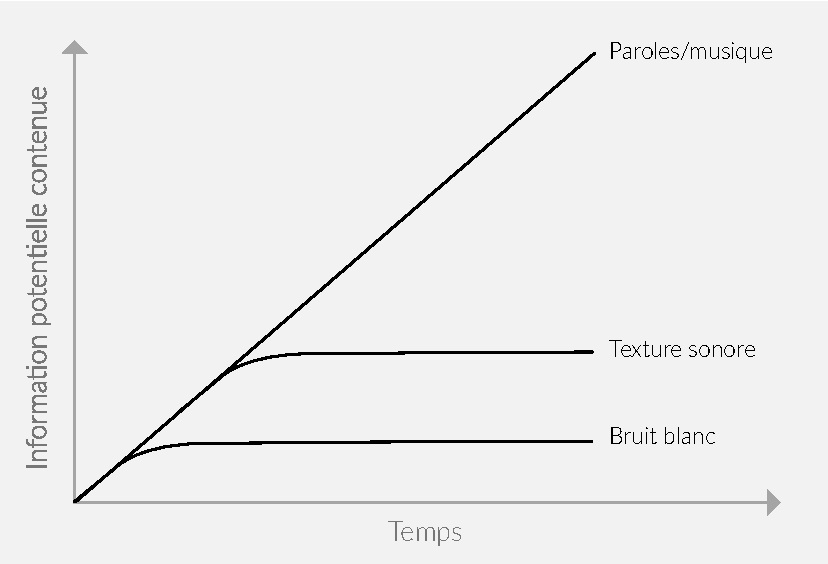
\includegraphics[width=.8\linewidth]{gfx/texture}
        \caption[Information potentielle contenue dans les séquences d'événements, les textures, et le bruit]{Information potentielle contenue dans les séquences d'événements, les textures, et le bruit. D'après \citep{saint1995classification}}\label{fig:texture}
\end{figure}

\subsection{Percevoir les textures}

Contrairement aux événements sonores, la texture est un objet simple, dont le traitement cognitif ne requiert pas une analyse poussée. 

Cela a été mis en évidence par Josh H. McDermott et ses-co auteurs \citep{mcdermott2011sound,mcdermott2013summary}. S'inspirant du fonctionnement de l'oreille humaine, et notamment des processus auditifs intervenant depuis la cochlée, jusqu'au thalamus, ils ont pu établir un modèle permettant de re-synthétiser des textures sonores en ne se servant que de statistiques simples, calculées à partir de représentations temps-fréquence de signaux de textures enregistrés. 

Dans une première expérience \citep{mcdermott2011sound}, la capacité des sujets à identifier les textures synthétisées a été testée. Les résultats ont montré que les sons de synthèse étaient aussi bien identifiés que les sons enregistrés. McDermott démontre ainsi qu'une information résumée sous la forme de statistiques, est utile, d'un point de vue cognitif, à la reconnaissance. Dans le cas des textures, ces statistiques constituent même l'unique information disponible, le système auditif ayant fait fi de toute autre représentation plus détaillée \citep{nelken2013ear}.

Dans une seconde expérience \citep{mcdermott2013summary}, les sujets ont dû reconnaître, parmi une triade de sons synthétisés, celui produit par une source différente (\ie~un type de texture différent, \cf~Figure~\ref{fig:textureMcder}). Les résultats ont montré que la capacité de discrimination est fonction de la durée des textures. Plus cette dernière est élevée, plus la capacité à discriminer est importante. Ce constat valide les hypothèses formulées par \citep{saint1995classification} sur l'existence d'une période d'attention, nécessaire au cerveau afin de percevoir le stimuli comme une texture. Ces résultats ont aussi montré que le processus de traitement de l'information sonore comprend une prise de décision quant à la nature des stimuli, décision qui va  ensuite influer sur la manière d'analyser l'information montante. L'expérience prouve que cette prise de décision n'a rien d'anodine, car, dans le cas où le cerveau perçoit une texture, il décide sciemment de dégrader l'information, en la résumant de manière statistique.

Le fait qu'un jugement perceptif s'améliore avec la durée des stimuli est un principe bien connu en perception des sons \citep{moore1973frequency}. Une troisième expérience de \citep{mcdermott2013summary} a montré cependant que cette vérité n'était pas toujours vérifiée. Au cours de cette expérience, les sujets, soumis à trois exemplaires d'un même type de texture (\eg~trois sons synthétisés de pluie), dont deux étaient produits à partir des mêmes statistiques extraites, ont du identifier le troisième, issu de statistiques différentes (Figure~\ref{fig:textureMcder}). Les résultats ont montré que la capacité des sujets à discriminer le bon stimulus décroît avec la durée des stimuli. Ce fait, qui peut sembler paradoxal, est une conséquence directe du choix du cerveau de ne traiter les textures que sur la base de statistiques. Partant du principe que le signal sonore est analysé suivant des fenêtres d'intégrations successives \citep{yabe1998temporal,poeppel2003analysis}, plus les stimuli sont longs, plus le système auditif est confiant dans le fait qu'il a à faire à des textures, et plus il tend à conserver une information réduite. La réduction de cette information finit éventuellement par gommer les différences fines qui existent entre les stimuli, ce qui ne permet plus de faire la distinction entre eux.


\begin{figure}[t]
        \myfloatalign
        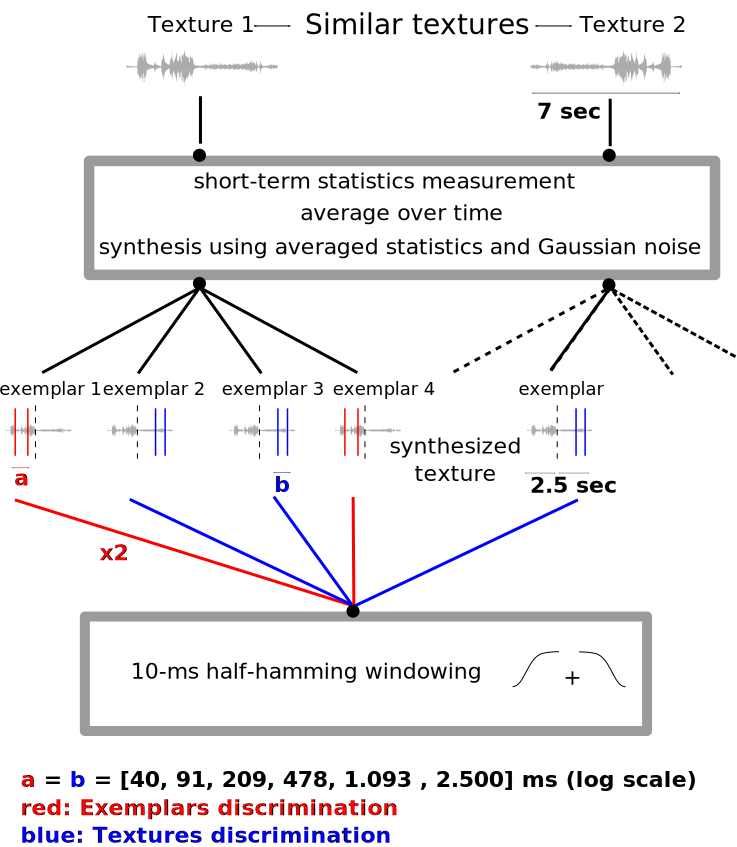
\includegraphics[width=.8\linewidth]{gfx/mcder}
        \caption[Plannification expérimentale de l'expérience de discrimination de textures sonores et d'exemplaires de textures sonores]{Plannification expérientale des expériences de discrimination de textures sonores et d'exemplaires de textures sonores menées par \citep{mcdermott2013summary}}\label{fig:textureMcder}
\end{figure}

Une des avancés majeures de ces études est qu'elles apportent de nouvelles réponses sur la nature des représentations sonores stockées en mémoire. Dans le cas des textures, il s'agirait ainsi de descripteurs bas-niveaux, résumés sous la forme de statistiques simples. Cette découverte fait sens d'un point de vue écologique, car elle respecte le principe d'économie de moyens. Le cerveau, reconnaissant que les caractéristiques des textures n'évoluent pas au cours du temps, ne conserve en mémoire qu'une information condensée, qui lui permet pourtant de traiter des sons potentiellement longs. 

Il a été montré que le cerveau peut stocker bien plus que des statistiques. \citep{agus2010rapid} a mis en évidence qu'un bruit blanc, écouté de manière répétée, pouvait être reconnu encore plusieurs semaines après l'écoute, et ce parmi d'autres bruits blancs. Dans ce cas le cerveau emmagasine bien la totalité du signal acoustique.

\subsection{Période d'attention}

\gl{TODO: déplacer l'expérience en annexe. terminer sur une discussion "texture, un groupe d'evt qui ont perdu leur signification individuelle" + "importance de l'attention span" (dire que ce point a été étudié: introduire l'expérience) + "problème avec le bruit blanc\citep{agus2010rapid}, texture non informatif mais pourtant stockée en totalité par le cerveau"}

\begin{figure}[t]
        \myfloatalign
        \subfloat[]
        {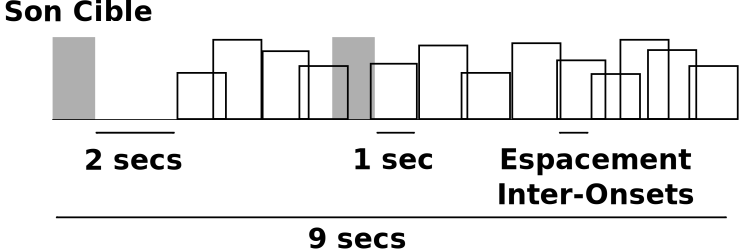
\includegraphics[width=.5\linewidth]{gfx/xpTexture1}\label{fig:xptexturea}}
        \subfloat[]
        {\includegraphics[width=.5\linewidth]{gfx/xpTexture3}\label{fig:xptextureb}}
        \caption[Événement ou texture sonore: influence de la période d'attention]{Événement ou texture sonore: influence de la période d'attention. (a) la nature des stimuli utilisés. (b) le seuil d'espacement moyen permettant de faire la distinction entre une séquence d'événements et une texture}\label{fig:xptexture}
\end{figure}

Nous nous permettons ici de présenter les résultats d'une étude menée dans le cadre de cette thèse, mais déconnectée du sujet principal. 

Nos travaux ont également porté sur cette notion de période d'attention. Comme nous l'avons vu, la texture est un objet composite. En poussant cette vision à l’extrême, une texture peut être vue comme un empilement d’événements sonores, ayant cessés d'être perçus de manière distincte, dès lors qu'ils forment un tout homogène et stable. 

Nous avons suivi cette idée, afin de bâtir un protocole permettant d'analyser la période d'attention. En considérant comme stimuli une mixture d'événements du même type, nous faisons l'hypothèse qu'à partir du moment où le cerveau parvient à isoler un événement de cette mixture, il ne perçoit plus la mixture comme une texture, mais comme une succession d'événements. Inversement, s'il ne parvient pas à distinguer un événement isolé, alors la mixture est perçue comme une texture.

Sur la base de cette hypothèse, une expérience de reconnaissance de type oui/non (\cf~Annexe~\ref{app:xp_texture} pour une description exhaustive de l'expérience) a été montée. Dans cette expérience, chaque stimuli est composé d'un son cible, suivi d'une séquence d'événements enchevêtrés. Tous les événements sont des sons isolés ayant une durée de $1$ seconde. La séquence dure 6 secondes (\cf~Figure~\ref{fig:xptexturea}). L'objectif pour le sujet est d'indiquer si oui ou non il a entendu le son cible dans la séquence d’événements.

Les séquences donnent à entendre des scènes de trafic. Ces scènes sont simulées en agglomérant des sons de voiture isolés. La simulation est contrôlée par un paramètre réglant l'espacement temporel inter-onset moyen entre les événements. Cinq valeurs d'espacement sont considérées: $0.1$, $0.3$, $0.5$, $0.7$ et $0.9$ secondes. Pour chaque espacement, nous simulons 20 séquences de trafics, chaque sujet devant alors écouter 100 stimuli. La moitié de ces stimuli sont des pièges (\emph{catch trial}), le son cible y étant absent. Nous mesurons les performances des sujets en utilisant la mesure de sensitivité $d'$ (\cf~Annexe~\ref{app:sdt}). Les résultats sont très encourageants. Ils montrent qu'il existe bien un espacement limite à partir duquel la mixture cesse d'être perçue comme une texture. Pour des sons isolés d'une seconde, cet espacement limite est de 0.42 secondes, soit la moitié de la durée des événements utilisés (\cf~Figure~\ref{fig:xptextureb}).

\begin{figure}[t]
        \myfloatalign
        
\includegraphics[width=\linewidth]{gfx/categoSalamon}
        \caption{Taxonomie des sources sonores urbaines, d'après \citep{Salamon14}}\label{fig:catSoundscapeSalamon}
\end{figure}




%*****************************************
%*****************************************
%*****************************************
%*****************************************
%*****************************************

%************************************************
\chapter{Un modèle morphologique de scènes sonores environnementales}\label{ch:psycho_model} % $\mathbb{ZNR}$
%************************************************

\section{Motivations}

\subsection{Analyse sensorielle}

étude de la contribution des sources sonores \\

G1: \citep{bruce2009development,bruce2014effects}; \\
G2: \citep{davies2014soundscape} montre que quand on demande à des participants de simuler un paysage sonore, les simulations font références à ce que les participants s'imaginent être un environnement typique, sans tenir compte de leur propre préférence pour des sons particuliers.

\subsection{Analyse automatique}

\section{Proposition d'un modèle de scènes sonores}

\subsection{Discrétiser l'environnement sonore}

\subsubsection{L'unité de bases: la source sonore}

Les études portant su l'ASA et plus spécifiquement sur les processus de ségrégation montrent que l'humain fait sens de son environnement en isolant les informations relatives aux différentes sources qui composent la scène. Elles montrent notamment que ce groupement intervient très tôt dans la chaîne de traitement, et se base sur des règles génériques innées. \\

\gl{Neurosciene}

De même, la communauté des paysages sonores, adoptant l’approche catégorielle, a également montré que les processus de catégorisation s'appuie également sur la composition sémantique des scènes,\ie~les sources sonores identifiées.

Il semble alors intuitif pour notre modèle de considérer comme élément de base la source sonore. Hors comme nous l'avons vu précédemment (\cf~section~ref{XX}), la notion de source sonore est variable, un même objet pouvant être reconnu suivant plusieurs degré d'abstraction.

\subsubsection{Typologie: source et action}

Avant de pouvoir enregistrer ces sources, il est nécessaire de les identifier. Une approche naïve serait alors d'établir la liste exhaustive de toutes les classes de sources sonores composant l'environnement sonore. Cette approche soulève alors 2 problèmes:

\begin{itemize}
\item Une source sonore peut se décrire avec plusieurs niveaux d'abstraction. Comme nous l'avons vu, identifier et nommé un objet est très lié à notre représentation mentale du monde. Selon la théorie de la catégorisation, l'organisation catégorielle de nos représentations se déploient, entre autre, selon un axe verticale, relatif au niveau d'abstraction considéré pour catégoriser un objet perçu. Ainsi, si 2 individus entendent un même son de voiture, il est possible que le premier le nomme ``\,voiture\,'' et le deuxième ``\,moteur\,''. Le dénombrement de l'ensemble des sources pouvant être utilisée par le modèle doit prendre en compte ce fait. Ces sources doivent être regroupée en classes hiérarchisée, afin de bâtir une structure taxonomique.
\item Il n'existe pas de taxonomie standardisé des sources sonores: C'est une tradition des sciences moderne de classer et nommer les différents objets d’intérêt avant de les étudier. Pour ce qui est de la faune ou de la flore, une observation longue et minutieuse ds objets a permis d'élaborer un système de classification standard, permettant d'organiser et trier les différents objets en fonction de leurs propriétés partagées. Les classes d’objets équivalents étant nommé à l'aide d'une terminologie précise. Ce système a permis à la biologie de devenir une science moderne à part entière, et entre autre de mettre à jour le concept de l'évolution des espèces \citep{lecointre2006tree}. Cependant, que ce soit pour les catégories d'odeurs ou les catégories de sons, il n’existe pas de système de classification équivalent \citep{dubois2000categories,niessen2010categories}. Nous isolons trois points qui permettent d'expliquer ce fait
\begin{itemize}
\item \emph{Champ lexical limité}: L'identification et la description d'un son est un processus subjectif très lié au langage. Deux sujets appartenant à deux groupes sociaux différents n'utiliseront pas les mêmes termes pour décrire un même son. Afin d'établir un système de classification standard, il faut prendre une décision quant à la définition précise des termes utilisés pour décrire les phénomènes acoustiques. Cette opération est d'autant plus facile si il existe déjà un consensus autour du sens global des termes. Or, contrairement à la vision, où un vocabulaire de base, largement partagé, est disponible pour décrire les objets (couleur, forme), il s'avère que le champ lexical utilisé pour décrire précisément le monde sonore est très limité (durée, fréquence)  \citep{dubois2000categories}. La plupart des termes couramment utilisés sont  empruntés à d'autres modalités perceptives. On peut par exemple parler de brillance ou de rugosité des sons. La diversité des termes descriptifs, ainsi que l'absence de consensus sur ce qu'ils désignent, rend difficile la production d'une classification standardisée des sons.
\item \emph{Influence du contexte}: Comme vu à la section~\ref{sec:ch3_identification et Contexte}, l'identification et la description d'une source sont dépendantes du contexte, \ie~de la nature des sources cooccurrentes dans la scènes \citep{ballas1987interpreting,niessen2008disambiguating,gygi2011incongruency}.
\end{itemize}
\end{itemize}

Il apparaît clairement que les classes de sons peuplant notre environnement doivent être organisée autour d'une taxonomie: un système de classe hiérarchisé. Cependant il y a un choix à faire quant à la manière de regrouper les sons à l'intérieur de cette taxonomie.

Comme vu à la section~\ref{XX}, plusieurs études ont montré que la catégorisation de sources sonores s'opère suivant des attributs sémantiques. Parmi ceux-ci, deux reviennent souvent:

\begin{itemize}
\item La source (agent, objet, fonction),\ie~l'objet émettant son.
\item L'action,\ie~le mouvement physique étant la cause du son.
\end{itemize} 

Ces deux attributs fonctionnent de concert. Reprenant l'organisation catégorielle verticale à trois niveaux de Rosch (\cf~section~\ref{sec:ch3_categoEtAbstract}), Guyot et al. \citep{guyot1997} ont proposé un système de catégorisation ou les auditeurs identifient des groupement de sources abstraits au niveau superordonné (``\,Bruit généré par une excitation mécanique\,''), des actions au niveau de base (``\,gratter\,'',``\,frotter\,'') et des sources au niveau subordonné (``\,vaisselles\,'',``\,stylo\,''). Reprenant ce système, \citep{houix_lexical_2012} montre que les sons semblent être catégorisés en premier à partir du type de source, et seulement ensuite sur la base de l'action.


Le couple source-action semble être une bonne base sur laquelle bâtir une taxonomie. Les classes haut-niveaux étant des classes abstraites de sources sonores (``\,véhicule\,''), les classes intermédiaires des classes de sources sonores (``\,voiture\,''), et les classes basses des actions sonores (``\,passage\,''). Pour les classes de bas-niveau, la variabilité intra-classe est alors minimale.

Considérer un couple source-action n'est cependant pas suffisant. Le choix des labels utilisés doit faire l'objet d'une sélection particulière. C'est label doivent être génériques, compréhensible, et décrire de manière non ambiguë les objets de la classe. Afin de les choisir, on peut se référer aux travaux de Gaver \citep{gaver1993world} qui propose une taxonomie phénoménologique des sons, de Niessen~\al \citep{niessen2010categories} qui établissent la liste des catégories sonores les plus utilisées à partir d'une étude bibliographique de 166 papiers, et plus récemment les travaux de Salamon~\al \citep{Salamon14}, qui propose une taxonomie de sons urbains, utilisant également le couple objet-action, et établie sur la base entre autre des travaux de brown~\al \citep{brown2011towards}.

Dans cette partie, nous montrons que  l'utilisation de la nomenclature basée sur le couple action-source nous permet de dénombrer et trier l'ensemble des sons présents dans l'environnement sonore.

Dans un cas pratique, il s'agirait alors, sur la base de la taxonomie établie, d'enregistrer pour chacune des classes  un nombre de sons suffisant. Considérant des environnements dense comme la ville ou la forêt, c'est approche pose des problèmes pratiques de faisabilité évidents. On peut cependant se demander si il est nécessaire d'enregistrer de manière séparé toutes les sources,\eg~doit on additionner plusieurs sons de voix pour simuler un son de foule ? Si oui, la diversité d'enregistrement nécessaire pourrait être considérable, le cerveau humain étant très sensible à la répétition de sons identiques \citep{agus2010rapid}.

Afin de contourner le problème, on peut là encore s’appuyer sur des considérations perceptives afin d'établir, dans un contexte expérimentale donné, quels sons requiert d'être enregistré séparément, et quels groupes de sons peuvent être enregistrer ensemble

\subsubsection{événements, textures et scènes amorphes}

Tout les sons n'ont pas le même intérêt. Typiquement, une voix humaine pourra facilement être isolée du reste des sons concurrents \citep{carlyon2004brain}. De même, un fond sonore de trafiques urbains sera moins informatif que d'autre sons ponctuels et proches~\citep{southworth1969sonic}.

Comme vu à la section~\ref{sec:ch3_catsoundscape}, Maffiolo montrent l'existence de deux processus cognitives distincts dont l'activation dépend de la nature des environnements: pour les scènes amorphes,\ie~sans événement apparent, les scènes sont analysées de manière holistique, alors que des scènes événementielles, \ie~comportant des événements identifiables, sont analysées de manière descriptive, sur la base d'une information sémantique extraite a partir des événements reconnus.

Ces résultats nous amène à penser que les processus de ségrégation dépendent également de la nature structurelle de l'environnement. Lorsqu'un des événements émergent de la mixture, le cerveau traite l'information des différentes sources de manière séparée. Plusieurs flux auditifs sont ainsi générés, \ie~un pour chaque séquence d'événements émis par la même source. A l'inverse, quand le cerveau ne parvient pas à isoler d'événement, la scène est traité globalement,\ie~tout ces éléments étant aggloméré dans un même flux. 

De même, les différents travaux sur les textures sonores (\cf~section~\ref{sec:ch3_eventTexture}), montrent que le cerveau a tendance à tendance à résumer l'information extraite lorsqu'il détecte qu'une séquence n'est  composée que d'un mélange de sons similaires et n'apporte pas d'information au cours du temps. 

Outre les événements sonores, deux autres types de sons semblent pouvoir être isolés:

\begin{itemize}
\item \emph{Scène amorphes}: un son contenant une faible information sémantique et analysé de manière holistique.
\item {Texture sonores}: un son dont les caractéristiques physiques restent stables au cours de temps et traité par le cerveau à partir de statistiques extraites d'une représentation temps-fréquence.
\end{itemize}

Nous pensons qu'il existe des connexions entre les notions de textures/événements, et celles des scènes amorphes/événementielles. Les séquences événementielles peuvent être vues comme des séquences composées soit uniquement d'événements, soit d'événements et de textures, la présence d'événements, porteurs d'une information plus riche, primant sur la nature des processus mis en œuvre. 

De même, les textures et les scènes amorphes sont traitées de manière holistique, à partir de propriétés acoustiques globales pour les scènes amorphes \citep{dubois2006cognitive,maffiolo_caracterisation_1999}, et sur la base d'une information résumée statistiquement pour les textures\citep{mcdermott2013summary}. Toutes deux portent par ailleurs une information limitée \citep{saint1995classification,nelken2013ear}. Cependant, les séquences amorphes sont spontanément décrites par des sujets comme des ``\,fonds sonores\,'' \citep{maffiolo_caracterisation_1999,guastavino2006ideal}, impliquant que ces dernières n'existent que suite à un processus de construction de flux auditifs, alors que les textures sont des objets seulement définis sur la base de leur nature physique. Un exemple de texture souvent cité est le sons du ``\,galop\,'', qui selon le contexte peut très bien se retrouver au premier plan de la scène. 

Considérant cela, nous pensons qu'il est possible de considérer une scènes amorphe comme étant une texture, ses caractéristiques physique demeurant stables au cours du temps, et beaucoup de scènes amorphes (``\,brouhaha de rue\,'', ``\,brouhaha de trafic\,'') étant par ailleurs citées comme étant des textures. Cependant l'inverse, considérer une texture comme une scène amorphe, n'est pas forcément vrai.

Afin de limiter le nombre d'enregistrements nécessaires, il est donc possible d'enregistrer directement des mixtures de sons, à condition que ces dernières puissent être considérée comme des textures, la définition de cette dernière notion englobant les scènes amorphes.

\subsubsection{Discussion}

\subsection{Description du modèle morphologique}


\subsubsection{Séquence de sources sonores}

Dans le modèle proposé, la scène sonore est vu comme une somme de source sonores, ou autrement dit, ``\,un squelette d'événements sur un lit de textures\,'' \citep{nelken2013ear}. 

D'un point de vu pratique, ces éléments sonores sont enregistrés. L'enregistrement d'un son isolé, qu'il s'agisse d'un événement, ou d'une texture est appelé un \emph{sample}. 

\begin{mydef}
Un sample est un enregistrement d'un son isolé, qu'il s'agisse d'un événement, ou d'une texture.
\end{mydef}


Ces samples sont regroupés en classes de sons hiérarchisées, formant une taxonomie. Un exemple d'une partie d'une taxonomie comme utilisé par le modèle est donné figure ~\ref{fig:orgDb}. Les niveaux hiérarchique de la taxonomie sont appelé niveau d'abstraction.  Les classes ayant un niveau d'abstraction élevé illustre un regroupement conceptuels de samples ayant potentiellement des caractéristiques variés (\ie~{Humain}). Plus le niveau de la classe est bas, plus le groupement induit est précis, regroupant des samples similaires (\ie~\emph{voix-adulte-cri}). 

\begin{mydef}
Une classe est une collection de samples, ou une collection de sous-classes, en fonction du niveau d'abstraction considéré.
\end{mydef}

Les classes de niveau d'abstraction élevé sont nommés uniquement à l'aide de terme abstraits désignant de manière global les samples qu'elles regroupent (\eg~\emph{transport}), alors que les classes de bas niveau utilise la nomenclature source-action (\eg~\emph{voiture passe}). Les classes du dernier niveau correspondent à des collections de samples, considéré de facto comme équivalents les uns aux autres.

Chaque classe de son est enfin lié à une piste. Cette dernière peut être vue comme une séquence temporelle où sont positionnés les différents samples. La piste peut être vue comme la contrepartie simulée du flux auditif.

\begin{mydef}
Une piste est une séquence temporelle composée de sample appartenant à une même classe de sons.
\end{mydef}

La construction de la taxonomie (nombre de classes, nombre de niveau d'abstraction), dépend bien évidemment de la tâche considérée. 

\begin{figure}[bth]
        \myfloatalign
        \includegraphics[width=.8\linewidth]{gfx/3}
       \caption{Organisation hiérarchique de la banque de sons isolés utilisée pour la simulation}\label{fig:orgDb}
\end{figure}

\subsubsection{Paramètre}

En suivant la terminologie précédemment introduite, une scène sonore est vue comme une somme de piste. Chaque piste étant une séquence temporelle, dont la structure est dépend d'une série de paramètres. Ainsi, le modèle ne propose pas d’interagir avec un sample en particulier, mais toujours avec une séquence de samples.

Nous isolons trois attributs permettant de contrôler un piste:

\begin{itemize}
\item \emph{Le niveau}: la moyenne/variance des niveaux des samples
\item \emph{L'espacement}: la moyenne/variance des espacements inter-onsets entre les samples
\item \emph{La duré}: le débuts et la fin de la piste
\end{itemize}

Le modèle fait une distinction explicite entre la gestion des pistes d'événements et de textures. En effet, la notion de texture ne peut se comprendre que pour un son continue. Une piste de texture est donc composée de samples concaténé les uns aux autres sans espacement. Ce dernier, dans le cas des textures, est un paramètre imposé, fixé à 0. 

Pour qu'une piste de texture soit ``\,plausible\,'', \ie~qu'on ne détecte pas de discontinuité flagrante, la piste doit être une séquence composé de samples provenant de la même source, et obtenu avec un matériel et des réglages identiques.

\subsubsection{Formalisation du modèle}
 
 Tout au long due nos travaux, nous avons utilisé plusieurs modèles ainsi que différents paramètres afin de simuler des scènes sonores. Nous formalisons dans cette partie une version générale du modèle proposé. Les divers modifications appliquées, quand elles existent, seront indiquées dans les sections adéquates (\cf~section~\ref{xx}).
 
La formalisation présentée vaut uniquement pour les classes d'événements sonores. Nous décrivons par la suite les diverses contraintes qui s'appliquent pour une classe de textures.
 
En considérant $s$, une scène composée de $C$ classes de sons, le modèle de $s$ se définit  comme suit:
 
 \begin{equation}
 s(n)=\sum_{i=1}^{C}p_i(n)
 \end{equation}

avec $n$ un indice temporel discret, et $p_i$ la piste correspondant à la classe $c_i$. La classe $c_i$ est composé de $\vert c_i\vert$ samples $c_{i,m}$, $1<m<\vert c_i\vert$. 

Une piste $p_i$ est définie comme une séquence de $n_i$ samples d'événement $e^k_i(n)$ ($k=(1,2,\ldots,n_i)$), choisis aléatoirement parmi les $\vert c_i\vert$ samples de la classe $c_i$. Considérant $\mathcal{U}(x,y)$, une distribution uniforme d'entiers allant de $x$ à $y$ ($x<y$), on a alors:

 \begin{equation}
 e^k_i=c_{i,\mathcal{U}(1,\vert c_i \vert)}
 \end{equation}

 Pour chaque piste $p_i$, un facteur d'amplitude est tiré aléatoirement à partir d'une distribution normale de moyenne $\mu^a_i$ et de variance $\sigma^a_i$. De même, les espacements inter-onsets sont tirés d'un distribution normale de moyenne $\mu^t_i$ et de variance $\sigma^t_i$. Les indices temporelles de début et de fin de chaque piste sont notés $u_i$ et $v_i$ respectivement. Formellement, une piste $p_i$ se définit comme suit:
 
\begin{equation}
\label{eq1}
p_{i}(n)= \sum_{j=1}^{n_i} \mathcal{N}(\mu^a_{i},\sigma^a_{i})c_{i, \mathcal{U} (1, |c_i|)}(n-n^j_i)
\end{equation}
\begin{equation}
\label{eq2}
n_i^j=n_i^{j-1} + \mathcal{N}({\mu^t_{i},\sigma^t_{i}})
\end{equation}

où $n_i^0=u_i$ par convention. Le signal d'une piste est définit de telle sorte que $p_i(n)=0$ si $n>v_i$. Les paramètres du modèle sont, $\mu^a_i$,  $\sigma^a_i$,   $\mu^t_i$,  $\sigma^t_i$, $u_i$ et $v_i$, et doivent être réglé pour chaque piste $p_i$.


Pour les textures, deux distinctions sont à observer avec le modèle comme définit précédemment: 

\begin{enumerate}
\item L'amplitude du signal ($\mu^a_i$,  $\sigma^a_i$) n'est seulement tirée qu'une seule fois, et la valeur est appliquée à tous les samples.
\item Afin d'éviter tout impression de discontinuité, deux samples de texture sont concaténé en considérant un certain recouvrement. Ce recouvrement est choisi afin de pouvoir appliquer un fondu enchaîné (\emph{cross-fade}) à valeur d'énergie constante entre les samples, et ce afin de donner l'illusion de continuité.
\end{enumerate}


\gl{a revoir avec mathieu et mathias}

\section{Du modèle à la simulation dans le cadre de l'analyse sensorielle: l'outil \emph{Simscene}}

Dans cette section nous présentons une version du modèle précédemment introduit, afin qu'il puisse servir de base à  un outils de simulation, nommé \emph{SimScene}, utilisable dans le cadre de l'analyse sensorielle des scènes sonores.

Nous commençons par proposer un paradigme expérimentale  décrivant le cadre applicatif des épreuves perceptives basées sur la simulation. Nous relions par la suite ce paradigme au modèle de scène sonore, et présentons les fonctionnalité de l'outil \emph{SimScene}.

\subsection{Proposition d'un protocole expérimental basé sur la simulation}


\begin{figure}[bth]
        \myfloatalign
        \includegraphics[width=.8\linewidth]{gfx/1}
       \caption{TODO}\label{fig:paradigmeSimu1}
\end{figure}

\begin{figure}[bth]
        \myfloatalign
        \includegraphics[width=.8\linewidth]{gfx/2}
       \caption{TODO}\label{fig:paradigmeSimu2}
\end{figure}

\begin{figure}[bth]
        \myfloatalign
        \includegraphics[width=.8\linewidth]{gfx/4}
       \caption{Etape de processus de simulation pour l'analyse sensorielle}\label{fig:etapeSimu}
\end{figure}


\subsection{Organisation des sons isolées}
\label{db_ui}



\subsection{Sélection des sons isolés}

\subsection{Processus de simulation et paramètres de contrôle}

\section{Du modèle à la simulation dans le cadre de l'analyse automatique}

%*****************************************
%*****************************************
%*****************************************
%*****************************************
%*****************************************


\cleardoublepage
\ctparttext{preamble text here.}
\part{Analyse perceptive des scènes sonores environnementales}
%************************************************
\chapter[Application à l’étude perceptive des environnements sonores urbains]{Application du modèle morphologique à l’étude perceptive des environnements sonores urbains}\label{ch:psycho_xp}
%************************************************

\section{Introduction}

Comme nous l'avons motivé à la section~\ref{XX}, il y a un besoin dans la communauté des soundscape d'étudier l'influence séparée des différentes sources sonores sur la qualités perçues de l'environnement. La simulation offre une solution intéressante, car elle nous permet d'obtenir des scènes sonores dont nous connaissons tous les paramètres structuraux, en particulier les caractéristiques distinctes des différentes sources.

Afin de montrer les potentialités découlant de l'utilisation de scènes simulées dans les études perceptives, nous choisissons comme cadre applicatif le problème de l'agrément perçu dans les environnements sonores urbains. 

Cette section présente les résultats d'une série de quatre expériences qui visent à étudier les éléments sonore qui influent sur l'agrément perçu. Toutes ses expériences s'appuient sur la simulation. La première est l'expérience de simulation à proprement parler\ie~où les sujets doivent créer les environnements. Les autres sont des épreuves de notations ou de tri classiques, utilisant les scènes simulées comme stimuli. 

Nous présentons dans la liste suivante un rapide résumé de chacune des expériences:

\begin{enumerate}
\item \emph{Expérience de simulation}: Dans cette expérience, les sujets doivent simuler 2 environnements sonores urbains chacun, en utilisant l'outil et le protocole de simulation décrits à la section~\ref{XX}. le premier environnement doit être idéale/agréable, et le deuxième non-idéale/désagréable.
\item \emph{Évaluation de l'agrément}: Les sujets doivent évaluer l'agrément des scènes simulées sur échelle sémantique.
\item \emph{Évaluation de l'agrément après modification des scènes}: Comme pour l'expérience précédente, les sujets doivent évaluer l'agrément des scènes simulées sur échelle sémantique. Cependant les scènes ont été modifiées, privées de certaines classes de sons identifiées comme ayant un impact sur l'agrément perçu. 
\item \emph{Catégorisation libre}: Les sujets doivent catégoriser les scènes sonores simulées.
\end{enumerate}

Les expériences 1 et 2 sont toutes deux décrites dans la section~\ref{sec:xp1_2}. Les expériences 3 et 4 sont elles décrites respectivement dans les sections~\ref{sec:xp3} et~\ref{sec:xp4}  \\


Tout au long de la présentation des résultats de ces expérience, nous conservons deux objectifs:

\begin{itemize}
\item \emph{expérimental}: Montrer les possibilités offertes par l'utilisation de scènes simulées  dont nous connaissons précisément la partition~\ref{XX} dans le cadre d'études sensorielles ayant trait à la perception des sons.
\item \emph{applicatif}: Étudier quels sont les éléments qui participent de l'agrément dans les environnements sonores urbains. 
\end{itemize}

\section{Contribution spécifique des sources sonores sur l'agrément perçu}
\label{sec:xp1_2}

\subsection{Objectif de l'expérience}

Il s'agit ici d'étudier l'influence de sources sonores spécifiques sur l'agrément perçu des environnements sonores urbains. Pour ce faire, une étude perceptive en deux temps est planifiée (\Cf~Figure~\ref{fig:xp1_2}):

\begin{itemize}
\item \emph{Simulation}: Dans cette première expérience, les sujets doivent simuler deux environnements, le premier étant idéale/agréable (i-scène) et le deuxième non-idéale/désagréable (ni-scène).
\item \emph{Évaluation}: Dans cette deuxième expérience, un deuxième groupe de sujets doit évaluer l'agrément des scènes simulées.
\end{itemize}

L'analyse que nous faisons s'appuie sur les données produites par les deux expériences.

Les objectifs de l'expérience d'évaluation sont doubles:

\begin{enumerate}
\item Évaluer de manière plus fine l'agrément des i- et ni-scènes, afin notamment de pourvoir évaluer pour une même type d'environnement (i ou ni) comment les différentes sources influent sur l'agrément.
\item Détecter la présence de cas extrêmes ou ambigus (\emph{outlier}) dans les scènes simulées. Pour le reste de notre étude, la distinction imposée entre les environnements i et ni sert de référence. Il nous faut donc garantir qu'il n'y ait pas d’ambiguïté entre les cas extrêmes des i- et ni-scènes, \ie~que la note d'agrément la plus basse des i-scènes reste supérieure à la note la plus haute des ni-scènes.
\end{enumerate}

\begin{figure}[t]
        \myfloatalign
        \includegraphics[width=.8\linewidth]{gfx/5-eps-converted-to}
        \caption{Planification expérimentales des éxperiences de simulation et d'évaluation de l'agrément}\label{fig:xp1_2}
\end{figure}

Cette expérience a fait l'objet d'une expérience pilote \citep{lafay2013atiam,lafay2014new}.

\subsection{Banque de données de sons isolés}

Dans cette section, nous présentons le processus de sélection et d'acquisition des sons isolés utilisés comme matériaux de base lors de la simulation des environnements sonores urbains. La banque de données est identique à celle utilisée dans le cadre de l'expérience pilote \citep{lafay2013atiam,lafay2014new}. Nous invitons le lecteur à se référer à la section~\ref{sec:db_ui} pour une description détaillée sur la manière dont les sons sont organisés dans la banque de données, ainsi que de l'interface permettant de les sélectionner. 

\subsection{Typologie des sources sonores présentes dans l'environnement urbain}

Dans le but de créer un corpus de sons isolés de référence pour la simulation, nous avons réalisé une typologie des sons environnementaux urbains. Dans un premier temps, les éléments présents dans cette typologie sont issus d’une étude bibliographique.

Nous recherchons les sources et ambiances sonores les plus souvent citées dans la littérature. Notre étude porte sur 16 articles ou thèses. Chacun d’eux traite de la manière dont nous discriminons les paysages sonores urbains. Plusieurs approches sont possibles, nous en avons relevés 3 :

\begin{itemize}
\item 9 articles abordent le problème par une approche perceptive, soit en identifiant ou répertoriant des catégories de sources sonores, soit en étudiant l'impact de classes de sons spécifiques sur la perception de l'environnement : \cite{maffiolo_caracterisation_1999,raimbault2002simulation,guastavino_etude_2003,defreville2004aactivity,raimbault2005urban,dubois2006cognitive,devergie_relations_2006,guastavino2006ideal,niessen2010categories}
\item 3 articles proposent une classification morpho-typologique, divisant l’environnement sonore urbain en ``\,zones sonores\,'' possédant une identité acoustique forte selon la configuration et la pratique du site : \cite{maffiolo_caracterisation_1999,beaumont2004pertinence,polack2008perceptive}
\item 2 articles répertorient et classifient les sources sonores d’un point de vu expert : \cite{leobon_analyse_1986,brown2011towards}
\end{itemize}

La nature des classes est établie par rapport aux catégories perceptives ou classes de sons les plus souvent citées dans ces papiers. A  partir des éléments relevés, nous établissons deux taxonomies : une pour les événements (\cf~Figure~\ref{fig:taxonomie}.a), et une pour les textures (\cf~Figure~\ref{fig:taxonomie}.b). Comme évoqué à la section~\ref{sec:db_ui}, la structure taxonomique de ces deux ensembles s'inspire grandement de l'axe verticale de l'organisation catégorielle comme proposée par E. Rosch (\Cf~section~\ref{XX}), \ie~plus le niveau d'abstraction de la classe est élevé, plus la description de la classe est précise et plus les source sonores appartenant à la classe sont semblables (\Cf~Figure~\ref{fig:orgDb}). Pour les événements, nous considérons 4 niveaux d'abstraction allant des classes les plus globalisantes (niveau d'abstraction 0) au classes les plus spécifiques (niveau d'abstraction 3). Pour les textures nous ne considérons que 3 niveau d'abstraction.

Nous notons que la typologie ainsi obtenue est très similaire à une autre typologie de sources sonores présentes en milieu urbain effectuée postérieurement \citep{Salamon14}. \\

\gl{Vérifier les articles que Salamon utilise pour établir sa typologie}

\begin{figure}[bth]
        \myfloatalign
        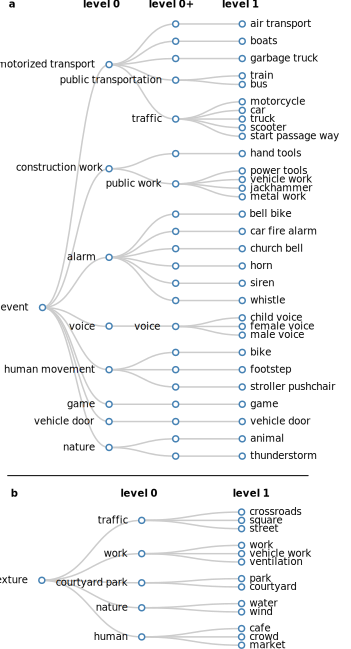
\includegraphics[width=.5\linewidth]{gfxHierarchy/taxonomy}
       \caption[Taxonomies des classes de sons utilisées pour la simulation des environnements sonores urbains]{Taxonomies des classes de sons utilisées pour la simulation des environnements sonores urbains pour (a) les événements sonores et (b) les textures sonores. Nous présentons ici uniquement les niveaux d'abstraction 0 et 1. Un niveau intermédiare, nommé $0+$ et utilisé pour l'analyse est également introduit.}\label{fig:taxonomie}
\end{figure}

\subsection{Acquisition des sons isolés}

Sur la base des typologies précédemment établies, nous avons collecté 483 sons, dont 381 des événements et 102 des textures.

Parmi les sons d'événements :

\begin{itemize}
\item 260 sont issus d’enregistrements
\item 89 sont issus de la banque de sons \emph{SoundIdeas}\footnote{Pour plus de détails sur \emph{SoundIdeas} voir :\url{ http://www.sound-ideas.com/}}
\item 32 sont issus de la banque de sons \emph{Universal SoundBank}\footnote{Pour plus de détails sur \emph{Universal SoundBank} voir : \url{http://www.universal-soundbank.com/}}
\end{itemize}

Parmi les textures:

\begin{itemize}
\item 72 sont issus d’enregistrements
\item 23 sont issus de la banque de sons \emph{SoundIdeas}
\item 7 sont issus de la banque de sons \emph{Universal SoundBank}
\end{itemize}

Tous les enregistrements ont été effectués à l’aide d'un micro canon \emph{AT8035}\footnote{\Cf~\url{http://eu.audio-technica.com/fr/products/product.asp?catID=1&subID=6&prodID=1845}} relié à un enregistreur \emph{ZOOM H4n}\footnote{\Cf~\url{http://www.zoom.co.jp/english/products/h4n/}}. L’utilisation du micro canon nous permet d’isoler les événements sonores du magma urbain. Inversement, pour les textures, il nous permet d’éviter les événements sonores proches du preneur de son, chose impossible avec un micro omnidirectionnel. Nous pouvons ainsi pointer des "zones sonores", en nous tenant à une certaine distance de ces dernières afin de capter uniquement le brouhaha émanant de la zone ciblée.

Tous les sons ont été normalisés au même niveau $RMS$ \footnote{Le niveau $RMS$, de l'anglais \emph{Root Mean Square} désigne la valeur efficace d'un signal. Formellement, le niveau $RMS$ $x_{RMS}$ d'un signal $x=(x_1,x_2,\ldots,x_n)$ s'obtient en calculant la moyenne quadratique de ce dernier $x_{RMS}=\sqrt{\dfrac{1}{n}\sum\limits_{i} x_i^2}$} de $-12$ $dB$ (FS) \footnote{$dB$ (FS) est le sigle anglais désignant une valeur en décibel relative à la pleine échelle (\emph{relative to Full Scale}), \ie~le rapport entre le niveau du signal et sa valeur maximale. Dans notre cas, ce niveau pleine échelle est de 1 Volt.}.

\subsection{Planification expérimentale}

\subsubsection{Épreuve de simulation}

\textbf{Procédure} \\

Les sujets doivent simuler deux environnements sonores urbains, chacun d'une durée de 1 minute.  Pour les deux simulations, les sujets doivent se conformer aux consignes suivantes.

\begin{itemize}
\item Première simulation : Simuler un paysage sonore \textbf{urbain plausible} qui selon vous est idéal (où vous aimeriez vivre).
\item Deuxième simulation : Simuler un paysage sonore \textbf{urbain plausible} qui selon vous est non-idéal (où vous n'aimeriez pas vivre).
\end{itemize}

Tous les sujets commencent par simuler l'environnement idéal. Les sujets ne prennent connaissance de la deuxième consigne qu'à la fin de la première simulation.

Les sujets son totalement libres dans le choix des sons, et des paramètres. Il doivent cependant se conformer à deux contraintes:

\begin{itemize}

\item Les sujets doivent mimer un auditeur statique.
 
\item Les environnements simulées doivent être plausibles, \ie~les sujets ne doivent pas simuler de situation physiquement irréalistes. L'exemple suivant d'une situation physiquement irréaliste est donné aux sujets: 

\begin{quote}
Un chien aboyant toutes les 10 millisecondes.
\end{quote}

\end{itemize}

Avant de commencer la première simulation, les sujets doivent réaliser un petit tutoriel de 20 minutes, afin de se familiariser avec le logiciel de simulation.

L'expérience est prévue pour durer 2h30. \\


\gl{description détaillée des étapes de simulation} \\


\textbf{Apparatus} \\

Tous les sujets passent l'expérience sur des machines identiques (\gl{description des machines}). L'audio est présenter en stéréophonie, par le biais de casques audio. Pendant le tutoriel,les sujets doivent ajuster le niveau sonore à un volume confortable. Ils ne peuvent le modifier par la suite.

Tous les sujets réalisent l'expérience simultanément. Ils sont répartis de manière égale dans trois pièces identiques, toutes possédant un environnement calme. Ils n'ont pas le droit de s'adresser la parole pendant l'expérience.

Trois expérimentateurs, un dans chaque pièce, sont présents durant la totalité de l'expérience, afin de contrôler le bon déroulement de cette dernière, et de répondre à d'éventuelles questions des sujets.  \\

\textbf{Participants} \\

44 étudiants (14 femmes) de L’École Centrale de Nantes ont participé à l'expérience. Ils ont tous un peu près le même âge (moyenne: 21.6, écart-type: 2). Tous les sujets ont vécu dans la même ville (Nantes), au minimum pendant les deux dernières années précédant l'expérience.

Dû a une incompréhension des consignes, ou à l'impossibilité de finir dans les temps, 4 sujets ne sont pas pris en compte pour l'analyse. 40 sujets ont réalisés l'expérience avec succès, nous fournissant ainsi 80 scènes sonores simulés, 40 idéals, et 40 non-idéals.

\subsubsection{Épreuve d'évaluation de l'agrément}

\textbf{Procédure} \\

Les sujets doivent évaluer l'agrément des 80 scènes sonores simulées. Dû à des contraintes de temps, les sujets n'évaluent que 30 secondes des scènes simulées (à l'origine d'une durée de 1 minute). Ces 30 secondes sont extraites à partir de la 15ème et jusqu'à la 45ème seconde des scènes simulées de 1 minute.

L'évaluation s'effectue sur une échelle sémantique bipolaire de 7 points allant de -3 (non-idéal/très désagréable) à +3 (idéal/très agréable). Avant de noter une scènes, les sujets doivent obligatoirement écouter les 20 premières secondes de cette dernière. Après la notation, ils sont libre de passer à la scènes suivante, avant la fin des 30 secondes.

Pour chaque sujet, les scènes sont présentées dans un ordre aléatoire. Les dix premières scènes permettent au sujet d'ajuster ses notes. Elles sont obligatoirement composées de 5 scènes idéales et 5 non-idéales. Ces dix premières scènes sont rejouées à la fin de l'expérience, et seules les notes données à la deuxième occurrence sont prises en compte. \\

\textbf{Apparatus} \\

Tous les sujets passent l'expérience sur des machines identiques (\gl{description des machines}). L'audio est présenté en stéréophonie, par le biais de casques audio semi-ouvert \emph{Beyer-Dynamic DT 990 Pro}. Toutes les scènes sonores ont été re-simulée sur la base des partitions (\gl{citer section décrivant le terme partition}) obtenues lors de l'expérience de simulation. Le niveau sonore de sortie est identique pour tous les sujets.

Tous les sujets réalisent l'expérience simultanément, dans un environnement calme. Ils n'ont pas le droit de s'adresser la parole pendant l'expérience.

Un expérimentateur est présent durant la totalité de l'expérience, afin de contrôler le bon déroulement de cette dernière, et de répondre à d'éventuelles questions des sujets.  \\

\textbf{Participants} \\

10 étudiants (2 femmes) de L’École Centrale de Nantes ont participé à l'expérience. Aucun d'entre eux n'a réalisé l'expérience de simulation. Tous les sujets ont un peu près le même âge (moyenne: 23.1, écart-type: 1.8). Tous les sujets ont vécu dans la même ville (Nantes), au minimum pendant les deux dernières années précédant l'expérience.

Tous les sujets ont réalisés l'expérience avec succès.

\subsection{Données et méthodes d'analyses}

\subsubsection{Nature des données analysées}

Chaque scène est décrite par un groupe de descripteurs. C'est sur la base de ces descripteurs que nous pratiquons l'analyse. Un résumé des descripteurs, ainsi que des acronymes les désignant est présenté dans le Tableau~\ref{XX}.

Les descripteurs sont calculés sur chaque scène sonore. Nous considérons trois types de descripteurs:

\begin{itemize}
\item \emph{Perceptif}: Il s'agit de l'agrément perçu des scènes simulées, évalué sur une échelle sémantique 7 points. Nous notons $A$ l'agrément moyen d'une scène, obtenu en moyennant les notes de tous les sujets. Considérant le faible nombre de sujets, nous faisons le choix dans cette étude de ne pas normaliser les notes d'agrément.
\item \emph{Sémantique}: Il s'agit d'un vecteur booléen noté $S=(x_1,x_2,\ldots,x_n)$ indiquant les classes de sons présentes dans la scènes. Chaque point $x$ de ce vecteur correspond à une classe de son particulière: $x=1$ si la classe est présente dans la scènes, et $x=0$ autrement. La dimension $n$ des vecteurs dépend ainsi du niveau d'abstraction considéré, \eg~pour le niveau d'abstraction 1, qui comprend $44$ classes de sons, cette dimension sera de $n=44$.
\item \emph{Structurel}: Les descripteurs structurels sont calculés à partir des partitions et des signaux des scènes simulées. Trois descripteurs structurels sont envisagés:
\begin{itemize}
\item \emph{Diversité} ($DIV$) : Il s'agit d'un scalaire représentant la diversité des classes sonores utilisées pour simuler une scènes. Nous calculons $DIV$ en comptant le nombre de classes de sons distinctes utilisées pour une simulation. Ce nombre dépend du niveau d'abstraction considéré. Considérons les 2 sous classes du niveau d'abstraction 2 \emph{passage de voiture} et \emph{démarrage de voiture}, toutes deux appartenant à la classe \emph{voiture} du niveau d'abstraction 1, nous comptons 2 classes pour la diversité des niveaux d'abstraction 2 et 1, et seulement 1 pour les niveaux d'abstraction 0 et 1.
\item \emph{Densité} ($D$) : Il s'agit d'un scalaire représentant le nombre de source sonore présentes en moyenne. Pour obtenir $D$, nous calculons le logarithme du nombre d'éléments sonores par fenêtre de 125 millisecondes (sans recouvrement) et moyennons au cours du temps. Le calcul de $D$ peut inclure toutes les sources sonores de la scènes, ou seulement une partie. Dans ce cas, les fenêtres ne contenant pas de sources sonores ne sont pas prises en compte. Nous notons $DE$ et $DT$ les densités calculées en considérant séparément les source d'événements et de textures sonores respectivement.
\item \emph{Niveau Sonore} ($L$) : Pour représenter le niveau sonore, nous nous inspirons du la mesure $L_{Aeq}$. Dans notre cas, il s'agit d'un scalaire, calculé sur le signal en volt et non en pression, et donné en décibel en prenant un référentiel de 1 Volt. Le niveau est obtenu en calculant toutes les secondes la moyenne quadratique du signal, et en moyennant sur la durée de la scène. Un filtrage de type A est opéré avant le calcul des moyennes quadratiques. D'autre descripteurs inspirés eux aussi de descripteurs acoustiques classiques ($L_{Amin}$, $L_{Amax}$, $L_{A10-90}$), et utilisant un opérateur autre que la moyenne (minimum, maximum, les 10-90ème quantiles) pour intégrer les fenêtres de 1 seconde  ont été testés. Mais ces derniers présentant tous une corrélation élevé avec $L$ ($r_{pearson}\geq0.76$, $p<0.01$), nous conservons uniquement ce dernier comme descripteur objectif du niveau sonore.
\end{itemize}
\end{itemize}

\gl{tableau résumé des descripteurs}

\subsubsection{Méthodologie et Outils statistiques}
\label{sec:ch5_methodoEtStat}

L'objectif de l'étude est d'évaluer l'impact spécifique des différentes sources sonore sur l'agrément perçue via l'utilisation de scènes simulées. Afin de répondre à cette question, nous divisons l'étude en 6 sous-objectifs:

\begin{itemize}
\item \emph{Étude qualitative} : Afin de vérifier la validité écologique de 1) la banque de données et 2) l'interface de sélection, nous réalisons une étude qualitative des commentaires libres des sujets effectués après l'épreuve de simulation.
\item \emph{Étude comparative entre les descripteurs structurels} : Il s'agit ici d'évaluer si la distinction affective imposée entre les i- et ni-scènes a impacté de manière significative la nature des scènes, \ie~si il existe des différences significatives entre les descripteurs structurels et/ou l'agrément perçu. La significativité est évaluée à partir d'un test de Student à échantillons apparié (\Cf~Annexe~\ref{app:statuni}).
\item \emph{Influence des descripteurs structurels sur l'agrément perçu}: Nous adoptons ici une méthodologie couramment utilisée dans l'approche dimensionnelle. Pour évaluer l'impact potentiel des descripteurs structurels sur l'agrément perçu, nous étudions l'existence de corrélation linéaire entre entre ces deux types de descripteur. Pour mesurer la corrélation, nous utilisons le coefficient de Pearson (\Cf~Annexe~\ref{app:statuni}).
\item \emph{Étude comparative entre les descripteurs sémantiques}: Il s'agit ici d'apprécier si la distinction affective imposée a eu un impact sur la composition des scènes en terme de sources sonores. Plus précisément, il s'agit d'observer si il existe des classes de sons qui ont été particulièrement utilisées pour simuler un type d'environnement. Nous utilisons le V-test afin de tester si la présence d'une classe de son est typique d'un environnement (i ou ni) en particulier. Ces classes typique sont nommées les marqueurs sonores.\\
 \gl{Décrire ici le V-test}
\item \emph{Étude des espaces de représentations induits par les descripteurs sémantiques}: Dans cette analyse, nous étudions si une représentation basée uniquement sur la présence ou l'absence des classes de sons permets de séparer les deux types d'environnements. Pour ce faire nous considérons l'espace induit par les descripteurs sémantiques $S$. $S$ étant un vecteur booléen, nous calculons les distances entre les scènes à partir de la distance de \emph{hamming}. Considérant les deux vecteurs $S_1=(x_{1,1},x_{1,2},\ldots,x_{1,n})$ et $S_2=(x_{2,1},x_{2,2},\ldots,x_{2,n})$ de dimension $n$, avec $x={0,1}$, la distance de \emph{Hamming} $d_{ham}$ mesure le pourcentage de coordonnés qui diffèrent entre les deux vecteurs. 


\begin{equation*}
d_{ham}(S_1,S_2)=\dfrac{1}{n}\sum_{i=1}^{n} (x_{1,i} \bigoplus x_{2,i})
\end{equation*}

où $\bigoplus$ désigne l'opérateur du \emph{ou-exclusif}. Plus la composition des deux scènes est similaire, et plus ces deux scènes seront proches. L'utilisation de la distance de \emph{Hamming} permet de prendre en compte de manière égale les classes présentes et absentes. Pour mesure la capacité intrinsèque de l'espace à séparer les i- et ni-scènes nous utilisons une métrique de \emph{clustering} nommé précision au rang $k$ ($p@k$). Pour calculer la $p@k$, on regarde d'abord pour chaque item, le taux d'items partageant le même label parmi ses $k$ plus proche(s) voisin(s). La $p@k$ est alors la moyenne des taux pour tous les items.

\item \emph{Influence spécifique marqueurs sonore sur l'agrément perçu}: Une fois les marqueurs sonores identifiés, nous évaluons une nouvelle fois l'impact potentiel des descripteurs structurels sur l'agrément perçu, mais en ne tenant compte cette fois que des marqueurs sonores pour calculer ces descripteurs.
\end{itemize}

Tous les test de significativité sont effectués avec un seuil critique $\alpha=0.05$. Dans le cas ou la valeur $p\geq0.05$, nous indiquons sa valeur. Dans le cas ou $0.01\leq p<0.05$ nous indiquons seulement $p<0.05$. Dans le dernier cas nous indiquons $p<0.01$.

\subsection{Validité écologique de l'expérience}

\subsubsection{Diversité de la banque de sons}

Nous cherchons dans un premier temps à vérifier que les classes de sons proposées dans la banque de données soient assez diversifiée pour pouvoir simuler un environnent sonore. En analysant les commentaires des sujets portant sur la banque données, nous remarquons que 63\% des sujets ont indiqué avoir été au moins une fois dans l'incapacité de trouver un son, avec un maximum de 4 sons par sujet. Parmi tous les sons manquant relevés, nous avons identifié 26 classes de sons. Parmi ces 26 classes de sons manquantes:

\begin{itemize}
\item  16 sont bien présentes dans la banque de données, l'incapacité des sujets à les trouver n'étant donc pas imputable à la diversité de la base.
\item 1 fait référence a des sons de musique, que nous avons choisis délibérément d'occulter.
\item 9 sont effectivement absentes.  
\end{itemize}

Parmi les 9 classes de sons identifiées comme manquantes, nous observons que ces classes sont très spécifiques (\eg~\emph{voiture de sport} ou \emph{voix d'adolescent}), et peuvent ainsi être remplacé par des classes similaires (\eg~\emph{voiture} ou \emph{voix d'enfant} ou \emph{voix d'adulte}). Nous pensons que ces résultats montrent que la diversité proposée par la banque de sons est suffisante dans le cadre de notre étude.

\subsubsection{Facilité d'utilisation de l'interface de sélection}

En considérant les retours sur l'interface de sélection, nous observons que $32.5\%$ des sujets ont spontanément indiqué que l'interface était un moyen ``\,simple et efficace\,'' de sélectionner des sons sans l'aide de texte. $57.5\%$ des sujets n'ont pas fait mention de difficulté particulière. Seulement $10\%$ des sujets ont signalé avoir rencontré des difficultés avec l'interface, mais sans que ces dernières aient sensiblement affecté la simulation.

Ces résultats tendent à montrer que l'interface de sélection sans texte n'a pas perturbé les sujets outre mesure. Des conclusions similaires ont été obtenues lors de l'expérience pilote \citep{lafay2013atiam,lafay2014new}. \\

\gl{vérifier une dernière fois}

\subsection{Vérification de l'agrément des scènes simulées}

Nous analysons ici l'agrément perçu des $80$ scènes sonores simulées. 

La Figure~\ref{fig:xp2_Aa} affiche l'agrément moyen $A$ pour les i- et ni-scènes. Afin de garantir la cohérence de nos données, nous voulons dans un premier temps nous assurer qu'aucune ni-scène n'ait un $A$ supérieur à celui d'une i-scène. Nous observons la Figure~\ref{fig:xp2_Aa} que quatre scènes ne respectent pas cette contrainte. Ces scènes, ainsi que leurs correspondantes i ou ni, sont supprimées de l'analyse. 36 i-scènes et 36 ni-scènes sont conservées dans la suite de l'analyse.

Dans un second temps nous testons si les sujets ont bien perçu une différence d'agrément entre les i- et ni-scènes. Pour ce faire, nous observons l'agrément moyen de chaque sujet calculé séparément pour chaque type d'environnement (\Cf~Figure~\ref{fig:xp2_Ab}). Il est clair que les i-scènes ont bien été perçues comme significativement plus agréables ($p<0.01$) que les ni-scènes.

\begin{figure}[t]
        \myfloatalign
        \subfloat[]
        {\includegraphics[width=.4\linewidth]{gfxXpUrbanSoundscape/xp2_1}\label{fig:xp2_Aa}}
        \subfloat[]
        {\includegraphics[width=.4\linewidth]{gfxXpUrbanSoundscape/xp2_2}\label{fig:xp2_Ab}}
       \caption[TODO]{TODO}\label{fig:xp2_A}
\end{figure}
 
\subsection{Étude comparative entre les descripteurs structurels}

Dans un premier temps nous nous concentrons sur le niveau sonore. Les figures~\ref{fig:soundlevela},~\ref{fig:soundlevelb} et~\ref{fig:soundlevelc} affichent les distributions des niveaux $L$, $LE$ et $LT$ respectivement. Il existe bien une différence de niveau significative entre les i- et ni-scènes ($L$: $p<0.01$), avec un écart moyen de -7 $dB$ entre ces dernières. Cette différence affecte aussi bien les événements ($LE$: $p<0.01$, écart moyen: -7 $dB$) que les textures ($LT$: $p<0.01$, écart moyen: -6 $dB$). 

Nous vérifions ici sans surprises que le niveau des sources sonore est bien un indicateur d'agrément, les ni-scènes ayant tendance à être plus forte. Par ailleurs, cette différence de niveau affect de manière égale les sources d'événements et de textures sonores. 

Il apparaît que ceux sont les événements qui impactent le plus le niveau global des scènes, l'écart entre $L$ et $LE$ n'étant que de 1 $dB$ pour les i-scènes et les ni-scènes. Cette observation fait écho aux résultats obtenu par Kuwano~\al \citep{kuwano_memory_2003}. Dans un premier temps, les auteurs demandent à un panel de sujet d'évaluer de manière globale une série d'environnements sonores. Dans un second temps, les sujets doivent, pour les mêmes environnements, évaluer le niveau aux instants où ils identifient une source sonore. L'étude montre qu'il n'y a pas de différences significatives entre les jugements globaux et les moyennes des jugements instantanés. On peut penser que nos sujets ont inconsciemment tenu compte de cette réalité perceptive lors de la simulation, en faisant porter le niveau sonore global par des sons courts et bien identifiés, \ie~les événements.

Nous observons enfin que le niveau seul ne permet pas de clairement faire la distinction entre les différents types d'environnement. En effet,  $20\%$ des i-scènes ont un niveau supérieur au niveau minimal des ni-scènes, alors qu'il n'y a pas de recouvrement si l'on considère l'agrément perçu $A$.

Nous considérons maintenant les densités de sources sonores. Les Figures~\ref{fig:densitya} et~\ref{fig:densityb} affichent les distributions de $D$ et $DE$. Que l'on prenne en compte toutes les sources ou uniquement les événements, la densité est significativement plus élevée pour les ni-scènes ($D$: $p<0.01$, $DE$: $p<0.01$). Nous observons un écart moyen de $+0.36$ pour $D$ (soit en moyenne 2.3 sources sonores par fenêtre de plus pour les ni-scènes), et de $+0.32$ pour $DE$ (soit en moyenne 2.1 sources sonores par fenêtre de plus pour les ni-scènes). Si les écarts sont très similaires entre $D$ et $DE$, c'est que la densité des textures ne varie pas de manière significative entre les i- et ni-scènes ($DT$: $p<0.08$), l'écart moyen étant de $+0.17$ (soit en moyenne 0.7 sources sonores par fenêtre de plus pour les ni-scènes), et l'écart médian étant quant à lui nul.

Nous constatons ici que la densité peut être un indicateur de qualité, si l'on considère uniquement les événements sonores. Comme pour les niveaux sonores, la densité ne permet pas de clairement séparer les i- et ni-scènes,  $43\%$ des i-scènes ayant un $DE$ supérieur à la densité d'événement minimale des ni-scènes.

Pour finir, nous nous intéressons à la diversité. Nous affichons sur la figure~\ref{fig:diversity} $DIV$ pour les événements et les textures en distinguant les différents niveaux d'abstractions. Excepté pour le niveau d'abstraction 0, la diversité de classes d'événements sonores est plus élevée pour les ni-scènes ($DIV$ niveau 1,2 et 3: $p<0.01$ ), avec en moyenne 2 classes présentes en plus. Aucune différences significatives n'est observée pour les textures.

Les tendances globales observées tendent à montrer que un environnement sonore non-idéale est plus fort, plus dense et et composé d'une plus grande variété d'événements sonores. Par ailleurs ceux sont les caractéristiques des événements plus celles des textures qui semblent porter la distinction entre les i- et ni-scènes. Cependant, aucun de ces descripteurs ne permets, seul, de faire une distinction nette entre les deux types d'environnements, distinction qui pourtant, est perçue de manière non ambiguë par les sujets. 

\begin{figure}[t]
        \myfloatalign
        \subfloat[]
        {\includegraphics[width=.33\linewidth]{gfxXpUrbanSoundscape/xp_soundlevel_1}\label{fig:soundlevela}}
        \subfloat[]
        {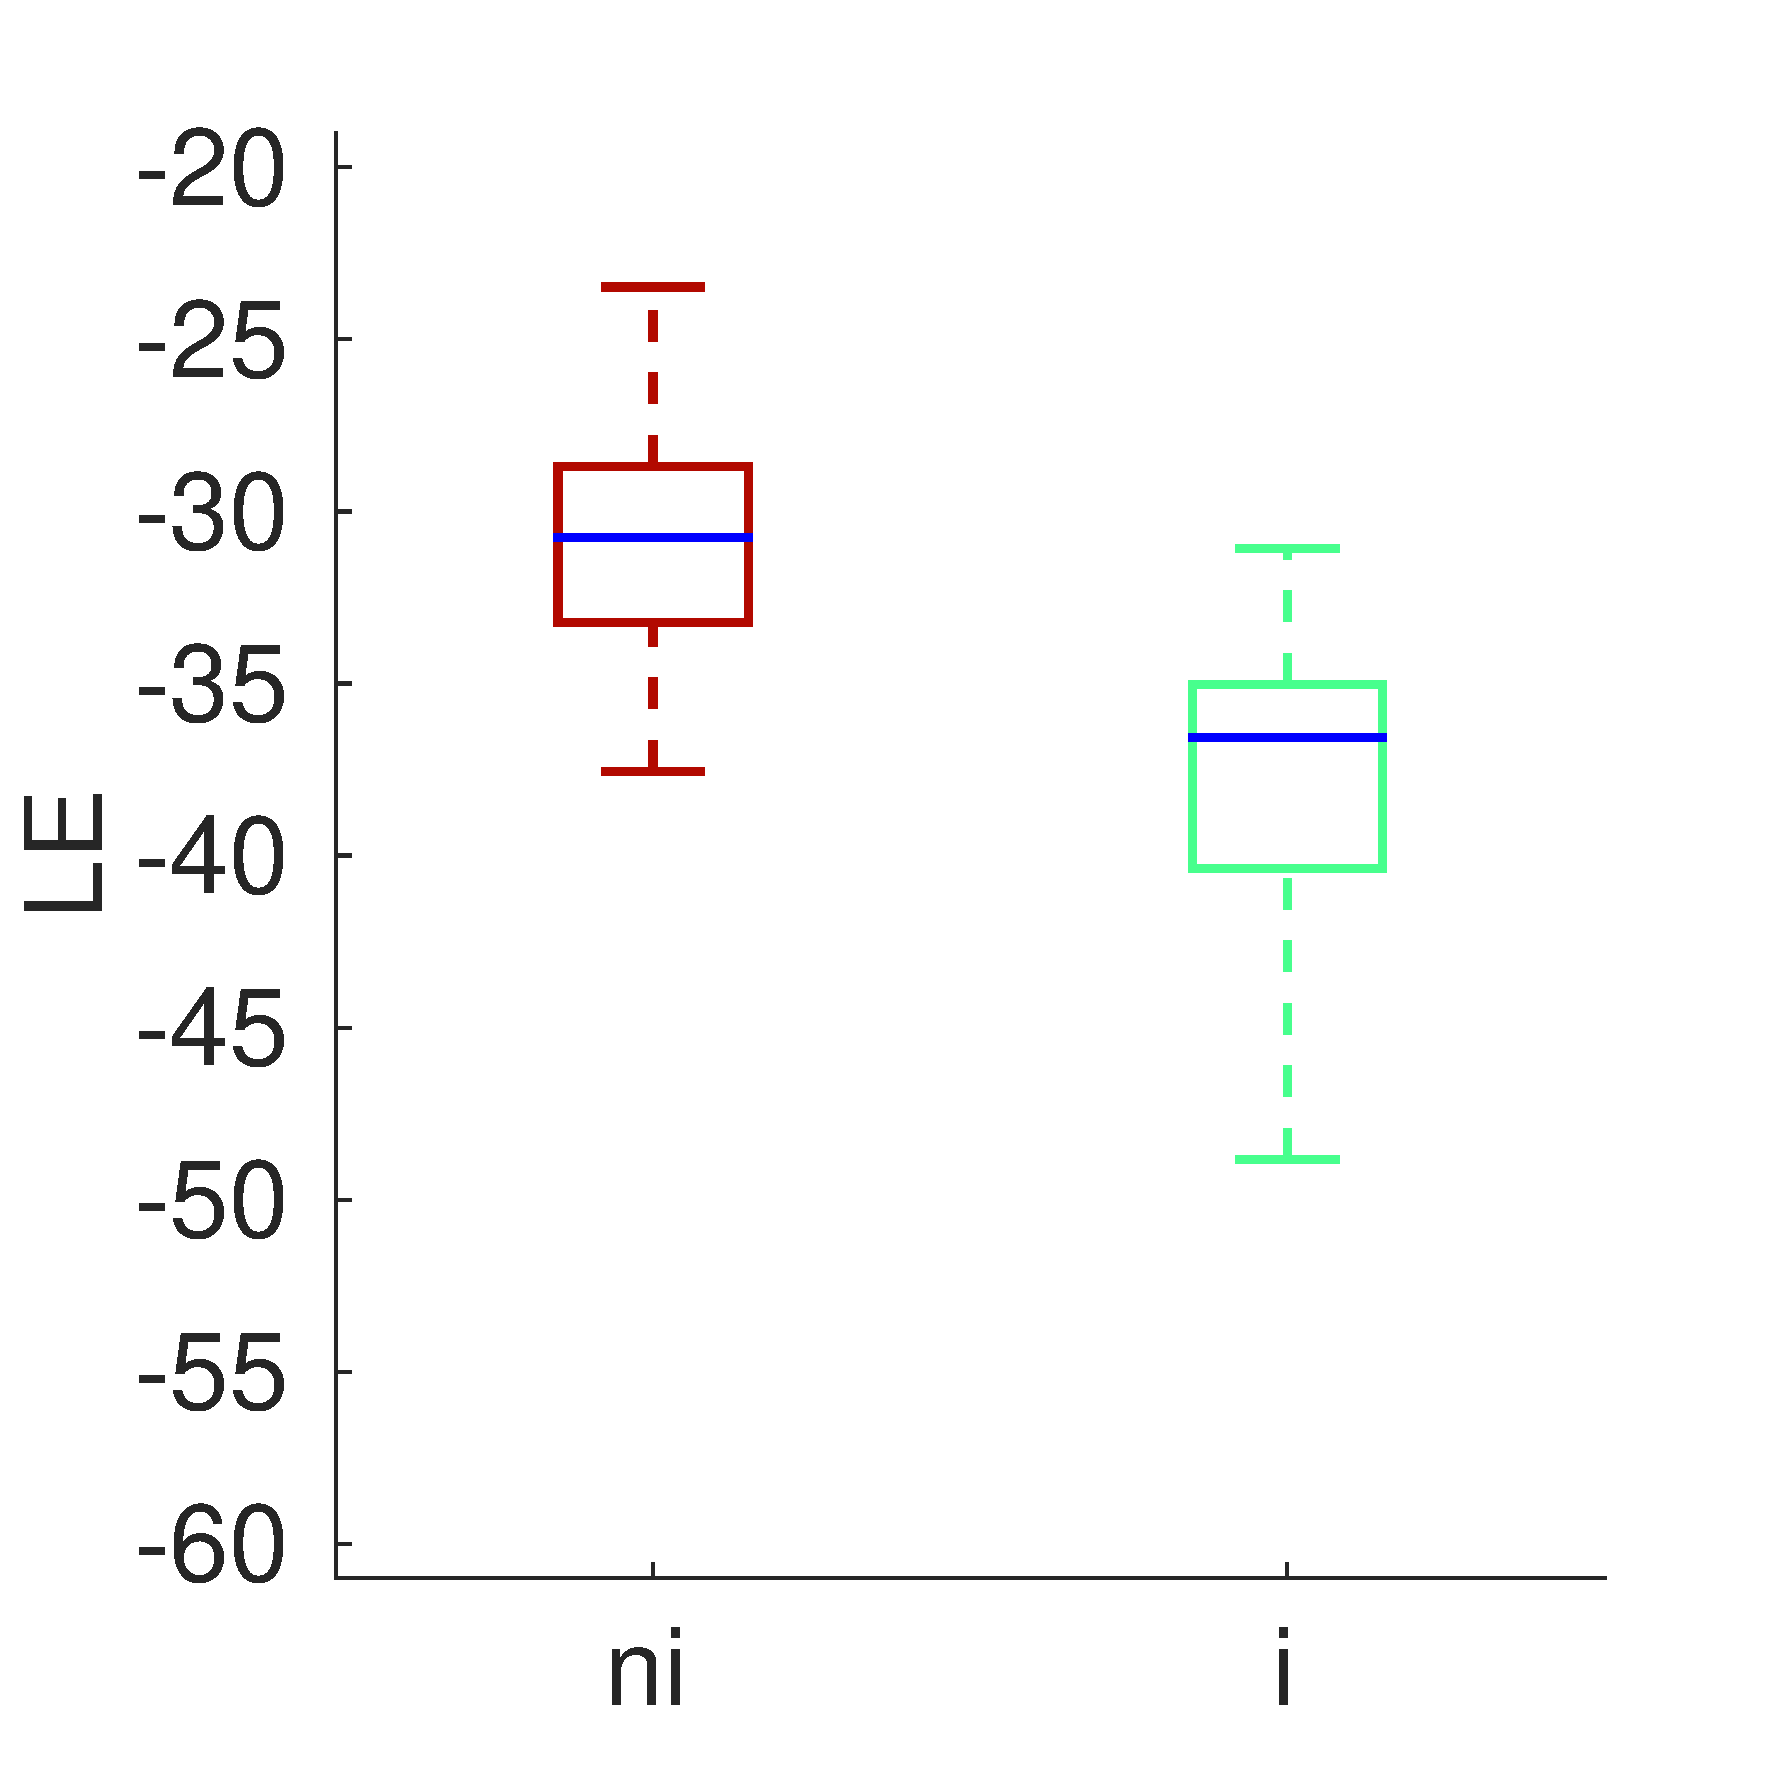
\includegraphics[width=.33\linewidth]{gfxXpUrbanSoundscape/xp_soundlevel_3}\label{fig:soundlevelb}}
        \subfloat[]
        {\includegraphics[width=.33\linewidth]{gfxXpUrbanSoundscape/xp_soundlevel_5}\label{fig:soundlevelc}}\par
        \subfloat[]
        {\includegraphics[width=.33\linewidth]{gfxXpUrbanSoundscape/xp_soundlevel_2}\label{fig:soundleveld}}
        \subfloat[]
        {\includegraphics[width=.33\linewidth]{gfxXpUrbanSoundscape/xp_soundlevel_4}\label{fig:soundlevele}}
        \subfloat[]
        {\includegraphics[width=.33\linewidth]{gfxXpUrbanSoundscape/xp_soundlevel_6}\label{fig:soundlevelf}}
       \caption[TODO]{TODO}\label{fig:soundlevel}
\end{figure}

\begin{figure}[t]
        \myfloatalign
        \subfloat[]
        {\includegraphics[width=.33\linewidth]{gfxXpUrbanSoundscape/xp_density_1}\label{fig:densitya}}
        \subfloat[]
        {\includegraphics[width=.33\linewidth]{gfxXpUrbanSoundscape/xp_density_3}\label{fig:densityb}}\par
        \subfloat[]
        {\includegraphics[width=.33\linewidth]{gfxXpUrbanSoundscape/xp_density_2}\label{fig:densityc}}
        \subfloat[]
        {\includegraphics[width=.33\linewidth]{gfxXpUrbanSoundscape/xp_density_4}\label{fig:densityd}}
       \caption[TODO]{TODO}\label{fig:density}
\end{figure}

\begin{figure}[t]
        \myfloatalign
        \includegraphics[width=.9\linewidth]{gfxXpUrbanSoundscape/xp1_div_1}
       \caption[TODO]{TODO}\label{fig:diversity}
\end{figure}

\subsection{Influence des descripteurs structurels sur l'agrément perçu}
\label{sec:ch5_corrDesStruct}

Nous analysons maintenant dans cette section les relations fines qui peuvent exister entre les descripteurs structurels d'une part et l'agrément perçu d'autre part. Contrairement à la section précédant ou la qualité affective des scènes est représentée de manière binaire (i \vs~ni), nous considérons dans cette section comme descripteur subjectif l'agrément moyen $A$. Il s'agit d'étudier l'existence de potentielles corrélations entre les descripteurs structurels et $A$. Les coefficients de corrélation linéaire calculés entre $A$ \vs~$L$, $LE$, $LT$, $D$, $DE$ et la diversité des classes d'événements ($DIV(E)$) sont présentés dans le tableau~\ref{tab:corrStructA}. Les relations entre $A$ et les descripteurs structurels sont illustrées par les figures~\ref{fig:soundleveld},~\ref{fig:soundlevele} et ~\ref{fig:soundlevelf} pour les niveaux sonores, et les figures~\ref{fig:densityc} et~\ref{fig:densityd} pour les densités. 


Concernant $L$, on observe une forte corrélation négative\footnote{se référer à l'Annexe~\ref{app:corr} pour une explication quant à la manière d'interpréter le coefficient de corrélation dans ce document}  ($r=-0.76$, $p<0.01$) avec $A$, indiquant de fait que plus le niveau sonore est élevé, et plus la scène est désagréable.

Cependant, la figure~\ref{fig:soundleveld} suggère que cette relation ne s'opère pas de la même manière pour les i- et ni-scènes. En effet la corrélation  entre $L$ et $A$ pour les ni-scènes reste élevée ($r=-0.67$, $p<0.01$), mais est inexistante pour les i-scènes. Le fait que la corrélation entre $L$ et $A$, considérant l'ensemble des scènes, soit élevée,  résulte du fait que les i-scènes ont tendance à être moins forte que les ni-scènes, donnant ainsi l'illusion de prolonger la corrélation négative observée pour les ni-scènes.  

On peut donc conclure que $L$ 1) permet bien de faire la distinction entre les i- et ni-scènes, 2) permet de finement caractériser l'agrément perçu des ni-scènes, 3) mais n'est d'aucune utilité comme indicateur de l'agrément perçu  pour des environnements a priori agréables. 

Les mêmes observations sont faîtes si l'on considère $LE$ (\cf~ref{fig:soundlevele}). Pour les textures (\cf~ref{fig:soundlevelf}), bien que l'on observe une corrélation modérée si l'on considère l'ensemble des scènes ($r=-0.51$, $p<0.01$), aucune corrélation n'est relevée si l'on regarde séparément les i-scènes ($r=-0.33$, $p=0.05$) et les ni-scènes ($r=0.09$, $p=0.06$). Là encore on peut penser que la corrélation négative observée pour l'ensemble des scènes est artificielle, venant du fait que le niveau des textures des i-scènes a tendance à être plus bas que celui des ni-scènes. Ainsi, si les événements sonore conservent une certaine capacité de prédiction de l'agrément pour les ni-scènes, le niveau des textures n'apporte lui que peu d'information, qu'importe l'environnement considéré.

Considérant l'ensemble des scènes, nous observons un corrélation négative faible pour $D$ ($r=-0.41$, $p<0.01$) et $DE$ ($r=-0.34$, $p<0.01$). Là encore, une relation du même acabit est observée pour les ni-scènes, mais aucune corrélation n'est observée pour les i-scènes. La densité de sources sonores semble donc avoir un faible impact sur l'agrément perçu si l'on considère les ni-scènes, mais, comme pour les niveaux, la densité ne semble pas avoir d'impact pour les i-scènes.

En ce qui concerne la diversité des classes d'événements, une corrélation négative faible est obtenue pour les niveaux d'abstraction 1, 2 et 3 en tenant compte de l'ensemble des scènes. Si l'on considère les i-scènes et ni-scènes séparément, aucune corrélation n'est trouvée. Les conclusions sont similaires à celles faites pour $LT$: la diversité permet uniquement de faire la distinction entre les deux types d'environnements, mais ne permet pas de caractériser précisément l'agrément perçu.

En résumer, en présence d'un environnement désagréable, les niveaux sonores, et en particulier ceux des événements, ainsi que dans une moindre mesure la densité de sources présentes, ont un impact négatif sur l'agrément. En présence d'un environnement agréable, aucun des descripteurs structurels considérés ici ne semble influer sur la perception de l'agrément. 

Ces premiers résultats tendent à suggérer qu'il existerait deux modes de perceptions, engageant chacun des descripteurs indépendants, et qui s'activeraient en fonction de la nature de l'environnement en présence (i ou ni). Ainsi, de la même manière que les informations utilisées pour analyser un événement ou une texture dépendent d'une prise de décision antérieure quant à la nature du stimuli (à savoir ``\,est-ce un événement ou une texture ?\,'', \cf~section~\ref{sec:ch3_eventTexture}), les indicateurs qui influent sur l'agrément perçu dépendent eux aussi d'une identification préalable de la nature de l'environnement. 

Le fait qu'aucun des descripteurs globaux (tenant compte de toutes les classes de sons) ne permettent de caractériser l'agrément des i-scènes peut nous amener à penser que toutes les sources sonore ne contribuent pas de manière égale à la perception de l'agrément, mais, que seules les caractéristiques de certaines d'entre elles ont une réelle influence. Afin approfondir ce point, nous analysons à la section suivante les scènes d'un point de vue sémantique, \ie~en nous intéressant à la nature des sources qui les composent. \\

\gl{Ici discussion et convergence avec d'autres papiers}

\begin{table}[t]
\centering
\begin{tabular}{l c c c} 
            & ensemble                     & i-scènes                   & ni-scènes    \\
\hline
$L$         & \textbf{-0.76} ($p<0.01$)    & -0.32 ($p=0.06$)           & \textbf{-0.67} ($p<0.01$)\\
$LE$        & \textbf{-0.75} ($p<0.01$)    & -0.20 ($p=0.24$)           & \textbf{-0.75} ($p<0.01$)\\
$LT$        & \textbf{-0.51} ($p<0.01$)    & -0.33 ($p=0.05$)           &  0.09  ($p=0.6$) \\
$D$         & \textbf{-0.41} ($p<0.01$)    & -0.31 ($p=0.07$)           & \textbf{-0.37} ($p=0.03$)\\
$DE$        & \textbf{-0.34} ($p<0.01$)    & -0.22 ($p=0.21$)           & \textbf{-0.47} ($p<0.01$)\\
$DIV(E)$ 0     &          -0.07 ($p=0.57$)    & -0.25 ($p=0.15$)           & -0.22 ($p=0.23$)\\
$DIV(E)$ 1     & \textbf{-0.46} ($p<0.01$)    & -0.25 ($p=0.14$)           & -0.18 ($p=0.30$)\\
$DIV(E)$ 2     & \textbf{-0.40} ($p<0.01$)    & -0.21 ($p=0.22$)           & -0.18 ($p=0.30$)\\
$DIV(E)$ 3     & \textbf{-0.36} ($p<0.01$)    & -0.18 ($p=0.30$)           & -0.18 ($p=0.30$)\\
\hline
\end{tabular}
\vspace{0.5mm}
\caption{Coefficients de corrélation linéaire calculés entre l'agrément perçu moyen $A$ \vs~TODO}
\label{tab:corrStructA}
\end{table}

\subsection{Étude comparative entre les descripteurs sémantiques}

\subsubsection{Analyse qualitative}

Nous analysons la composition des scènes en comptant le nombre de sujet ayant utilisé une classe de sons pour simuler un type d'environnement. Les résultats sont présentés à la figure~\ref{fig:soundsourcea} pour les événements et à la figure~\ref{fig:soundsourceb} pour les textures. Par souci d'espace, nous choisissons un niveau d'abstraction intermédiaire entre le niveau 0 et 1, noté $0+$, pour représenter les classes (\cf~Figure~\ref{fig:taxonomie}).

Nous observons une différence notable dans le choix des classes entre les i- et ni-scènes. La répartition des classes est très proche de celles obtenues dans une étude similaire sur les environnements sonores urbains idéales \citep{guastavino2006ideal}, \ie~les classes suggérant la présence humaine et la nature sont très présentes dans les i-scènes, a contrario les classes désignant des sons mécaniques et de travaux sont principalement utilisés pour les ni-scènes.

Ces résultats confirme un fait déjà observé que la nature sémantique des sources sonores joue un rôle prédominant dans l'appréciation de l'environnement \citep{raimbault2005urban,dubois2006cognitive}.

Nous notons quelques différences avec \citep{guastavino2006ideal}: les résultats obtenu par Guastavino~\al montrent que les sons de \emph{transport publiques} sont caractéristiques des environnements sonores urbains idéales. Les auteurs attribuent ce fait que la perception de l'agrément est entre autre soumise à un contexte socio-culturel. Dans notre représentation du monde, les sons de transports publiques sont positivement connotés, et ont ainsi tendance à être mieux accepté que les sons de véhicules privés.

Dans une certaine mesure, nos résultats contredisent ce fait. La figure~\ref{fig:soundsourcea}  montre en effet que les classes d'événements de \emph{transport publiques} (\emph{bus} et \emph{train}, \cf~Figure~ref{fig:soundsourcec}) ont été utilisées par $28\%$ des sujets pour les i-scènes, mais également  par $42\%$ des sujets pour les ni-scènes. Les résultats ne renient pas le fait que  les sons de \emph{transport publiques} soient bien acceptés: $25\%$ des sujets ont utilisés la classe \emph{bus} pour les i-scènes, soit autant que la classe \emph{Vélo} et plus qu'aucune autre classes de véhicules privés. Cependant les classes \emph{transport publiques} sont également bien présentes dans les ni-scènes, plus par exemple que les classes \emph{voiture} ou \emph{camion}. De ce fait, la classe \emph{transport publiques} ne peut être considérée comme typique d'un environnement sonore urbain idéal.

Cette différence peut s'expliquer par la nature des deux protocoles expérimentaux utilisés. Comme pour notre épreuve de simulation, Guastavino~\al demandent aux sujets de décrire un environnement en se basant sur leurs mémoires. Cependant contrairement à nous, les sujets de Guastavino~\al ne disposent pas de supports sonores. Le fait que nos sujets soient confrontés à la réalité acoustique des sons pour recréer leurs environnements peut avoir pour effet de diminuer l'effet du contexte socio-culturel. D'autres études utilisant des sons comme stimuli montrent que la classe \emph{bus} peut avoir un effet négatif sur l'appréciation de l'environnement \citep{lavandier2006contribution}.

\begin{figure}[t]
        \myfloatalign
        \subfloat[]
        {\includegraphics[width=.8\linewidth]{gfxXpUrbanSoundscape/xp1_class_1}\label{fig:soundsourcea}} \par
        \subfloat[]
        {\includegraphics[width=.4\linewidth]{gfxXpUrbanSoundscape/xp1_class_2}\label{fig:soundsourceb}} 
        \subfloat[]
        {\includegraphics[width=.4\linewidth]{gfxXpUrbanSoundscape/xp1_class_3}\label{fig:soundsourcec}} 
       \caption[TODO]{TODO}\label{fig:soundsource}
\end{figure}

\subsubsection{Marqueurs sonores}

Nous venons de voir qualitativement que la composition de sources sonores des scènes semblent différer entre les deux types d'environnement (i et ni). Nous essayons maintenant de voir si, parmi ces classes, certaines, appelées marqueur sonore, sont typiques d'un environnement en particulier. Pour ce faire, nous utilisons le V-test (\cf~section~\ref{sec:ch5_methodoEtStat}), en considérant séparément chaque niveau d'abstraction. Les résultats sont présentés dans le tableau~\ref{tab:markers}.

Concernant les événements sonores, 9 marqueurs sont identifiés sur l'ensemble des niveaux d'abstraction. Comme la figure~\ref{fig:soundsource} nous le laissait présager, les classes relatives à l'activité humaine (\emph{pas homme béton},\emph{sonnette vélo}), et à la nature (\emph{animaux, oiseaux},\emph{chant d'oiseaux}) sont des marqueurs des i-scènes. Nous notons également la présence la classe \emph{cloche} comme marquer d'un environnement idéal. Ce fait peut être attribué au background socio-culturel des sujets, dans leur grande majorité des citoyens européens. En effet selon Schafer, un son reconnut par un individu comme faisant partie intégrante de son environnement est bien accepté. Les marqueurs des ni-scènes sont des classes faisant référence à des sons de travaux (\emph{travaux}), ou suggérant un trafic dense (\emph{klaxon}, \emph{sirène}). Bien que les marqueurs des ni-scènes soient intuitifs. 

Concernant les textures sonores, 5 marqueurs sont identifiés. Pour les i-scènes, il s'agit de classes faisant référence à des ambiances amorphes calmes (\emph{cour-intérieur/parc} et \emph{parc}). Pour les ni-scènes, il s'agit comme pour les événements de classes faisant référence à des bruits de travaux (\emph{travaux} et \emph{véhicule de travaux}), ainsi que d'une classe faisant référence au trafic (\emph{carrefour}).


Bien que l'ensemble des marqueurs identifiés soient intuitifs, nous notons qu'aucune des classes d'événements faisant directement référence aux bruits de véhicules motorisés n'en fait partie. Seule une classe marqueur de texture y fait référence (\emph{carrefour}). Pour représenter un trafic désagréable, les sujets ont porté leur choix sur les classes \emph{klaxon} et \emph{sirène}. On peut supposer que les sons isolés de véhicules sont compris comme faisant partie intégrante de l'environnement urbains, et ne sont ainsi pas particulièrement associé à un environnement désagréable. \\ 

\gl{ici analyse des caractéristiques des classes trafics}
 
\begin{table}[t]
 \setlength{\tabcolsep}{0.2pt}
 \centering
  {\renewcommand{\arraystretch}{0.9}
\begin{tabular}{c c c c} 
Niveau        & \multicolumn{2}{c}{Marqueurs sonores événements} \\
d'abstraction & i-scènes & ni-scènes \\
\hline
0  &                               &  construction work (3.78)  \\
\hline
  & church bell  (4.5)             & horn  (3.9) \\
1 & bell bike    (4.3)             & siren (3.9)\\
  & animal       (4.2)             &       \\
   \hline
  & birds        (4.8)             & horn  (4.0)\\
2 & church bell  (4.4)             & siren (4.0)\\
  & bell bike    (4.2)             &       \\
   \hline
  & birds singing (4.8)            & horn  (4.1)\\
  & church bell   (4.3)            & siren (4.0)\\
3 & bell bike     (4.2)            &       \\
  & male footsteps                 &  \\
  &   concrete (3.6)               &  \\
  \hline
  \hline
          & \multicolumn{2}{c}{Marqueurs sonores textures}      \\
\hline
0         &     courtyard/park (4.1) &  construction work (3.9)  \\
\hline
          &     park (3.65)           &  crossroads (3.6)  \\
1         &     park (3.65)           &  vehicle work (3.3)  \\
\hline
2         &     park (3.64)           &  crossroads (3.56)  \\
\end{tabular}
}
\vspace{0.5mm}
\caption[Classes d'événements identifiées comme étant des marqueurs sonores]{Classes d'événements identifiées comme étant des marqueurs sonores. Dans chaque cellule, les marqueurs sont ordonnés par ordre décroissant de valeur $V$.}
\label{tab:markers}
\end{table}

\subsection{Étude des espaces de représentations induits par les descripteurs sémantiques}

Dans cette partie, nous évaluons la capacité d'une représentation sémantique à séparer les deux types d'environnement. Pour ce faire, nous calculons une précision au rang 5 ($p@5$) sur l'espace induit par les descripteurs sémantiques $S$, et ce pour chaque niveau d'abstraction (\cf~section~\ref{sec:ch5_methodoEtStat}). Les vecteurs $S$ sont construit en utilisant toutes les classes ($ET$), les classes d'événements ($E$), les classes de textures ($T$), les classes d'événements en ne considérant que les marqueurs sonores ($E_m$),  les classes d'événements sans considérer les marqueurs sonores ($E_{w/o,m}$)  Les résultats sont affichés sur la figure~\ref{fig:pa5}.

En ce qui concerne $ET$, la $p@5$ est de $76\%$ pour le niveau d'abstraction 0, et reste supérieure à $86\%$ à partir du niveau d'abstraction 1. Ces résultats confirment qu'il est possible de clairement distinguer les deux types d'environnement en se basant seulement sur la présence ou l'absence des classes de sons. Nous notons également que, plus le niveau d'abstraction est élevé, et plus la capacité à séparer les environnements est importante, en d'autres termes, plus nous sommes précis dans notre description de la composition des scènes, et plus nous sommes à même d'établir une distinction claire entre les i- et ni-scènes.

En considérant séparément $E$ et $T$, il apparaît que 1) la $p@5$ obtenu avec $E$ est similaire à celle obtenue avec $ET$, et 2) que la $p@5$ obtenue avec $T$ est systématiquement inférieur d'environ $10$ à $15\%$ de celle de $E$. Ces résultats indique que l'information sémantique permettant de séparer les deux environnements est principalement portée par les événements. Ces résultats font par ailleurs écho à ceux obtenus par  \citep{maffiolo_caracterisation_1999}, et qui montrent que nous analysons de manière descriptive (en identifiant les sources) les scènes événementielles,\ie~composées d'événements sonores (\cf~section~\ref{sec:ch3_catsoundscape}).

Enfin, il apparaît que la $p@5$ obtenue avec $E_{m}$ est similaire voire supérieure à celles de $E$ et $ET$, et ce bien qu'une information partielle soit utilisée dans ce cas pour décrire les scènes. La dimension des vecteurs de description $S$ dans le cas $E_m$ est en effet inférieure à la dimension des vecteurs $S$ dans $E$, qui est elle même inférieure à celle obtenue dans le cas où toutes les classes sont utilisées ($ET$). Dans le cas où les marqueurs ne sont pas pris en compte pour la description ($E_{w/o,m}$), les précisions chutent, passant même sous celles obtenue en ne considérant que les textures.


Pour résumer nous déduisons de cette analyse les points suivants

\begin{enumerate}
\item Contrairement à ce que nous avions constaté avec les descripteurs structurels, une description sémantique de la composition des scènes en terme de presence/absence de source sonore permet de bien séparer les deux types d'environnement (i ou ni).
\item L'information sémantique est majoritairement portée par les classes d'événements sonores
\item Parmi les classes d'événements, seule une partie, \ie~les marqueurs sonores, sont nécessaires afin de faire distinction entre les i- et ni-scènes
\end{enumerate}

Maintenant que nous nous avons isolé les classes typiques des i- et ni-scènes et que nous avons vérifié que la distinction entre ces environnements dépendait de la présence de ces classes, ils nous reste à voire si une description structurelle  des scènes basée sur ces marqueurs sonores est capable de mieux caractériser l'agrément qu'une description structurelle globale. \\

\gl{analyse marqueur texture ?}\\
\gl{HCA sur $S$, + ANOVA sur $A$}

\begin{figure}[t]
        \myfloatalign
        \includegraphics[width=.9\linewidth]{gfxXpUrbanSoundscape/pa5_1}
       \caption[TODO]{TODO}\label{fig:pa5}
\end{figure}

\subsection{L'influence spécifique des marqueurs sonores sur l'agrément perçu}

\begin{table}[t]
\centering
\begin{tabular}{l r r} 
               &   i-scenes                   & ni-scenes \\
\hline
$L_m$            & 0.03  ($p=0.88$)           & \textbf{-0.63} ($p<0.01$) \\
$LE_m$           & 0.08  ($p=0.66$)           & \textbf{-0.60} ($p<0.01$) \\
$LT_m$           & -0.11 ($p=0.66$)           & -0.00 ($p=0.98$) \\
$L_b$            & \textbf{-0.52} ($p<0.01$)  & -0.29 ($p=0.09$) \\
$LE_b$           & \textbf{-0.51} ($p<0.01$)  & -0.16 ($p=0.36$) \\
$LT_b$           & -0.32 ($p=0.05$)           & \textbf{-0.75} ($p<0.01$) \\
$L_m-L_b$        & \textbf{0.67} ($p<0.01$)   & -0.24 ($p=0.15$) \\
$LE_m-LE_b$      & \textbf{0.66} ($p<0.01$)   & -0.31 ($p=0.06$) \\
$LT_m-LT_b$      & 0.16 ($p=0.54$)            & \textbf{0.39} ($p<0.05$) \\
$D_m$            & 0.03 ($p=0.85$)            & -0.32 ($p=0.05$) \\
$DE_m$           & 0.09  ($p=0.62$)           & \textbf{-0.47} ($p<0.01$) \\
\hline
\end{tabular}
\vspace{0.5mm}
\caption{Coefficients de corrélation linéaire calculés entre l'agrément perçu moyen $A$ \vs~TODO.}
\label{tab:corrMarkers}
\end{table}

Comme pour la  section~\ref{sec:ch5_corrDesStruct}, nous évaluons les corrélations entre $A$ et les descripteurs structurels. Pour cette section, les descripteurs structurels sont calculés en tenant compte des marqueurs sonores précédemment identifié. Nous définissons $X_m$ le descripteurs $X$ calculé en ne prenant en compte que les sons des marqueurs. A l'inverse, nous définissons $X_b$ ($b$: pour ``\,bruit\,'') le descripteurs $X$ calculé en prenant en compte toutes les classes de sons excepté les marqueurs. Lorsque que le descripteurs caractérise une i-scène (respectivement ni-scène), nous ne considérons pour le calcul que les marqueurs identifiés pour les i-scènes, que nous nommons i-marqueurs (respectivement ni-scènes/ni-marqueurs). Les résultats sont affichés sur le tableau~\ref{tab:corrMarkers}.

Considérons dans un premier temps les densités. Les résultats pour $D_m$ et $DE_m$ sont similaires à ceux observés précédemment pour $D$ et $DE$, a l'exception de $DE_m$ pour les ni-scènes qui ne présente plus une corrélation significative. Ces résultats tendent à confirmer que la densité est un indicateur d'agrément de faible importance, qu'on la considère globalement ou en prenant en compte les contributions séparées de différentes sources.

\gl{Rajouter $D_b$}

Concernant les niveaux sonores (\Cf~Figures~\ref{fig:soundlevelMarkera}, \ref{fig:soundlevelMarkerb}, \ref{fig:soundlevelMarkerc}, \ref{fig:soundlevelMarkerd}, \ref{fig:soundlevelMarkere} et~\ref{fig:soundlevelMarkerf}), là encore les même tendances sont observées entre $L_m$, $LE_m$ et $LT_m$ d'une part et $L$, $LE$ et $LT$ d'autre part. Que l'on considère les marqueurs uniquement ou toutes les classes il s'avère que :

\begin{enumerate}
\item Il existe une différence significative entre les niveaux des i- et ni-scènes ($L_m$, $LE_m$ et $LT_m$: $p<0.01$) 
\item Le niveau sonore des scènes est majoritairement porté par les événements sonores.
\item Le niveau sonore des événements a une influence sur la perception de l'agrément pour les ni-scènes, mais pas pour les i-scènes.
\item Le niveau sonore des textures ne joue aucun rôle dans la perception de l'agrément
\end{enumerate}

En conclusion, le niveau des ni-marqueurs sonores a une influence négative sur l'agrément pour les ni-scènes, mais le niveau des i-marqueurs n’impacte pas l'agrément perçu pour les i-scènes.

En considérant maintenant les classes non marqueurs, nous remarquons, sur les i-scènes, une corrélation négative modérée pour $L_b$  ($r=-52$, $p<0.01$) et $LE_b$ ($r=-51$, $p<0.01$). C'est la première fois qu'un indicateur objectif nous permet un temps soit peu de caractériser l'agrément des environnements agréable. Il s'avère que le niveau des classes de sons n'étant pas typique d'un environnement agréable a un impact négatif sur l'agrément. 

Par ailleurs, alors que $LT$ ne présentait pas de corrélation pour les ni-scènes, une corrélation négative forte est observée pour $LT_b$ ($r-0.75$, $p<0.01$). Ce fait indique que des classes de textures, utilisées aussi bien pour simuler les i-scènes et les ni-scènes, n'affectent pas l'agrément perçu de la même manière. Pour une même classe \emph{foule}, le niveau perçu dans un cadre idéal n'affectera pas la perception de l'agrément, alors que dans un cadre non-idéal, il impactera négativement le ressentie \gl{chiffre}.

Pour finir, nous considérons un dernier groupe de descripteurs, nommément $L_m-L_b$, $LE_m-LE_b$ et $LT_m-LT_b$ (\Cf~Figures~\ref{fig:soundlevelMarkerDiffa}, \ref{fig:soundlevelMarkerDiffb}, \ref{fig:soundlevelMarkerDiffc},, \ref{fig:soundlevelMarkerDiffd}, \ref{fig:soundlevelMarkerDiffe} et~\ref{fig:soundlevelMarkerDifff}). Il s'agit de la différence entre les niveaux des marqueurs et ceux des autres classes de sons. Ces descripteurs représentent ainsi l’émergence des marqueurs par rapport à la mixture sonore. 

Pour les i-scènes, une corrélation forte et positive est observée pour $L_m-L_b$ ($r=0.67$, $p<0.01$) et $LE_m-LE_b$ ($r=0.66$, $p<0.01$). Pour les ni-scènes, seule une légère corrélation positive est observée pour $L_m-L_b$ ($r=-0.39$, $p<0.05$). Dans le cas des i-scènes, ce n'est donc pas le niveau absolu des marqueurs qui importe, mais leur niveau relatif par rapport aux autres sons qui composent la scène. On un donc pour les environnements idéaux un double mécanisme perceptif: 

\begin{itemize}
\item Plus le niveau absolu des sons n'étant pas des i-marqueurs est élevé, et plus l'agrément est faible
\item Plus le niveau relatif des i-marqueurs par rapport aux autres sons est élevé et plus l'agrément est élevé
\end{itemize}

Pour les ni-scènes, le fait que nous observions des corrélations pour $L_m$ et $LE_m$, et aucune pour $L_m-L_b$ et $LE_m-LE_b$, montre que c'est bien le niveau absolu qui importe.

\begin{figure}[t]
        \myfloatalign
        \subfloat[]
        {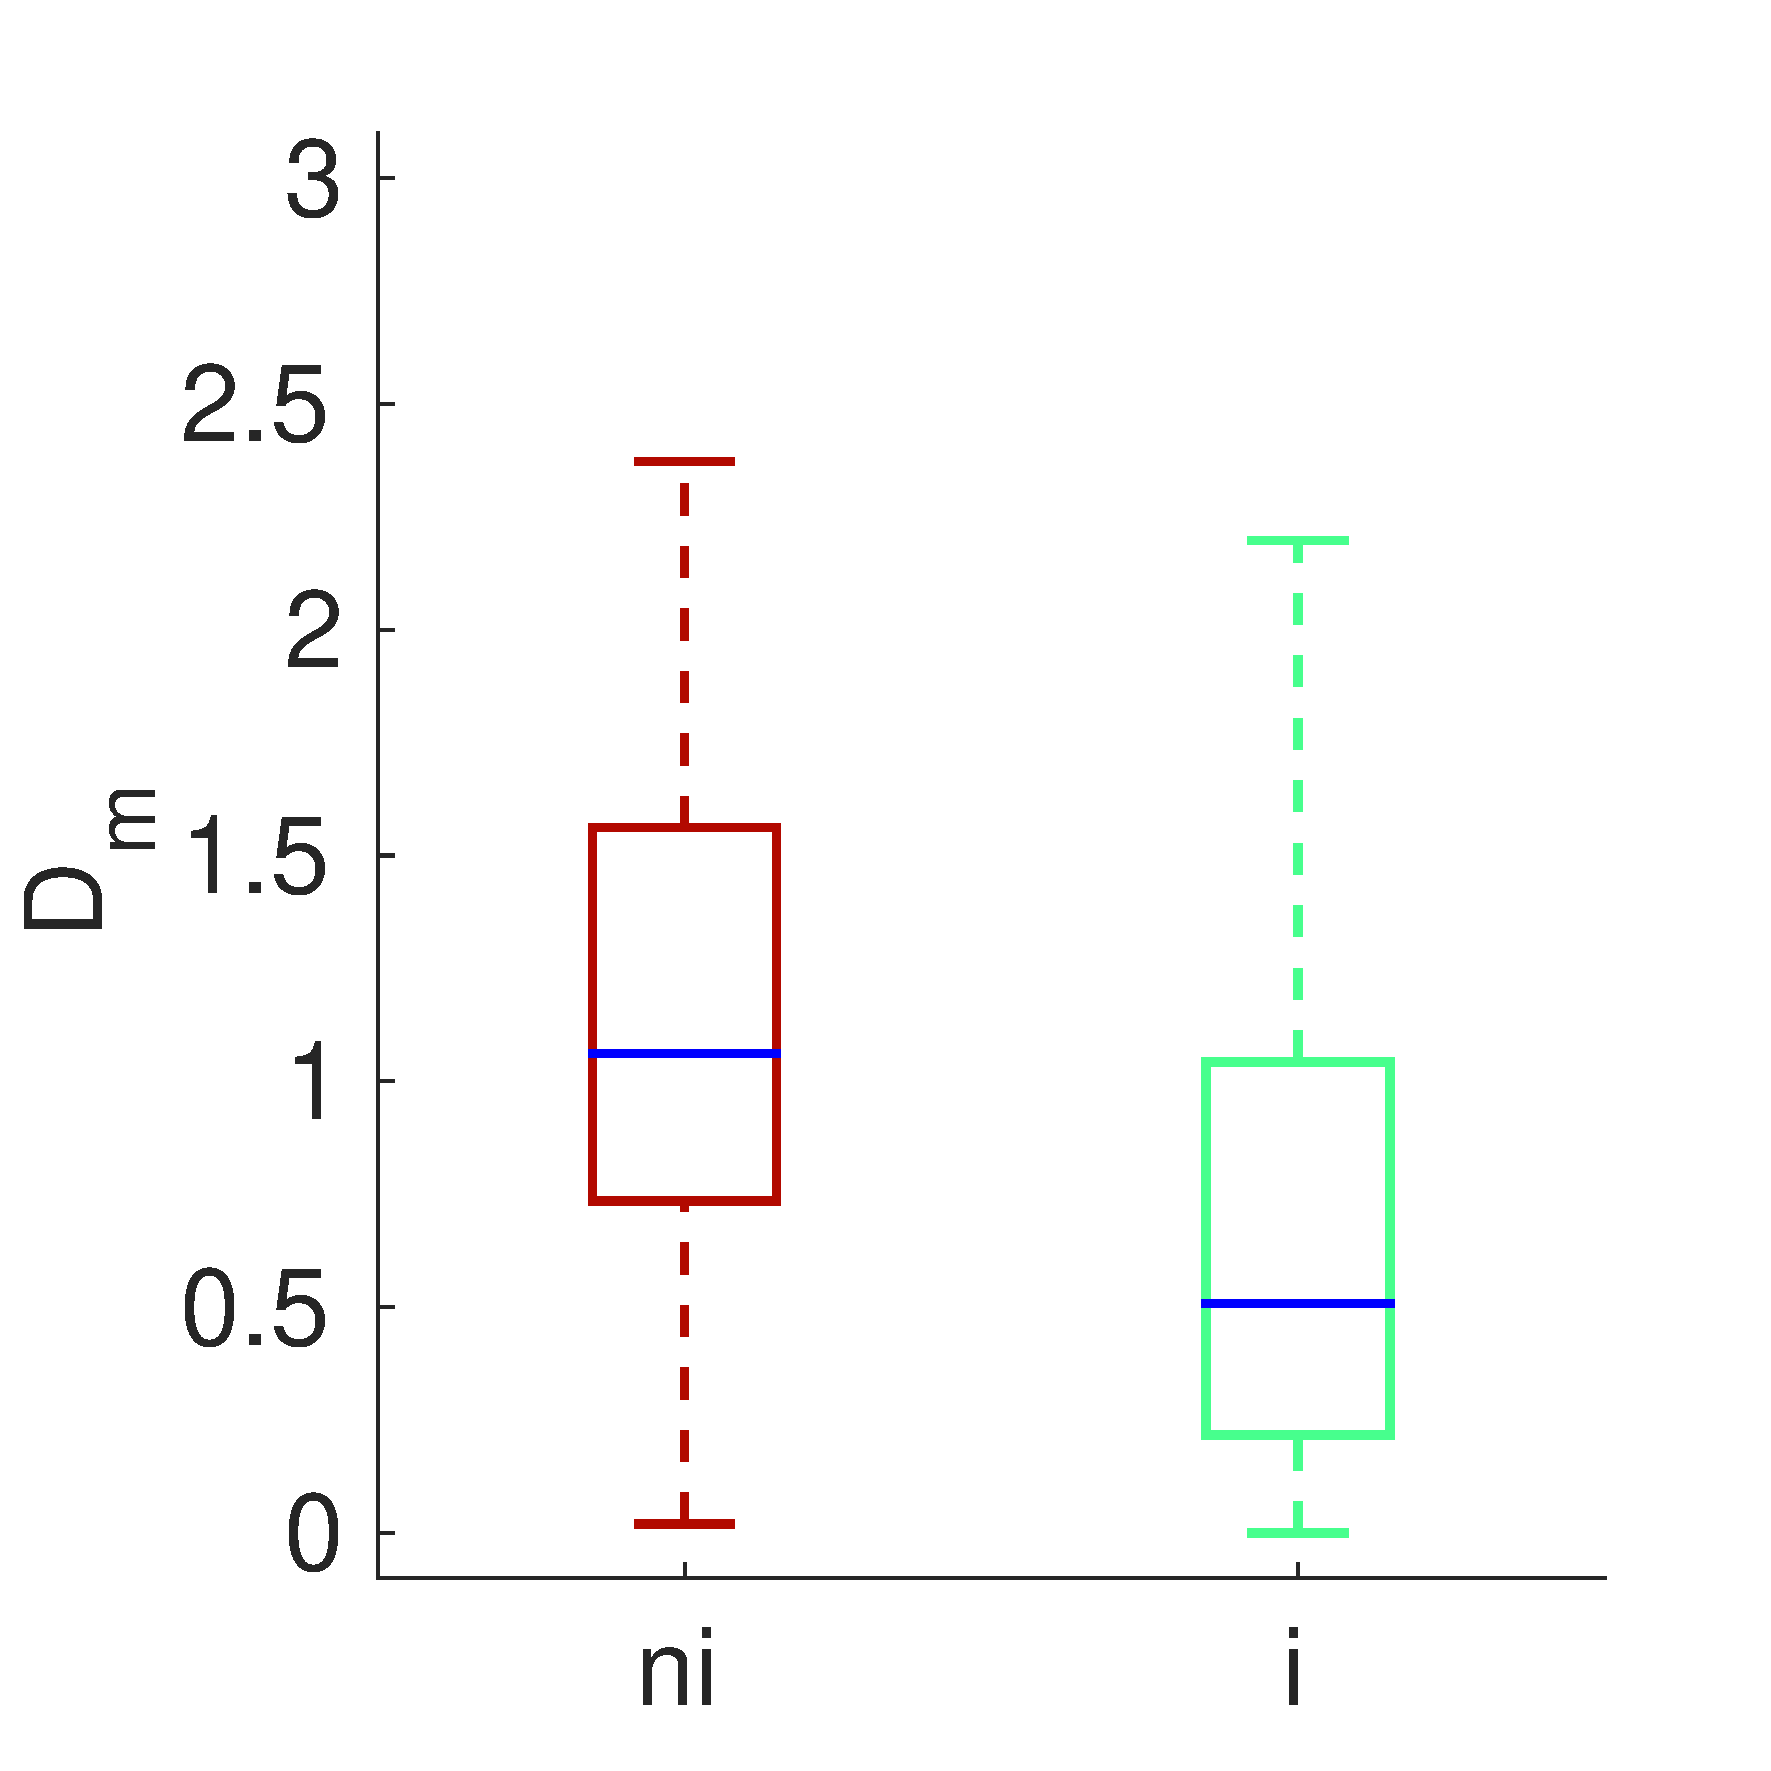
\includegraphics[width=.33\linewidth]{gfxXpUrbanSoundscape/xp_density_7}\label{fig:densityMarkera}}
        \subfloat[]
        {\includegraphics[width=.33\linewidth]{gfxXpUrbanSoundscape/xp_density_9}\label{fig:densityMarkerb}}\par
        \subfloat[]
        {\includegraphics[width=.33\linewidth]{gfxXpUrbanSoundscape/xp_density_8}\label{fig:densityMarkerc}}
        \subfloat[]
        {\includegraphics[width=.33\linewidth]{gfxXpUrbanSoundscape/xp_density_10}\label{fig:densityMarkerd}}
       \caption[TODO]{TODO}\label{fig:densityMarker}
\end{figure}

\begin{figure}[t]
        \myfloatalign
        \subfloat[]
        {\includegraphics[width=.33\linewidth]{gfxXpUrbanSoundscape/xp_soundlevel_7}\label{fig:soundlevelMarkera}}
        \subfloat[]
        {\includegraphics[width=.33\linewidth]{gfxXpUrbanSoundscape/xp_soundlevel_11}\label{fig:soundlevelMarkerb}}
        \subfloat[]
        {\includegraphics[width=.33\linewidth]{gfxXpUrbanSoundscape/xp_soundlevel_15}\label{fig:soundlevelMarkerc}}\par
        \subfloat[]
        {\includegraphics[width=.33\linewidth]{gfxXpUrbanSoundscape/xp_soundlevel_8}\label{fig:soundlevelMarkerd}}
        \subfloat[]
        {\includegraphics[width=.33\linewidth]{gfxXpUrbanSoundscape/xp_soundlevel_12}\label{fig:soundlevelMarkere}}
        \subfloat[]
        {\includegraphics[width=.33\linewidth]{gfxXpUrbanSoundscape/xp_soundlevel_16}\label{fig:soundlevelMarkerf}}\par
        \subfloat[]
        {\includegraphics[width=.33\linewidth]{gfxXpUrbanSoundscape/xp_soundlevel_19}\label{fig:soundlevelMarkerDiffa}}
        \subfloat[]
        {\includegraphics[width=.33\linewidth]{gfxXpUrbanSoundscape/xp_soundlevel_21}\label{fig:soundlevelMarkerDiffb}}
        \subfloat[]
        {\includegraphics[width=.33\linewidth]{gfxXpUrbanSoundscape/xp_soundlevel_23}\label{fig:soundlevelMarkerDiffc}}\par
        \subfloat[]
        {\includegraphics[width=.33\linewidth]{gfxXpUrbanSoundscape/xp_soundlevel_20}\label{fig:soundlevelMarkerDiffd}}
        \subfloat[]
        {\includegraphics[width=.33\linewidth]{gfxXpUrbanSoundscape/xp_soundlevel_22}\label{fig:soundlevelMarkerDiffe}}
        \subfloat[]
        {\includegraphics[width=.33\linewidth]{gfxXpUrbanSoundscape/xp_soundlevel_24}\label{fig:soundlevelMarkerDifff}}
       \caption[TODO]{TODO}\label{fig:soundlevelMarker}
\end{figure}




\subsection{Discussions}

\gl{Résumé des descripteurs utiles}\\
\gl{Pour améliorer une i-scène, on a une triple action: 1) identifier les sons agréables, 2) augmenter le niveau de ces sons et 3) baisser le niveau des autres}\\
\gl{Reprendre la conclusion de l'article}\\
\gl{On a bien montré que les descripteurs à utiliser dépende de la nature de l'environnement. Comme la nature de l'environnement dépend de sa composition, les descripteurs dépendent des sources sonores. Attention cependant, la perception de sources non typique peut elle même varier en fonction du contexte environnemental (\eg~foule)}
\gl{Proposer un modèle perceptive sur la base du modèle prédictif}
\section{Simulation et approche positive}
\label{sec:xp3}

\subsection{Objectif de l'expérience}

\subsection{Planification expérimentale}

\subsection{Données et méthodes d'analyses}

\subsection{Discussions}

\section{Simulation et approche catégorielle}
\label{sec:xp4}

\subsection{Objectif de l'expérience}

\subsection{Planification expérimentale}

\subsection{Données et méthodes d'analyses}

\subsection{Discussions}
%*****************************************
%*****************************************
%*****************************************
%*****************************************
%*****************************************






\cleardoublepage
\ctparttext{preamble text here.}
\part{Analyse automatique des scènes sonores environnementales}
%************************************************
\chapter[État de l'art]{L'analyse automatique des scènes sonores environnementales, un état de l'art}\label{ch:ml_ea}
%************************************************

\gl{annonce de plan}

\section{Introduction}

\subsection{Historique, communauté et application}

\gl{TODO: bioacoustique}
\gl{TODO: introduire AED, ASC et ASSR}

\subsection{Campagnes d'évaluation: le challenge DCASE}
\label{sec:ch6_challengeDcasePresentation}

\gl{TODO: présentation des tâches, des méthodes d'évaluation (chez soi, sur serveur)}

\section{Descripteurs}

\subsection{Spectrogramme}
\label{sec:ch6_spec}

\subsection{Échelle de Bark et de Mel}

\subsubsection{Bark}
\label{sec:ch6_Bark}

\subsubsection{Mel}
\label{sec:ch6_Mel}

\subsection{Coefficients cepstraux}

\subsubsection{Mel-Frequency Cepstral Coefficients}
\label{sec:ch6_mfcc}
\gl{TODO: \citep{Davis80a}}
 
\subsubsection{Gammatone Cepstral Coefficients}
\label{sec:ch6_Gammatone}
 
\subsection{Transformation à Q-constant et Q-variable}
 \label{sec:ch6_VQT_CQT}
 
\subsection{Filtre de Gabor}
\label{sec:ch6_gabor}

\subsection{Scattering}
\label{sec:ch6_scattering}

Scattering transforms are time-shift invariant representations of audio signals consisting of auditory and modulation filter banks interspersed with complex modulus nonlinearities.
This section highlights the importance of invariance to time-shifts and stability to time-warping in the representation of acoustic scenes, and explains how the scattering transform is designed to satisfy these properties while having a high discriminative power.

\subsubsection{Invariance and stability in acoustic scenes}

The notion of invariance to time shifts plays an essential role in acoustic scene similarity retrieval as well as acoustic scene classification.
Indeed, recordings may be shifted locally without affecting their perception and therefore such shifts do not convey any information about the class.
To discard this superfluous source of variability, signals can be mapped to a time-shift invariant feature space before training the classifier, eliminating the need for this classifier to explicitly learn this invariance.
From any time-varying set of descriptors $\boldsymbol{x_1}(t,\gamma)$, where $\gamma$ denotes a descriptor index, a representation invariant to time-shifts shorter in duration than $T$ can be obtained by convolving $\boldsymbol{x_1}$ with a low-pass filter $\boldsymbol{\phi}(t)$ of cutoff frequency set to $1/T$, as measured in Hertz:
\begin{equation}
\mathbf{S_1}\boldsymbol{x}(t, \gamma) = (\boldsymbol{x_1} \ast \boldsymbol{\phi}) (t).
\end{equation}
A downside is that the transient information in $\boldsymbol{x_1}$ at scales finer than $T$ are lost by this low-pass filtering, reducing discriminability in feature space.
To address this issue, the scattering transform recovers this information by convolving $\boldsymbol{x_1}$ with wavelets whose center frequencies are above $1/T$ and then applying complex modulus.

By resorting to wavelet transform modulus, as opposed to Fourier transform modulus, the resulting features are provably stable to time-warping deformation,
in the sense of Lipschitz regularity with respect to diffeomorphisms \cite{Mallat2012}.
In addition to invariance, this stability property is crucial to signal classification, since it guarantees robustness to small variations in pitch, reverberation, and rhythmic organization of events, which make up an important part of the intra-class variability among natural sounds.

Starting from a monophonic waveform $\boldsymbol{x}(t)$, the scattering transform is defined as an infinite cascade of wavelet transform and modulus operators.
However, to achieve invariance to translation up to $T = 372\,\mathrm{ms}$, \ie the approximate minimal duration between non-overlapping acoustic events, two layers of scattering transform often suffice.

The next subsection describes the operations involved in the scattering transform, and in particular the construction of wavelet filter banks.

\subsubsection{Wavelet scalogram}

Our convention for the Fourier transform of a continuous-time signal $\boldsymbol{x}(t)$ is $\boldsymbol{\hat{x}}(\omega) = \int x(t) \exp(\mathrm{i} 2\pi t \omega) \; \mathrm{d}\omega$. Note that the frequency variable $\omega$ is expressed in Hertz, not in radians per second.

Let $\boldsymbol{\psi}(t)$ a complex-valued band-pass filter of
center frequency $\xi_1$ and bandwidth $\xi_1/Q_1$.
A filter bank of wavelets is built by dilating $\boldsymbol{\psi}(t)$
according to a geometric sequence of scales $2^{\gamma_1/Q_1}$, obtaining
\begin{equation}
\boldsymbol{\psi_{\gamma_1}}(t) = 2^{-\gamma_1/Q_1} \boldsymbol{\psi}(2^{-\gamma_1/Q_1} t)\mbox{.}
\end{equation}
The variable $\gamma_1$ is a scale, or an inverse log-frequency, taking integer values between $0$ and $(J_1 \times Q_1 - 1)$.
In the sequel, we set $\xi_1$ to $20~\mathrm{kHz}$ (close to the Nyquist frequency of the audio recordings), the number of octaves $J_1$ to $10$ (the lower end of human hearing range), and the number of wavelets per octave $Q_1$ to $8$.
For each $\gamma_1$, the wavelet $\boldsymbol{\psi_{\gamma_1}}(t)$
has a center frequency of $2^{-\gamma_1/Q_1}\xi_1$, a bandwidth of $2^{-\gamma_1/Q_1}\xi_1/Q_1$, and a quality factor of $Q_1$.

The wavelet transform of an audio signal
$\boldsymbol{x}(t)$ is obtained by convolution with all wavelets.
Applying pointwise complex modulus the transform yields
the wavelet scalogram
\begin{equation}
\boldsymbol{x_1}(t, \gamma_1)
= \vert \boldsymbol{x} \ast \boldsymbol{\psi_{\gamma_1}} \vert (t)\mbox{.}
\end{equation}
The wavelet scalogram bears resemblance to the constant-Q transform (CQT),
which is derived from the short-term Fourier transform (STFT) by averaging the frequency
axis into constant-Q subbands of center frequencies $2^{-\gamma_1/Q_1}\xi_1$.
Indeed, both time-frequency representations are indexed by time $t$ and log-frequency $\gamma_1$.
However, contrary to the CQT, the wavelet scalogram reaches the Heisenberg
theoretical limit of optimal time-frequency localization across the whole
frequency range, whereas the temporal resolution of the traditional CQT is fixed by the support of the STFT analyzing window \cite{Brown1992}.
Therefore, the wavelet scalogram has a better temporal localization at high
frequencies than the CQT, at the expense of a greater computational cost
since the inverse fast Fourier transform (IFFT) routine must be called for each wavelet $\boldsymbol{\psi_{\gamma_1}}$ in the filter bank.
However, this allows us to observe amplitude modulations at fine temporal scales in the scalogram, down to the minimum scale $2Q_1/\xi_1$ for $\gamma_1 = 0$, of the order of $1\,\textrm{ms}$ given the aforementioned values of $Q_1$ and $\xi_1$.

\subsubsection{Extracting modulations with second-order scattering}

Among auditory scenes, amplitude modulations may be caused by a broad variety of mechanical interactions, including collision, friction, and turbulent flow.
At longer scales, they also account for higher-level attributes of sound, such as prosody in speech or rhythm in music.
Although they are discarded while filtering $\boldsymbol{x_1}(t,\gamma_1)$ into a time-shift invariant representation $\mathbf{S_1}\boldsymbol{x}(t,\gamma_1)$, they can be recovered by a second wavelet transform modulus operator.
The amplitude modulation spectrum resulting from this operator is
\begin{equation}
\boldsymbol{x_2}(t,\gamma_1,\gamma_2) =
\vert \boldsymbol{x_1} \ast \boldsymbol{\psi_{\gamma_2}} \vert(t,\gamma_1),
\end{equation}
where the center frequencies of the wavelets $\boldsymbol{\psi_{\gamma_2}}(t)$ are of the form $2^{-\gamma_2/Q_2} \xi_2$, and the second-order scale index $\gamma_2$ takes integer values between $0$ and $(J_2 \times Q_2 - 1)$. Note that these second-order wavelets are dilated versions of a second mother wavelet $\boldsymbol{\psi}$, with a different center frequency $\xi_2$ and quality factor $Q_2$. The identity of the wavelet will be clear from context.
In the sequel, we set $\xi_2$ to $2.5\,\mathrm{kHz}$, $Q_2$ to $1$, and $J_2$ to $12$. Lastly, the low-pass filter $\phi(t)$ is applied to $\boldsymbol{x_2}$ to guarantee invariance to time-shifting, which yields
\begin{equation}
\mathbf{S_2}\boldsymbol{x}(t,\gamma_1,\gamma_2) =
(\boldsymbol{x_2} \ast \phi)(t,\gamma_1,\gamma_2).
\end{equation}
The scattering transform $\mathbf{S}\boldsymbol{x}(t,\gamma)$ consists of the concatenation of first-order coefficients $\mathbf{S_1}\boldsymbol{x}(t,\gamma_1)$ and second-order coefficients $\mathbf{S_1}\boldsymbol{x}(t,\gamma_1,\gamma_2)$ into a feature matrix $\mathbf{S}\boldsymbol{x}(t,\gamma)$, where $\gamma$ is a shorthand for either $\gamma_1$ or $(\gamma_1,\gamma_2)$.

\subsubsection{Gammatone wavelets}
%
%\begin{figure}
%\begin{center}
%\includegraphics[width=\columnwidth]{gammatones}
%\caption{
%\label{fig:gammatones}
%Gammatone wavelets $\psi(t)$ in the time domain with quality factors (a) $Q = 4$ and (b) $Q = 1$. Blue and red oscillations represent the real and imaginary parts. The orange envelope represents the complex modulus.}
%\end{center}
%\end{figure}

Wavelets $\boldsymbol{\psi_{\gamma_1}}(t)$ and $\boldsymbol{\psi_{\gamma_2}}(t)$ are designed as fourth-order Gammatone
wavelets with one vanishing moment \cite{Venkitaraman2014}, and are shown in Figure \ref{fig:gammatones}.
In the context of auditory scene analysis, the asymmetric envelope of Gammatone wavelets is more biologically plausible than the symmetric, Gaussian-like envelope of the more widely used Morlet wavelets.
Indeed, it allows to reproduce two important psychoacoustic effects in the mammalian cochlea: the asymmetry of temporal masking and the asymmetry of spectral masking  \cite{Fastl2007}.
Moreover, it should be noted that Gammatone wavelets follow the typical amplitude profile of natural sounds, beginning with a relatively sharp attack and ending with a slower decay.
As such, they can be discovered automatically by unsupervised encoding of natural sounds \cite{Smith2006}.
This suggests that, despite being hand-crafted and not learned, Gammatone wavelets provide a sparse time-frequency representation of acoustic scenes.

\subsubsection{Logarithmic compression}
\label{sec:ch6_LogComp}

Many algorithms in pattern recognition, including nearest-neighbor classifiers and SVMs, tend to work best when all features follow a standard normal distribution across all training instances \cite{Hsu2003}.
Yet the distribution of the scattering coefficients is skewed towards larger values. We can reduce this skewness by applying a pointwise concave transformation, such as a logarithm, to all coefficients.
Figure \ref{fig:histograms} shows the distribution of an arbitrarily chosen scattering coefficient over the DCASE 2013 dataset, before and after logarithmic compression.

%\begin{figure}
%\begin{center}
%\includegraphics[width=\columnwidth]{compression}
%\caption{
%\label{fig:histograms}
%Histogram of values taken by the first-order scattering coefficient $\mathbf{S}\boldsymbol{x}(\gamma)$, corresponding to a center acoustic frequency of $302\,\mathrm{Hz}$,
%(a) before and (b) after logarithmic compression.}
%\label{fig:compression}
%\end{center}
%\end{figure}


Taking the logarithm of a magnitude spectrum is ubiquitous in audio signal processing.
Indeed, it is corroborated by the Weber-Fechner law in psychoacoustics, which states that the sensation of loudness is roughly proportional to the logarithm of the acoustic pressure. 
We must also recall that the measured amplitude of sound sources often decays polynomially with the distance to the microphone -- a source of spurious variability in scene classification.
Logarithmic compression can linearize this dependency, facilitating the construction of a powerful invariant at the classifier stage.

For the task of musical genre recognition, second-order scattering coefficients $\mathbf{S_2}\boldsymbol{x}(t,\gamma_1,\gamma_2)$ are sometimes normalized by the corresponding first-order scattering coefficients $\mathbf{S_1}\boldsymbol{x}(t,\gamma_1)$, since this decorrelates them from one another \cite{Anden2014}.
We note that taking the logarithm of such renormalized coefficients yields
\begin{equation}
\log \dfrac{\mathbf{S_2}\boldsymbol{x}(t,\gamma_1,\gamma_2)}{\mathbf{S_1}\boldsymbol{x}(t,\gamma_1)} =
\log \mathbf{S_2}\boldsymbol{x}(t, \gamma_1, \gamma_2) -
\log \mathbf{S_1}\boldsymbol{x}(t, \gamma_1),
\end{equation}
\ie a linear combination of the logarithms of first- and second-order coefficients.
As such, a non-linear renormalization becomes a linear transformation, which can be learned by a linearly discriminative classifier.

\section{Algorithmes et classifieurs}

\subsection{Modèle de Markov caché}
\label{sec:ch6_hmm}

\gl{TODO: \citep{Rabiner1989}}

\subsection{Machines à vecteurs de support}
\label{sec:ch6_svm}

\subsection{Factorisation de matrice non-négative}
\label{sec:ch6_nmf}

\subsection{Autres classifieurs}
\label{sec:ch6_autresAlgo}

\gl{TODO: random forest, GMM}

\section{Détection des événements sonores}
\label{sec:ch6_AED}

\subsection{Objectifs}
\label{sec:ch6_objAED}

\gl{TODO: AED}

\subsection{Métrique}
\label{sec:ch6_metriqueAED}

Les performances des algorithme en AED sont évaluées suivant différentes métriques. Deux d'entre elles sont particulièrement utilisées, et notamment dans les challenges DCASE 2013 (\cf~Section~\ref{sec:ch6_dcase2013AED}) et 2016 (\cf~Section~\ref{sec:ch6_dcase2016AED}). Nous les détaillons dans cette section.

La première métrique est la F-mesure \citep{Giannoulis:2013a,Stowell15}, que l'on note $F$ dans ce document. Cette dernière ce calcule comme suit:

\begin{equation}
F=\dfrac{2\times P \times R}{P+R}
\end{equation}

Où $P$ et $R$ représentent respectivement la précision et le rappel. La precision rend compte du rapport entre le nombre d'événements correctement détectés $c$ et le nombre d'événements effectivement détectés par l'algorithme $e$, tandis que le rappel rend lui compte du rapport entre le nombre d'événements correctement détectés $c$ sur le nombre d'événements à détecter $r$ (le nombre d'événements présents dans la scène):

\begin{equation}
P=\dfrac{c}{e}  \quad \textrm{, } \quad R=\dfrac{c}{r} \quad \textrm{, } \quad  e=c+fp \quad \textrm{, } \quad  r=c+fn
\end{equation}

avec $fp$ le nombre de faux positifs, et $fn$ le nombre de faux négatifs.


La deuxième métrique est le taux d'erreur acoustique \citep{poliner2007discriminative,clear}, que l'on note $ER$ dans ce document. Ce dernier ce calcule comme suit:

\begin{equation}
ER=\dfrac{D+I+S}{N}
\end{equation}

avec $N$ le nombre d'événements à détecter \gl{TODO: vérifier}, $D$ le nombre d'événements manqués ($fn$), $I$ le nombre d'événements faussement détectés ($fp$), et $S$ le nombre d'événements substitués, que l'on définit comme $S=min\lbrace D,I\rbrace$.

$F$ et $ER$ peuvent être calculées de deux manières suivant que l'on tienne compte: 

\begin{itemize}
\item du nombre de trames correctement identifiées ($sb$: \emph{segment based});
\item du nombre d'événements correctement identifiées ($eb$: \emph{event based}).
\end{itemize}

Considéré le nombre d'événements plutôt que les trames permets entre autres d'obtenir une mesure de performance indépendante de la durée des événements. Dans ce cas, on considère usuellement qu'un événement est correctement identifié si son \emph{onset} a été correctement identifié, ou si à la fois son \emph{onset} et son \emph{offset} ont été correctement identifiés. La détection d'une frontière (\emph{onset} ou \emph{offset}), est toujours considérée avec un seuil de tolérance.

Ainsi nous notons $F_{sb}$ et $ER_{sb}$, les F-mesures et taux d'erreur acoustiques calculés en tenant compte des trames, et $F_{eb}$ et $ER_{eb}$ les F-mesures et taux d'erreur acoustiques calculés en tenant compte des événements.

La détection de l'offset d'un événement sonore étant est un tâche compliquée, que ce soit pour des algorithmes ou des humains, nous ne considérons dans ce document des mesures de $F_{sb}$ et $ER_{sb}$ calculés en fonction du nombre d'événements dont les \emph{onsets} ont été correctement identifiés.

Enfin, il est possible de calculer ces métriques en 

Ces métriques, si elles sont calculés sans faire de distinction entre les classes, sont susceptible de donner des poids distincts dans l'évaluation entre les classes bien représentées dans la scène, et celles présentant que peu d'événement. Afin de parer à ce biais, il est possible de calculer les métriques séparément pour chaque classe, avant de les moyenner. On note ainsi $Fcw$ et $ERcw$, les versions alternatives de $F$ et $ER$ normalisée par classe:

\begin{equation}
\label{eq:ch7_eq3}
Fcw=\dfrac{1}{C}\sum_{i=1}^C F^i \quad \textrm{, } \quad ERcw=\dfrac{1}{C}\sum_{i=1}^C ER^i
\end{equation}

avec $C$ le nombre de classes à détecter et $F^i$ et $ER^i$, la F-measure et le taux d'erreur acoustique obtenus par un système en ne considérant que la classe d'événements $i$. 

Au final, 8 métriques sont donc disponibles pour évaluer les algorithmes en AED:, nommément $F_{sb}$, $F_{eb}$,$Fcw_{sb}$, $Fcw_{eb}$, $ER_{sb}$, $ER_{eb}$, $ERcw_{sb}$ et $ERcw_{eb}$.

\subsection{Tâche 3 du Challenge \emph{IEEE AASP} DCASE 2013}
\label{sec:ch6_dcase2013AED}

\citep{Giannoulis:2013a,Stowell15}
\gl{TODO: DCASE 2013, fenêtre de tolérance de $\pm100$ms \citep{Giannoulis:2013a,Stowell15} }

\subsection{Tâche 3 du Challenge \emph{IEEE AASP} DCASE 2016}
\label{sec:ch6_dcase2016AED}

\section{Classification des scènes sonores environnementales}
\label{sec:ch6_ASC}

\subsection{Objectifs}
\label{sec:ch6_objASC}

\gl{TODO: ASC}

\subsection{Métrique}
\label{sec:ch6_metriqueASC}

\subsection{Tâche 1 du challenge \emph{IEEE AASP} DCASE 2013}
\label{sec:ch6_dcase2013ASC}

\subsection{Tâche 1 du challenge \emph{IEEE AASP} DCASE 2016}
\label{sec:ch6_dcase2016ASC}

\section{Recouvrement des similarités des scènes sonores environnementales}
\label{sec:ch6_ASSR}

\subsection{Objectifs}
\label{sec:ch6_objASSR}

\gl{TODO: ASSR}

\subsection{Métrique}
\label{sec:ch6_metriqueASSR}

The metric used is the precision at rank $k$ ($p@k$), which is computed by taking a query item and counting the number of items of the same class within the $k$ closest neighbors, and then averaging over all query items. 

\subsection{Méthodes et algorithmes}
\label{sec:ch6_algoASSR}




%*****************************************
%*****************************************
%*****************************************
%*****************************************
%*****************************************





%************************************************
\chapter[Application du modèle à l'évaluation]{Application du modèle morphologique à l'évaluation des algorithmes d'analyse automatique de scènes sonores environnementales}\label{ch:ml_simuperf}
%************************************************

\section{Le challenge DCASE  2013}

\subsection{Objectif}

L'objectif est ici de ré-évaluer les algorithmes soumis dans le cadre de la tâche 2 de détection d'événements sonores (AED) du challenge DCASE 2013 (\cf~Section~\ref{sec:ch6_challengeDcasePresentation}). 

Plus précisément, le but ici est de tester la capacité de généralisation de ces algorithmes, \ie~leur aptitude à maintenir des performances de détection similaires sur plusieurs corpus de scènes présentant des conditions expérimentales différentes.

La généralisation est considérée suivant deux angles:

\begin{itemize}
\item la diversité structurel: évaluer la capacité de généralisation sur des corpus de scènes composés des mêmes samples, mais dont les caractéristiques structurels (intensité sonore des samples, positionnement/espacement moyens des samples) diffèrent;
\item la diversité des samples: évaluer la capacité de généralisation sur des corpus de scènes possédant les mêmes caractéristiques structurels (intensité sonore des samples, positionnement des samples), mais composées d'une sélection de sample différente. Par ``\,sample différent\,'', nous entendons des enregistrement d'événements sonores différents, mais appartenant à la même classe (\eg~claquement de porte). 
\end{itemize}

Le protocole adopté dans ce travail consiste à utiliser le modèle de scènes sonores proposé (\cf~Section~\ref{sec:ch4_modelForm}) afin de générer de nouveaux corpus de scènes simulées, scènes dont nous contrôlons les structures internes, ainsi que la nature des samples utilisés. 

Il s'agit alors d'éprouver les algorithmes sur ces nouveaux corpus, et de comparer leurs performances avec celles obtenus sur le corpus d'évaluation d'origine du challenge DCASE 2013. Les différences nous permettent de conclure quant à la capacité de généralisation des algorithmes considérés.

\subsection{Génération des corpus}

\begin{table}[t]
\begin{center}
\begin{tabular}{lcc}
\textbf{Index} & \textbf{Nom}  & \textbf{Description}  \\ 
\hline
1   & porte-frapper & Frapper à la porte \\
2   & porte-claquer & Claquer la porte \\
3   & parole        & Personne  prononçant \\
    &               &  une phrase \\
4   & rire          & Personne riant  \\    
5   & gorge         & Personne se   \\
    &               & raclant la gorge \\
6   & toux          & Personne toussant \\
7   & tiroir        & Ouverture/fermeture d'un tiroir \\
8   & imprimante    & Bruit d'une imprimante \\
9   & clavier       & Bruit des touches d'un clavier \\
10  & souris        & Bruit d'un clique de souris \\
11  & stylo         & Poser un stylo sur une table \\
12  & bouton        & Bouton permettant d'allumer la lumière \\
13  & clefs         & Poser un jeu de clefs sur une table \\    
14  & téléphone     & Sonnerie de téléphone \\
15  & alerte        & bruit d'une alerte \\
    &               & électronique  (ordinateur, mobile) \\
16  & page          & Tourner une page \\     
\hline      
\end{tabular}
\end{center}
\caption{Classes d'événements sonores utilisées dans le cadre du challenge DCASE 2013}
\label{tab:eventDCASE2013}
\end{table}

Cette section décrit les différents corpus de scènes simulées utilisées lors de l'expérience. 

Tous les corpus  de scènes simulées sont générées à partir des scènes enregistrées du corpus \emph{test-QMUL} : le corpus de \emph{test} de la tâche de détection d'événement (AED) du challenge DCASE 2013  \citep{giannoulis2013detection} (\cf~Section~\ref{sec:ch6_dcase2013AED}). 

\emph{test-QMUL} a été enregistré à l'université \emph{Queen Mary University of London}, il est composé de 11 enregistrements d'ambiances de bureau, toutes d'une durée proche de 1 minute. Chaque scène est une séquence  d'événements sonores non enchevêtrés. Ces événements sont repartis en 16 classes de sons, détaillées dans le tableau~\ref{tab:eventDCASE2013}. Les enregistrements ont été effectués dans 5 environnements acoustiques différents. Les scènes sont annotées par deux individus différents. Pour chaque scène et à chaque événement entendu, l'annotateur indique la classe de l'événement, son \emph{onset} (la position du début de l'événement) et son \emph{offset} (la position de fin de l'événement).  Toutes les annotations sont utilisées, formant ainsi une vérité terrain composée de 22 couples scène-annotateur.


À partir des annotations de \emph{test-QMUL}, quatre corpus de scènes simulées ont été générés, mettant en œuvre deux banques de données de sons isolées ainsi que deux processus de simulation distincts. Les banques de données de sons isolées et les processus de simulation sont détaillés dans les sections suivantes (\cf~Sections~\ref{sec:ch7_eventDataset},~\ref{sec:ch7_simuProcessInstance} et~\ref{sec:ch7_simuProcessAbstract}). 

\begin{figure}[t]
\begin{center}
\includegraphics[width=1\textwidth]{gfx/ch_7/databasesTasslp.pdf}
\label{fig:databasesDCASE2013Simu}
\caption{Generation process of the corpora considered in this evaluation. As part of the DCASE challenge, systems were trained on QMUL Train and tested on QMUL Test during the DCASE challenge.} 
\end{center}
\end{figure}

\subsubsection{Banque de données de sons isolés \emph{QMUL} et \emph{IRCCYN}}
\label{sec:ch7_eventDataset}

Deux banques de sons isolées sont utilisés pour générer les scènes isolées. Elles sont respectivement nommée \emph{QMUL} et \emph{IRCCYN}. Toutes deux sont composés de deux types de sons:

\begin{itemize}
\item les événements: les enregistrements de sons isolés devant être détectés et identifiés par les algorithmes;
\item les \emph{backgrounds}: les enregistrements de fonds sonores, \ie~des scènes amorphes (textures, \cf~Section~\ref{sec:ch4_eventTextureAmorphe}) ne possédant pas d'événement saillant, qui rendent compte de l’environnement acoustique naturel inhérent au lieu d'occurrence des événements. 
\end{itemize}

Les sons isolés de la banque \emph{QMUL} sont extraits de scènes enregistrées à l'université \emph{Queen Mary University of London} (QMUL) dans le cadre de la préparation du challenge AED DCASE-2013, mais n'ayant pas été utilisées lors de l'évaluation,~\ie ne faisant pas partie des corpus de \emph{test} (\emph{test-QMUL}) et de \emph{development}. Ces sons isolées profitent donc des mêmes conditions d’enregistrement que les scènes du corpus \emph{test-QMUL} \citep{Giannoulis:2013a}. Le nombre d'événements par classe varie de 3 à 23. Les enregistrements de \emph{backgrounds} ont été réalisés sur les mêmes environnements acoustiques que ceux utilisés pour le corpus \emph{test-QMUL}, avec là encore les mêmes conditions d'enregistrements.

La banque \emph{IRCCYN} est une nouvelle banque de sons isolés, enregistrées à l'Institut de Recherche en Cybernétique de Nantes (IRCCyN). Cette dernière comprend les mêmes classes que celles présentes dans le corpus \emph{test-QMUL} (\cf~Tableau~\ref{tab:eventDCASE2013}). Les enregistrement ont été effectués dans un environnement calme, à l'aide d'un micro canon \emph{AT8035} connecté à un enregistreur \emph{ZOOM H4n}. Chaque classe est composée de 20 événements sonores, ce qui correspond au nombre d'événements disponibles dans le corpus de \emph{train} du AED DCASE-2013 \citep{Giannoulis:2013a}. Les \emph{background} ont été enregistrés de nuit, dans les bureaux de l'IRCCyN, afin qu'ils ne soient pas pollués par des bruits non souhaités. \\

\gl{TODO: détailler la banque de données IRCCYN}

\subsubsection{Processus de simulation \emph{instance}}
\label{sec:ch7_simuProcessInstance}

Pour le processus de simulation \emph{instance}, l'objectif est de générer des scènes simulées qui ressemblent le plus possible aux scènes du corpus \emph{test-QMUL}. Cette ressemblance se comprend suivant deux aspects:

\begin{itemize}
\item \emph{la structure temporelle}: le positionnement temporel en termes d'\emph{onsets} des événements sonores;
\item \emph{les niveaux sonores des événements}: la puissance du ratio entre l'énergie de l'événement et celle du \emph{background}, notée EBR (\emph{event to Background power Ratios}). L'$EBR$ d'un événement de $N$ échantillons est obtenu en calculant le ratio en décibel entre de la valeur efficace (niveau $RMS$, \cf~Section~\ref{sec:ch5_recordDataSet}) du signal (\cf~Equation~\ref{eq:ch7_eq2}) de l'événement ($E_{rms}$) et du \emph{background}  $B_{rms}$):

\begin{equation}
\label{eq:ch7_eq1}
EBR=20log_{10} \left(  \dfrac{E_{rms}}{B_{rms}} \right) 
\end{equation}

\begin{equation}
\label{eq:ch7_eq2}
X_{rms}=\sqrt{\dfrac{1}{N} \sum_{n=1}^{N} x(n)^2}
\end{equation}

$x(n)$ peut être remplacé par $e(n)$ ou $b(n)$, respectivement les valeurs des signaux de l'événement et du \emph{background} en volt à l'échantillon $n$. 
\end{itemize}

Pour chaque événement et chaque couple scène-annotateur du corpus \emph{test-QMUL}, nous extrayons les positions d'\emph{onsets} et d'{offsets} et calculons une approximation de l'$EBR$. Comme il n'est pas possible d'isoler le signal du \emph{background} des scènes de \emph{test-QMUL}, $B_{rms}$ est obtenu à partir des périodes dénuées d'événements. \\
 
\gl{TODO: expliquer comment on supprime le niveau de bruit dans $E_{rms}$} \\

Les positions \emph{onsets} et les $EBRs$ ainsi recouvrés sont utilisés pour simuler un nouveau corpus de scènes: pour chaque scène simulée, à chaque \emph{onset} d'une annotation (couple scène-annotateur), nous plaçons un événement de la même classe, choisi aléatoirement parmi la banque de sons isolé (\emph{QMUL} ou \emph{IRCCYN}). Afin de garantir que les durées des samples sélectionnés ne soient pas trop long par rapport à celles d'origines, ces derniers sont coupés si leur durée est  supérieure à la durée de l'annotation d'au moins $0.5$ secondes.  Les niveaux des événements des scènes simulées sont fixés par rapports aux $EBRs$ calculés sur les scènes enregistrées. 

Le processus de simulation \emph{instance} ne s'appuie donc pas sur le modèle introduit à la section~\ref{sec:ch4_modelForm}.   L'objectif est d’obtenir des scènes simulées possédant des samples différents des scènes enregistrées, mais dont les structures temporelles et les $EBRs$ sont aussi proches que possible de ceux des scènes du corpus \emph{test-QMUL}.

\subsubsection{Processus de simulation \emph{abstract}}
\label{sec:ch7_simuProcessAbstract}

L'objectif de processus de simulation \emph{abstract} est de capturer les paramètres haut niveaux régissant la structure de la scène enregistrer, et de les utiliser afin de régénérer cette dernière. Le processus \emph{abstract} s'appuie sur le modèle introduit à la section~\ref{sec:ch4_modelForm}. Concrètement, le modèle est instancié suivant des paramètres $\mu_i^a$, $\sigma_i^a$, $\mu_i^t$ et $\sigma_i^t$ (\cf~Équation.~\ref{eq:ch4_eq1} et~\ref{eq:ch4_eq2}) estimés sur la scène enregistrée. Pour chaque couple scène-annotateur du corpus  \emph{test-QMUL}, ces paramètres sont estimés à partir de l'annotation ($\mu_i^t$ et $\sigma_i^t$) et du signal ($\mu_i^a$ et $\sigma_i^a$). Les $EBRs$ et les espacements inter-\emph{onsets} de la scène simulée sont alors obtenus  à partir des distributions normales $\mathcal{N}(\mu_i^a,\sigma_i^a)$ et $\mathcal{N}(\mu_i^t,\sigma_i^t)$ respectivement. Pour chaque classe, le début et la fin des pistes des scènes simulées sont les mêmes que ceux des scènes enregistrées.

Comme pour le processus de simulation \emph{instance}, les événements sont choisis aléatoirement. Afin de garantir que les durées des événements des scènes simulées ne soient pas trop long par rapport à ceux des scènes enregistrées, la durée $D$ d'un sample d'une classe $i$ est seuillé si:

\begin{equation}
D-\mu_i^d-\sigma_i^d>5
\end{equation}

avec, $\mu_i^d$ et $\sigma_i^d$ les moyennes et écart type des durées des samples appartenant à la classe $i$ pour une annotation donnée. La limite de 5 secondes permet de minimiser l'impact d'une telle opération de seuillage sur les sons impulsifs.

\subsubsection{Banque de données de scènes simulées}
\label{sec:ch7_datasetEtEbr}

Cinq corpus sont considérés pour l'évaluation (\cf~Figure~ref{fig:databasesDCASE2013Simu}), à savoir, le corpus de scènes enregistrées \emph{test-QMUL}, et quatre corpus de scènes simulées:

\begin{itemize}
\item \emph{instance-QMUL} (insQ);
\item \emph{abstrait-QMUL} (absQ);
\item \emph{instance-IRCCYN} (insI);
\item \emph{abstrait-IRCCYN} (absI).
\end{itemize}

Les labels ``\,QMUL\,'' et ``\,IRCCYN\,'' font références aux banques de données de sons isolées utilisées pour générer les scènes simulées. Les labels ``\,instance\,'' et ``\,abstract\,'' désignent eux les processus de simulation utilisés. 

Afin d'évaluer l'influence du niveau relatif des événements par rapport au \emph{background} sur les performances des algorithmes, le corpus \emph{instance-QMUL} est composé de quatre sous-corpus appelés respectivement \emph{insQ-EBR(6)}, \emph{insQ-EBR(0)}, \emph{insQ-EBR(-6)} et \emph{insQ-EBR(-12)}. Pour \emph{insQ-EBR(0)}, les $EBRs$ estimés sur \emph{test-QMUL} sont préservés.  Pour \emph{insQ-EBR(6)}, \emph{insQ-EBR(-6)} et \emph{insQ-EBR(-12)}, des compensations de +6$dB$, -6$dB$, -12$dB$ sont ajoutés lors de la simulation aux $EBRs$ d'origines. A noter que pour ces sous-corpus, seul l'$EBR$ est modifié, les positions temporels des événements ainsi que les samples sélectionnés sont strictement identiques entre les quatre sous-corpus.

Pour tous les corpus (\emph{abstract-QMUL}, \emph{instance-IRCCYN} et \emph{abstract-IRCCYN}), ainsi que les sous-corpus de \emph{instance-QMUL}, une simulation est réalisé pour chaque couple scène-annotateur de \emph{test-QMUL} ($11\times2=22$ couples). 

De plus, chaque simulation est répliquée 10 fois. A chaque réplication, la sélection aléatoire des samples varie. Pour les corpus générés suivant le processus de simulation \emph{abstract} (\emph{abstract-QMUL} et \emph{abstract-IRCCYN}), les $EBRs$ et espacements inter-\emph{onsets} des samples obtenus à partir des distributions normales  $\mathcal{N}(\mu_i^a,\sigma_i^a)$ et $\mathcal{N}(\mu_i^t,\sigma_i^t)$ sont également re-tirés d'une réplication à une autre \gl{TODO: A vérifier}. Chaque corpus/sous-corpus est ainsi composé de 220 scènes simulées ($11\times2\times10$).

Tous les corpus sont disponibles en ligne\footnote{Dataset URLs: \begin{itemize}
\item \emph{test-QMUL}: \url{https://archive.org/details/dcase2013_event_detection_testset_OL};
\item \emph{instance-QMUL}, \emph{abstract-QMUL}: \url{https://archive.org/details/dcase_replicate_qmul};
\item \emph{instance-IRCCYN}, \emph{abstract-IRCCYN}: \url{https://archive.org/details/dcase_replicate.
irccyn}
\end{itemize}} et ont été simulée à l'aide de l'outil de simulation MATLAB développé dans le cadre de cette thèse (\cf~Section~\ref{sec:ch4_modAnaAuto}).

\subsubsection{Analyse du réalisme des scènes simulées}

Afin d'évaluer le réalisme des scènes acoustiques simulées, une expérience sensorielle d'analyse sémantique différentielle est conduite. \\

\textbf{Procédure} \\

22 stimuli doivent être noté, comprenant 11 scènes enregistrés de \emph{test-QMUL} et 11 scènes simulées de \emph{instance-IRCCYN}. Les sujets doivent évaluer le réalisme de chaque scène suivant une échelle graduée de 7 points allant de 1 (non réaliste) à 7 (très réaliste). 

L'ordre de présentation est différent pour chaque sujet. Les sujets doivent écouter la totalité d'une scène avant de se prononcer.

À la fin de l'expérience, les sujets sont invités à commenter librement leurs notations. \\

\textbf{Apparatus} \\

L'audio est diffusé en monophonique. Au début de l'expérience, il est demandé aux sujets d'utiliser un casque audio, et de régler le volume sonore à un niveau confortable.  \\

\textbf{Participant} \\

15 sujets ont participé à l'étude. Tous ont réalisé l'expérience avec succès. \\

\textbf{Résultats} \\

Nous considérons $\mathcal{R}_{sujet}$ les notes de réalisme par sujet, moyennée en considérant séparément les scènes de \emph{test-QMUL} et celles de \emph{instance-IRCCYN}.

Les $\mathcal{R}_{sujet}$ les scènes enregistrées et celles simulées sont respectivement de $4.4$ et $3.3$ (\cf~Figure~\ref{fig:xpRealism}), et présente une différence significative (t-test appariées: $p<0.01$). D'après les commentaires des sujets, il semble que les scènes enregistrées n'ait pas été perçues comme très réaliste à cause de leur caractère scriptée, les sujets ayant reconnu le fait qu'il s'agit de scènes jouées. 

En ce qui concerne les scènes simulées, les sujets ont rapporté que: 

\begin{itemize}
\item ``\,le fond sonore semble synthétique/artificiel\,'',  bien que ce dernier ait été enregistré;
\item ``\,certains événements sont coupés\,''. Ce dernier point est en effet avéré. La coupe de certains événements est due à un choix de conception du corpus \emph{instance-IRCCYN} discuté à la section~\ref{sec:ch7_simuProcessInstance}. Ce choix est pris dans le but de minimiser la différence entre la scène simulée et celle de référence. 
\end{itemize}

Il convient de noter que, pour de nombreux participants, certaines scènes simulées ont reçu une note de réalisme plus élevée que certaines des scènes naturelles, ce qui montre que, bien que des différences notables peuvent être faites, ils n'influencent pas le réalisme acoustique par une grande marge.

\begin{figure}[t]
\begin{center}
\includegraphics[width=.33\textwidth]{gfx/ch_7/xp_realism_2}
\caption{Distribution des notes de réalisme $\mathcal{R}_{sujet}$ pour les scènes enregistrés \emph{test-QMUL} et les scènes simulées \emph{instance-IRCCYN}}
\label{fig:xpRealism} 
\end{center}
\end{figure}

\subsection{Métrique}

La métrique considérée dans cette analyse est $Fcw_{eb}$ (\cf~Section~\ref{sec:ch6_metriqueAED}), \ie~la moyenne  des F-mesures calculées séparément pour chaque classe, en tenant compte des \emph{onsets} des événements et avec une fenêtre de tolérance de 100 ms. Cette dernière a l'avantage: 

\begin{itemize}
\item d'être  facilement interprétable;
\item de ne favoriser aucune classe.
\end{itemize}

\subsection{Données et analyses}

\gl{TODO: deux analyse séparé QMUL et IRCCYN, moyenne par réplication et par sample, et paired ttest}

\subsection{Système de détection}

\begin{figure}
\center
\tikzset{mynode/.style={rectangle,rounded corners,draw=black, top color=white, text centered},} 
\tikz \draw [o->] (0,0) -- (1\textwidth,0)
node[mynode, pos=0.15] {\footnotesize Pre-traitement$*$} 
node[mynode, pos=0.38]  {\footnotesize Descripteurs}
node[mynode, pos=0.6]  {\footnotesize Classifieurs} 
node[mynode, pos=0.85] {\footnotesize Post-traitement$*$} 
node[pos=0.15, below=10pt] {\footnotesize dé-bruitage} 
node[pos=0.38, below=10pt] {\footnotesize MFCCs} 
node[pos=0.6, below=10pt] {\footnotesize HMM} 
node[pos=0.85, below=10pt] {\footnotesize lissage};
\caption[Vision schématisée des systèmes de détection d'événements du challenge DCASE 2013]{Vision schématisée des systèmes de détection d'événements du challenge DCASE 2013; $*$ indique que le nœud n'est pas systématiquement utilisé; les choix états de l'art sont données en exemples sous les nœuds.}
\label{fig:schematicSys}
\end{figure}

\begin{table}[t]
\begin{center}
\tiny
\begin{tabular}{lcccc}
\textbf{Système}                    & \textbf{Descripteur} & \textbf{Classifieur}         & \multicolumn{2}{c}{Gestion du bruit}  \\ 
                                    &                      &                              & réduction & apprentissage  \\ 
\hline
CPS                                 & fusion               & Seuil \hfill (D)             &           &             \\ 
\citep{CPS}                         &                      & rapport de vraisemblance \hfill (C)  &           &             \\ 
\hline         
DHV                                 & MFCC                 & HMM \hfill  (D, C)           &           &              \\ 
\citep{diment2013sound,DHV}         &                      &                              &           &             \\ 
\hline 
GVV                                 & mel                  & NMF \hfill  (D, C)           &           &              \\
\citep{gemmeke2013exemplar,GVV}     &                      & HMM \hfill  (P)              &           &             \\                      
\hline
NR                                  & MFCC                 & SVM \hfill   (C)             &           &             \\
\citep{roma2013recurrence,NR2}      &                      &                              & x         &             \\    
\hline
NVM                                 & fusion               & HMM hiérarchique \hfill  (C) &           &            \\     
\citep{niessen2013hierarchical,NVM} &                      & RF  \hfill (C)               &           &            \\     
\hline
SCS                                 & GF                   & HMM \hfill  (C)              & x         &               \\  
\citep{schroder2013use,SCS}         &                      &                              &           &             \\    
\hline  
VVK                                 & MFCC                 & GMM \hfill  (D, C)           &           & x            \\ 
\citep{VVK,gemmeke2013exemplar}     &                      &                              &           &             \\    
\hline
Baseline                            & CQT                  & NMF \hfill  (D, C)           &           &             \\ 
\citep{Giannoulis:2013a}            &                      &                              &           &             \\  
\hline      
\end{tabular}
\end{center}
\caption[Description synthétique des systèmes soumis dans le cadre de la tâche 2 de challenge DCASE 2013]{Description synthétique des systèmes soumis dans le cadre de la tâche 2 de challenge DCASE 2013; (D) indique une étape de détection, (C) de classification et (P) de post-traitement}
\label{tab:systemsDcase2013}
\end{table}

Tous les algorithmes ayant été évalués lors de la tâche 2 (AED) du challenge DCASE 2013 sont considérés dans cette étude (\cf~Tableau~\ref{tab:systemsDcase2013}). Un total de 8 algorithmes ont été soumis, auxquels nous rajoutons la \emph{baseline} fournie par les organisateurs du challenge.

La majorité des systèmes suivent la chaîne de traitement illustrée à la figure~\ref{fig:schematicSys}, incluant parfois une étape de prétraitement de dé-bruitage.

Le classifieur de choix est un HMM (\cf~Section~\ref{sec:ch6_hmm})  à 2 couches, où la première modélise l'événement et la seconde la transition entre les événements. D'autres classifieurs incluant les forêts d'arbres décisionnels (RF: \emph{Random Forests}, \cf~Section~\ref{sec:ch6_autresAlgo}), les machines à vecteurs de support (SVM: \emph{Support Vector Machines}, \cf~Section~\ref{sec:ch6_svm}) la factorisation de matrice non-négative (NMF: \emph{Non-negative Matrix Factorization}, \cf~Section~\ref{sec:ch6_nmf}), ainsi que des modèle de mélanges gaussiens (GMM: \emph{Gaussian mixture model}, \cf~Section~\ref{sec:ch6_autresAlgo}) sont également utilisés. Nous invitons le lecteur à se référer à \citep{Stowell15} ou/et aux publications indiquées dans le tableau~\ref{tab:systemsDcase2013} pour une description détaillée des algorithmes.


Au niveau des descripteurs on distingue 5 groupes:

\begin{itemize}
\item \emph{mel}: une représentation temps-fréquence où l'axe fréquentiel à été projeté sur une échelle de Mel. Nous invitons le lecteur à se référer à la section~\ref{sec:ch6_Mel} pour une description synthétique de l'échelle de mel;
\item \emph{CQT}: une représentation temps-fréquence calculée en \gl{TODO}. Nous invitons le lecteur à se référer à la section~\ref{sec:ch6_VQT_CQT} pour une description de la CQT;
\item \emph{MFCC}: une représentation basée sur des coefficients cepstraux calculées sur échelle de Mel (MFCCs: \emph{Mel-Frequency Cepstral Coefficients}). Nous invitons le lecteur à se référer à la section~\ref{sec:ch6_mfcc} pour une description des MFCCs;
\item \emph{GF}: une représentation temps-fréquence filtrée par un banc de filtres de Gabor (GF: \emph{Gabor filterbank}). Nous invitons le lecteur à se référer à la section~\ref{sec:ch6_gabor} pour une description des filtres de Gabor;
\item \emph{fusion}: les algorithmes utilisant simultanément plusieurs descripteurs. NVM et CPS utilisent des jeux de descripteurs allant d'indicateurs scalaires rendant compte des caractéristiques temporelles (\eg~\emph{flatness}) et fréquentielles (\eg~\emph{loundness}, centroïde spectral) du signal, à des descripteurs multidimensionnelles (\eg~bandes Mel, MFCC).
\end{itemize}

Tous les algorithmes sont entraînés et paramétrés sur les corpus de \emph{train} et de \emph{development} fournis par les organisateurs du challenge DCASE 2013. \\

\subsection{Résultats}

\subsubsection{Corpus QMUL}

\begin{table} 
\begin{center}  
\begin{tabular}{lccc}  
Système  & testQ & insQ-EBR(0) & absQ \\ 
\hline 
Baseline & \textbf{ 9.0$\pm$4.8}     & \textbf{10.5$\pm$3.0$^*$}   & \textbf{ 9.9$\pm$3.5} \\ 
CPS      & \textbf{0.7$\pm$0.8}      & \textbf{0.8$\pm$1.3}        & \textbf{0.8$\pm$1.4$^*$} \\ 
DHV      & \textbf{30.7$\pm$8.4}     & \textbf{34.5$\pm$7.5$^*$}   & \textbf{34.0$\pm$7.9} \\ 
GVV      & \textbf{13.2$\pm$8.0}     & \textbf{15.0$\pm$6.4$^*$}   & \textbf{14.6$\pm$6.2} \\ 
NR       & \textbf{21.5$\pm$6.5$^*$} &  6.8$\pm$5.7                &  7.4$\pm$5.8 \\ 
NVM      & \textbf{28.2$\pm$5.9$^*$} &  9.7$\pm$9.6                & 10.8$\pm$9.9 \\ 
SCS      & \textbf{41.5$\pm$7.6$^*$} & \textbf{39.3$\pm$8.2}       & \textbf{39.4$\pm$8.2} \\ 
VVK      & \textbf{24.6$\pm$6.8$^*$} & \textbf{19.7$\pm$8.7}       & \textbf{19.2$\pm$9.2} \\  
\hline
\end{tabular} 
\end{center} 
\caption[Résultats en considérant $Fcw_{eb}$ pour chacun des systèmes évalués et chaque corpus considéré dans le cadre du challenge DCASE 2013]{Résultats en considérant $Fcw_{eb}$ pour chacun des systèmes évalués et chaque corpus considéré dans le cadre du challenge DCASE 2013. Les résultats en gras ne présentent pas de différence significative (t-test à deux populations appariées) avec le meilleur résultat de la ligne (indiqué par $^*$).} 
\label{tab:qmul} 
\end{table} 

\begin{table}
\begin{center} 
\begin{tabular}{lllllll}  
  Système &   testQ         &  insQ-EBR(0)      &   absQ          \\
 \hline
 Baseline & 3.14            &  8.63             &  7.40    \\
          & (tiroir)        &  (tiroir)         & (tiroir) \\
      CPS & 2.66            &  9.04             &  7.84   \\
          & (porte-frapper) & (porte-claquer)   & (porte-claquer) \\
      DHV & 8.44            &  6.88             &  8.01  \\
          & (tiroir)        &  (tiroir)         &  (clavier)  \\
      GVV & 3.08            &  3.78             &  3.55   \\
          & (page)          &  (page)           & (page) \\
      NR  & 4.33            & \textbf{25.35}    & \textbf{20.68}  \\
          & (clavier)       & (porte-claquer)   & (porte-claquer)  \\
      NVM & 1.26            & \textbf{22.48}    & \textbf{19.22}    \\
          & (rire)          & (toux)            & (toux) \\
      SCS & 1.18            &  2.70             &  1.72   \\
          & (alerte)        &  (tiroir)         & (porte-claquer)  \\
      VVK & 1.81            &  8.73             &  8.20   \\ 
          & (alerte)        &  (porte-claquer)  & (porte-claquer) \\
       \hline
\end{tabular}
\end{center} 
\caption[Nombre maximum de faux positifs pour chaque système évalué et pour chaque corpus]{Nombre maximum de faux positifs pour chaque système évalué et pour chaque corpus. Les résultats sont moyennés suivant les enregistrements. Les classes de sons correspondantes sont indiquées entre parenthèse.}
\label{tab:fp}
\end{table}

Avec la permission des auteurs des différents systèmes proposés (\cf~Tableau~\ref{tab:systemsDcase2013}), ces derniers sont testés sur les corpus de scènes simulées, en utilisant les mêmes serveurs de calculs que ceux utilisés pour la tache 2 (AED) du challenge DCASE 2013. Les systèmes ont par ailleurs été re-testés sur le corpus \emph{test-QMUL} (corpus de \emph{test} du challenge AED DCASE 2013), afin de vérifier la réplicabilité des résultats précédemment publiés \citep{Stowell15}.

Le Tableau~\ref{tab:qmul} affiche les $f_c$ en pourcentage pour les corpus \emph{test-QMUL}, \emph{insQ-EBR(0)} et \emph{abstract-QMUL}. Les performances pour \emph{baseline}, CPS, DHV, GVV, SCS et VVK ne présentent pas de différences significatives entre les trois corpus. Les résultats de NVM et NR décroissent significativement entre \emph{test-QMUL} et les deux corpus \emph{insQ-EBR(0)} et abstract-QMUL ($p<0.01$).

Le système CPS, tel que soumis au challenge DCASE 2013, présente un problème d'implémentation l'empêchant de fonctionner correctement. Ce problème est à l'origine des faibles résultats obtenus pour \emph{test-QMUL}, résultats qui se retrouvent sur \emph{insQ-EBR(0)} et \emph{abstract-QMUL}. Pour ces raisons nous ne considérons pas plus avant ce système.

Exception faite de NR et NVM, les classements des systèmes établis par rapport à leur performances sont égaux pour les 3 corpus. Ces résultats permettent de conclure deux points quant aux performances de DHV, GVV, SCS et VVK:

\begin{itemize}
\item comparaison entre \emph{test-QMUL} et \emph{insQ-EBR(0)}: les performances comparables montrent que les algorithmes sont robustes au changement d'événements. À noter que les samples proviennent tous des enregistrements de QMUL, \ie~ont été enregistrés dans les mêmes conditions;
\item comparaison entre \emph{test-QMUL} et \emph{abstract-QMUL}: les performances comparables montrent que les algorithmes sont robustes à un changement de positions temporels des samples, si les paramètres structuraux des scènes ($EBRs$ et espacement inter-\emph{onsets}) sont conservés.
\end{itemize}
  
Nous examinons maintenant les raisons pouvant expliquer les chutent de performances des systèmes NVM et NR dans le cas des scènes simulées. En effet, la chute peut être due soit à l'incapacité des algorithmes à généraliser sur d'autres corpus, soit à un artefact produit par les processus de simulation.

Pour les deux algorithmes, la première étape du traitement consiste à extraire des descripteurs sur l'ensemble des trames du signal, et la deuxième à classifier les trames.

Considérons dans un premier temps les descripteurs extraits. Les valeurs minimales et maximales ne varient pas entre \emph{test-QMUL} et les corpus de scènes simulées. Les distributions des valeurs des descripteurs entre les deux types de corpus présentent certes une différence, mais cette dernière se révèle faible et non-significative. \gl{TODO: test ?} 

Une inspection des matrices de confusion inter-classes révèle que c'est, pour les deux systèmes, l'étape de classification qui serait responsable de la dégradation des performances. Le tableau~\ref{tab:fp} affiche, pour tous les systèmes, le plus grand nombre de faux positifs moyenné sur l'ensemble des scènes pour les trois corpus, ainsi que la classe correspondante. Pour NVM et NR, une classe en particulier (NVM: toux, NR: porte-claquer) semble être détectée de manière abusive, augmentant drastiquement le nombre de faux positifs, et diminuant \emph{de facto} les résultats.

Nous concluons que, pour ces deux systèmes, la diminution des performances n'est probablement pas un artefact dû au processus de simulation, mais plutôt a un phénomène de sur-apprentissage de l'étape de classification. Considérant que ces systèmes sont les seuls à faire usage d'une approche de classification discriminative (NR: SVMs; NVM: RFs), nous conjecturons que le cadre d'entraînement proposé par le challenge DCASE, et notamment le faible nombre de samples disponible pour l'apprentissage (20 par classe) \gl{TODO: A vérifier}, n'est pas adapté pour ces deux algorithmes.

Nous considérons maintenant l'influence de l'$EBR$ sur les performances des algorithmes. Les résultats obtenus pour les corpus \emph{insQ-EBR(-12)}, \emph{insQ-EBR(-6)}, \emph{insQ-EBR(0)} et \emph{insQ-EBR(6)} (\cf~Section~\ref{sec:ch7_datasetEtEbr}) sont présentés sur la figure~\ref{fig:ebr}. 

Sans surprise, plus l'$EBR$ est faible, et plus les performances diminuent. Par ailleurs, plus l'$EBR$ est faible, et plus les  écarts entre les algorithmes se réduisent. Tous les algorithmes, excepté DHV et SCS, ont des performances similaires ou moindres comparées à celle de la \emph{baseline}. L'influence de l'$EBR$ est cohérent, le classement entre en termes de performances entre les algorithmes étant maintenu pour les différents corpus. \gl{TODO: expliquer pourquoi la baseline ne varie pas}

Le seul système qui ne suit pas cette tendance est SCS, qui maintient des performances stables pour les différents $EBRs$. Les performances augmentent entre les $EBRs$ allant de 6 à -6$dB$. Ces résultats sont dus au fait que SCS bénéficie d'une  étape de dé-bruitage, pré-traitement qui est au cœur de l'algorithme de SCS \citep{SCS}.

L'ensemble de ces résultats montrent l'utilité des processus de simulation proposées (\cf~Sections~\ref{sec:ch7_simuProcessAbstract} et~\ref{sec:ch7_simuProcessInstance}), ces derniers permettant bien de répliquer ou d'aller plus loin dans l'analyse des performances des algorithmes.

\begin{figure}[t]
\begin{center}
\includegraphics[width=1\textwidth]{gfx/ch_7/ebr}
\caption{Class wise event based F-measure (in percent) achieved by the systems on the QMUL instance datasets with varying EBR.}
\label{fig:ebr} 
\end{center}
\end{figure}

\subsubsection{Corpus IRCCYN}

\begin{table}
\begin{center} 
\begin{tabular}{lccc}
système  & testQ & insI & absI \\ 
\hline 
Baseline & \textbf{9.0$\pm$4.8$^*$}  &  5.9$\pm$2.9 &  5.6$\pm$2.9 \\ 
DHV      & \textbf{30.7$\pm$8.4$^*$} & 10.0$\pm$5.8 &  9.5$\pm$5.6 \\ 
GVV      & \textbf{13.2$\pm$8.0$^*$} &  5.6$\pm$3.7 &  5.5$\pm$3.6 \\
NR       & \textbf{21.5$\pm$6.5$^*$} &  4.6$\pm$3.4 &  5.4$\pm$4.5 \\ 
NVM      & \textbf{28.2$\pm$5.9$^*$} &  3.1$\pm$3.1 &  3.2$\pm$3.0 \\ 
SCS      & \textbf{41.5$\pm$7.6$^*$} & 35.4$\pm$7.2 & 34.0$\pm$6.7 \\ 
VVK      & \textbf{24.6$\pm$6.8$^*$} &  6.6$\pm$5.7 &  7.3$\pm$6.3 \\ 
\hline
\end{tabular} 
\end{center}  
\caption{Results of the evaluated systems on the IRCCYN datasets, compared with the \emph{test-QMUL} dataset. Results in bold are equivalent (t-test per row at 0.05 significance level) to the best performance (depicted with a $^*$).}
\label{tab:irccyn} 
\end{table} 

Quand on considère une tâche de classification, un problème de taille est de savoir si le système évalué est capable de généraliser ses capacités de classification à des données non-observées, mais qui correspondent aux classes considérées dans les corpus de \emph{train} et de \emph{development}.

Afin d'évaluer les capacités de généralisation des algorithmes, nous considérons les performances obtenus sur les corpus de scènes simulées avec la banque de donnée de sons isolés \emph{IRCCYN}, à savoir \emph{abstract-IRCCYN} et \emph{instance-IRCCYN}, dont les samples (événements et \emph{background}) ont été enregistrés dans des environnements acoustiques différents de ceux des corpus \emph{test-},  \emph{abstract-} et \emph{instance-QMUL}.

Les résultats sont affichés sur le tableau~\ref{tab:irccyn} et la figure~\ref{fig:irccyn}. Alors que la plupart des systèmes ont obtenus des performances comparables entre \emph{test-QMUL} et les corpus \emph{abstract-} et \emph{instance-QMUL}, tous algorithmes voient leurs résultats diminuer de manière significative pour les corpus  \emph{abstract-} et \emph{instance-IRCCYN}. De plus, à l'exception du système SCS, tous les systèmes ont des résultats équivalents à la \emph{baseline} pour les corpus \emph{IRCCYN}, en particulier le système DHV, qui pourtant montre de bons résultats pour les corpus \emph{QMUL}.

L'ensemble de ces résultats nous permettent de conclure que, pour les systèmes DHV, GVV, NR, NVM et VVK, le gain de performance par rapport à la baseline observé sur le corpus \emph{test-QMUL} n'est dû qu'à une sur-adaptation des systèmes aux données d'entraînement (corpus \emph{train}). 

Comme on peut clairement le voir sur la figure~\ref{fig:irccyn}, seul le système SCS (gagnant du challenge AED DCASE 2013), arrive à maintenir des performances similaires entre tous les corpus considérés. Cette capacité de généralisation est par ailleurs cohérente, le système parvenant en effet à généraliser sur des scènes dont on a fait varier: 

\begin{itemize}
\item les samples sélectionnés (en considérant deux banques de sons isolés différents);
\item les positions temporels des samples;
\item les $EBRs$.
\end{itemize}

\begin{figure}[t]
\includegraphics[width=1\textwidth]{gfx/ch_7/irccyn}
\caption{Performances des systèmes évaluées dans le cadre du challenge DCASE 2013 sur les corpus QMUL et IRCCYN en considérant $Fcw_{eb}$.}
\label{fig:irccyn}
\end{figure}

\subsection{Discussion}


Pour résumer les résultats présentés précédemment, l'utilisation des scènes simulées à partir du modèle de scènes sonores proposé nous a permis de:

\begin{enumerate}
\item reproduire le classement des systèmes dans les mêmes conditions d'enregistrement pour les 5 d'entre eux. Les deux systèmes posant problèmes (NR et NVM) présentent des performances dégradées. Nous montrons que cette dégradation est probablement due à un sur apprentissage de leurs  classifieurs discriminants respectifs;
\item évaluer les capacités de généralisation des systèmes dans de nouvelles conditions d'enregistrement. A cet égard, le système SCS est le seul à généraliser correctement;
\item évaluer la robustesse des systèmes lorsque devant traiter des niveaux de bruits de fond différents. Une nouvelle fois, le système SCS est le seul a présenter des performances stables pour les différents $EBR$ considérés, et ce probablement en raison d'une étape efficace de pré-traitement du bruit .
\end{enumerate}

À la lumière de ces résultats, nous pensons que, tenir compte de données soigneusement simulées est utile afin acquérir plus de connaissances sur les propriétés et les comportements des systèmes en cours d'évaluation, connaissance pouvant ainsi aider les chercheurs dans leurs choix algorithmiques. 

Les facteurs influant sur les performances tels que le niveau de bruit, le niveau de la polyphonie, la diversité intra-classe (différence acoustique entre la formation et les données d'essai) peuvent ainsi être évalués de façon indépendante, sans avoir la charge 

\begin{enumerate}
\item d'enregistrer des scènes présentant les propriétés désirées;
\item d'annoter manuellement les données.
\end{enumerate}

Même si l'usage exclusif de données simulées pour valider une approche de algorithmique est insuffisant, nous pensons que la seule utilisation de données réelles ne permet pas non plus d'acquérir des connaissances sur l'impact de certains problèmes de conception et de paramétrisation impliqués dans la mise en œuvre d'un système d'ingénierie. Les données réelles sont, la plupart du temps, des ressources rares, la conception minutieuse d'un grand ensemble de données d'évaluation étant une tâche très exigeante. En outre,  l'annotation a posteriori de la présence des événements doit être effectuée par plusieurs humains, dont le consensus n'est pas garanti. L'utilisation de données de simulation est un entre deux, qui, combiné à une validation sur données réelles, permet d'obtenir une meilleure compréhension des systèmes en cours d'évaluation. 

\section{Le challenge DCASE  2016}

\subsection{Objectifs}

Nous présentons dans cette section les résultats de la tâche 2 du challenge DCASE 2016\footnote{\cf~\url{http://www.cs.tut.fi/sgn/arg/dcase2016/}}, la seconde édition du challenge DCASE 2013. La tâche 2 est nommée ``\,détection d'événements sonores dans des environnements simulées\,''\footnote{\cf~\url{http://www.cs.tut.fi/sgn/arg/dcase2016/task-sound-event-detection-in-synthetic-audio}}. L'organisation de cette tâche a été une partie intégrante du travail thèse. 

L'objectif est ici d'évaluer les performances d'algorithmes en AED sur des corpus de scènes simulées, scènes dont nous contrôlons:

\begin{itemize}
\item l'intensité des événements sonores;
\item le nombre d'événements sonores par scènes.
\end{itemize}

Par ailleurs nous faisons la distinction entre deux types de scènes, à savoir:

\begin{itemize}
\item les scènes autorisant le recouvrement entre les événements de classes différentes;
\item les scènes n'autorisant pas le recouvrement.
\end{itemize}

\subsection{Génération des corpus}

\subsubsection{Banque de sons isolés}

La banque de données de sons isolés \emph{IRCCYN} (\cf~Section~\ref{sec:ch7_eventDataset}) a été utilisée pour simuler les scènes.

11 classes d'événements sont considérés dans le cadre de cette tâche. Les classes sont décrites dans le tableau~\ref{tab:eventDCASE2016}.

\begin{table}[t]
\begin{center}
\begin{tabular}{lcc}
\textbf{Index} & \textbf{Nom}  & \textbf{Description}  \\ 
\hline
1   & porte-frapper & Frapper à la porte \\
2   & porte-claquer & Claquer la porte \\
3   & parole        & Personne  prononçant une phrase \\
4   & rire          & Personne riant  \\    
5   & gorge         & Personne se raclant la gorge  \\
6   & toux          & Personne toussant \\
7   & tiroir        & Ouverture/fermeture d'un tiroir \\
8   & clavier       & Bruit des touches d'un clavier \\
9   & clefs         & Poser un jeu de clefs sur une table \\    
10  & téléphone     & Sonnerie de téléphone \\
11  & page          & Tourner une page \\     
\hline      
\end{tabular}
\end{center}
\caption{Classes d'événements sonores utilisées dans le cadre du challenge DCASE 2016}
\label{tab:eventDCASE2016}
\end{table}

Comparé au challenge DCASE 2013, 5 classes ont été supprimées:

\begin{itemize}
\item alerte: la classe a été supprimée dû à sa définition trop ``\,vague\,''. En effet la diversité des sons pouvant  appartenir à la classe alerte électronique est importante;

\item bouton, souris, stylo: ces classes ont été supprimées après analyse des résultats du challenge DCASE 2013. En effet, lors de ce derniers, ces classes:

\begin{enumerate}
\item ont souvent été confondues entre elles;
\item ont souvent été très mal détectées. 
\end{enumerate}

\item imprimante: cette classe a été supprimée dû à son aspect singulier par rapport aux autres classes. En effet la classe imprimante est composée de sons significativement plus long que ceux des autres classes. Un tel déséquilibre rend difficile un contrôle équitable du nombre d'événements par classe pour chaque scène, particulièrement dans le cas où le recouvrement entre les événements est interdit.

\end{itemize}

\subsubsection{Simulation des scènes sonores}
\label{sec:ch7_simulationDcase2016}

Deux paramètres sont considérés pour contrôler la simulation des scènes sonores:

\begin{itemize}
\item $EBR$: le rapport moyen entre les niveaux des événements et du \emph{background} (\cf~Section~\ref{sec:ch7_simuProcessInstance});
\item $nombre d'événement$ ($nec$): le nombre d'événements présent pour chaque classe;
\end{itemize}

Ainsi, contrairement aux scènes simulées du challenge DCASE 2013, nous ne considérons plus l'espacement moyen entre les \emph{onsets} des événements pour contrôler la densité d'événements présents, mais directement le nombre d'événements ($nec$). Ce dernier permet de garantir que chaque classe est représentée par le même nombre d'événements, indépendamment de leurs durées. 

Par ailleurs, les $EBRs$ des événements sont constants, \ie~fixer un $EBR$ de -6$dB$ pour une scène revient à fixer un $EBR$ de -6$dB$ pour chaque événement de cette scène.

Enfin, deux types de scènes sont considérées, nommément les scènes polyphoniques et non-polyphoniques. Par scène polyphonique, nous comprenons une scène où les événements de différentes classes peuvent se recouvrer. Pour une scène non-polyphonique, un seul événement peut être actif à un instant donné.

Pour chaque scène, la position des \emph{onsets} des événements est tirée aléatoirement suivant une distribution uniforme. Dans le cas des scènes non-polyphoniques, une étape de post-traitement assure qu'aucun événement ne se recouvre.

Nous considérons trois niveaux pour les paramètres $EBR$ et $nec$. Pour $nec$, les valeurs de ces niveaux dépendent de la nature polyphonique de la scène:

\begin{itemize}
\item $EBR$: -6, 0 et +6$dB$
\item $nec$: 
\begin{itemize}
\item polyphonique: 3, 4 et 5
\item non-polyphonique: 1, 2 et 3
\end{itemize}
\end{itemize}

L'ensemble des valeurs des paramètres nous donne 18 conditions expérimentales (3 $EBR$ $\times$ 3 $nec$ $\times$ 2 polyphonie). À noter cependant que, comme pour les scènes simulées du challenge DCASE 2013, une modification de l'$EBR$ n'affecte que ce denier, \ie~les positions des \emph{onsets} et les samples sélectionnés ne sont pas modifiés.

\subsubsection{Banque d'entraînement}

La banque d’entraînement comprend 220 sons isolées, 20 pour chacune des classes considérées.

\subsubsection{Corpus de développement}

Les scènes du corpus de développement sont simulées à partir des sons isolées d'événements de la banque d’entraînement, auxquels nous ajoutons 1 sons de \emph{Background}

Nous simulons une scène pour chacune des 18 conditions expérimentales définies par les paramètres de contrôle (\cf~Section~\ref{sec:ch7_simulationDcase2016}). nous donnant ainsi un corpus formé de 18 scènes sonores simulées.

Concernant la sélection des samples d'événements, ces derniers sont différents pour chaque valeur de $nec$ et de polyphonie, autrement dit, un changement de $nec$ ou de la nature polyphonique modifie l'ensemble des samples de la scène. 

Un même sample de \emph{background} est utilisé pour simuler l'ensemble des les scènes de la banque de développement.

\subsubsection{Corpus d'évaluation}

Les scènes du corpus d'évaluation sont simulées à partir d'une banque de sons isolés composée de 440 sons d'événements, 40 pour chacune des classes considérées, et 3 sons de \emph{background}.

Pour chacune des 18 conditions expérimentales définies par les paramètres de contrôle (\cf~Section~\ref{sec:ch7_simulationDcase2016}), la simulation est répliquée trois fois, nous donnant ainsi un corpus formé de 54 scènes sonores simulées (18 $\times$ 3). Pour chaque réplication, la position des \emph{onsets} est retiré. Les graines des générateurs aléatoires sont différentes de celles employées pour simuler le corpus de développement.

Concernant la sélection des samples d'événements, ces derniers sont différents pour chaque valeur de $nec$, de polyphonie et chaque $replication$. 

Concernant la sélection des samples de \emph{background}, ces derniers sont différents pour chaque $replication$. 

Les scènes ont toutes une durée de 2 minutes. La durée total du corpus est ainsi de 108 minutes.

\subsection{Métrique}

Parmi les 4 métriques utilisés dans le cadre du challenge DCASE 2016 (\cf~Section~\ref{sec:ch6_metriqueAED}), nous en choisissons 1 dans le cadre de cette analyse:

\begin{itemize}
\item $Fcw_{eb}$: la F-mesure calculée en prenant en compte les \emph{onsets} des événements et en normalisant les résultats par classe.
\end{itemize}

L'identification des \emph{onsets} des événements est effectuée avec une fenêtre de tolérance de 200 ms.

\subsection{Données et analyses}

Les métriques sont calculées séparément sur chacune des scènes du corpus d'évaluation, et moyennées en fonction des conditions expérimentales considérées. À noter qu'à ce titre, nous nous éloignons de l'évaluation officielle réalisée pour le challenge 2016. Dans cette dernière, le calcul des métriques est effectué directement sur l'ensemble des scènes, \ie~en considérant que toutes les scènes n'en forment qu'une.

L'analyse s'effectue en trois temps:

\begin{itemize}
\item dans un premier temps, nous considérons les résultats sans tenir compte des différentes conditions expérimentales ($nec$ et $EBR$). Il s'agit ici d'apprécier les performances globales des algorithmes. Les différences entre les systèmes sont appréciées à l'aide une ANOVA à mesures répétées (\cf~Annexe~\ref{app:anova}) à un facteur (les différents systèmes);
\item dans un second, temps nous considérons les résultats entre les scènes polyphoniques et les scènes non-polyphoniques, sans toutefois prendre en compte $nec$ et $EBR$. Les différences entre les systèmes sont appréciées à l'aide d'une ANOVA à mesures répétées (\cf~Annexe~\ref{app:anova}) comportant 1 facteur intra-sujet (\emph{within subject}: les différents systèmes) et 1 facteur inter-sujet (\emph{between subject}: la polyphonie); 
\item dans un troisième temps, l'impact des différentes conditions expérimentales ($nec$, $EBR$) sur les performances des algorithmes est évaluée, en considérant séparément les scènes polyphoniques et non-polyphoniques. Pour $nec$, les différences entre les systèmes sont appréciées à l'aide d'une ANOVA à mesures répétées (\cf~Annexe~\ref{app:anova}) comportant 1 facteur intra-sujet (\emph{within subject}: les différents systèmes) et 1 facteur inter-sujet (\emph{between subject}: $nec$). Pour $EBR$ cependant, les différences sont appréciées à l'aide d'une ANOVA à mesures répétées à deux facteurs intra-sujets (les différents systèmes et $EBR$). En effet, les samples et les positions des \emph{onsets} n'étant pas modifiés lors d'un changement d'$EBR$, il existe clairement une relation de dépendance entre les différents niveaux d'$EBR$. Nous n'évaluons jamais les deux conditions expérimentales $nec$ et $EBR$ en même temps, les observations disponibles (au nombre de trois) n'étant pas jugées suffisantes.
\end{itemize}

Pour les ANOVA a mesures répétées, la sphéricité est évaluée à l'aide d'un test de Mauchly. Si l'hypothèse de sphéricité est violée, la valeur $p$ est calculée à l'aide d'une correction de Greenhouse-Geisser (\cf~Annexe~\ref{app:anova}). Dans ce cas, nous notons $p_{gg}$ la valeur $p$ ainsi corrigée. L'analyse \emph{post hoc} est conduite en suivant une procédure de Tukey-Kramer, celle de Bonferroni étant sujet trop sévère pour le cadre de notre étude. Un seuil de significativité de 5\% est choisi.

\subsection{Systèmes de détection}

\begin{table}[t]
\begin{center}
\scriptsize
\begin{tabular}{lcccc}
\textbf{Système}             & \textbf{Descripteur}         & \textbf{Classifieur} &   \multicolumn{2}{c}{Gestion du bruit} \\ 
                             &                              &                      & réduction & apprentissage   \\ 
\hline
\emph{Komatsu}               &     VQT                      & NMF-MLD              &           & x \\ 
\citep{Komatsu2016}          &                              &                      &           &   \\ 
\hline
\emph{Choi}                  &     mel                      & DNN                  & x         & x \\ 
\citep{Choi2016}             &                              &                      &           & \\ 
\hline
\emph{Hayashi 1}             &     mel                      & BLSTM-PP             &           & x \\ 
\citep{Hayashi2016}          &                              &                      &           & \\ 
\hline
\emph{Hayashi 2}             &     mel                      & BLSTM-HMM            &           & x \\ 
\citep{Hayashi2016}          &                              &                      &           & \\ 
\hline
\emph{Phan}                  &     GTCC                     & RF                   &           & x\\ 
\citep{Phan2016}             &                              &                      &           & \\ 
\hline
\emph{Giannoulis}            &     mel                      & CNMF                 &           & x\\ 
\citep{Giannoulis2016}       &                              &                      &           & \\ 
\hline
\emph{Pikrakis}              &     Bark                     & Template             & x         & \\ 
\citep{Pikrakis2016}         &                              & matching             &           & \\ 
\hline
\emph{Vu}                    &     CQT                      & RNN                  &           & \\ 
\citep{Vu2016}               &                              &                      &           & \\ 
\hline
\emph{Gutierrez}             &     MFCC                     & Knn                  &           & x \\ 
\citep{GutierrezArriola2016} &                              &                      &           & \\ 
\hline
\emph{Kong}                  &     mel                      & DNN                  &           &  \\ 
\citep{Kong2016}             &                              &                      &           & \\ 
\hline  
\emph{baseline}              &     VQT                      & NMF                  &           & \\ 
\citep{Benetos2016}          &                              &                      &           & \\ 
\hline 
\end{tabular}
\end{center}
\caption{Description synthétique des systèmes soumis dans le cadre de la tâche 2 de challenge DCASE 2016}
\label{tab:systemsDcase2016}
\end{table}

Cette section décrit les systèmes soumis à la tâche 2 du challenge DCASE 2013. 10 algorithmes sont proposés, auxquels nous rajoutons la \emph{baseline}. Une description synthétique de ces systèmes est donnée au tableau~\ref{tab:systemsDcase2016}. 

Concernant les descripteurs ont peut regrouper les algorithmes en 5 groupes:

\begin{itemize}
\item \emph{mel/bark}: une représentation temps-fréquence où l'axe fréquentiel à été projeté sur une échelle particulière, soit de Bark (\emph{Pikrakis}) soit de Mel (\emph{Choi}, \emph{Hayashi 1}, \emph{Hayashi 2}, \emph{Giannoulis} et \emph{Kong}). Nous invitons le lecteur à se référer aux sections~\ref{sec:ch6_Bark} et~\ref{sec:ch6_Mel} pour une description synthétique des échelles de Bark et de mel.
\item \emph{VQT/CQT}: une représentation temps-fréquence calculée en \gl{TODO}. Nous invitons le lecteur à se référer à la section~\ref{sec:ch6_VQT_CQT} pour une description des représentations CQT et VQT.
\item \emph{MFCC}: : une représentation basée sur des coefficients cepstraux calculées sur échelle de Mel (MFCCs: \emph{Mel-Frequency Cepstral Coefficients}). Nous invitons le lecteur à se référer à la section~\ref{sec:ch6_mfcc} pour une description des MFCCs.
\item \emph{GTCC}: une représentation basée sur des coefficients cepstraux calculées sur échelle de Gammatone (GTCCs: \emph{Gammatone cepstral coefficients}). Nous invitons le lecteur à se référer à la section~\ref{sec:ch6_Gammatone} pour une description des MFCCs.
\end{itemize}

Concernant les classifieurs utilisés on distingue 6 groupes:

\begin{itemize}
\item \emph{Réseaux de neurones}:
\item \emph{Factorisation de matrices non négatives}:
\item \emph{BLSTM}:
\item \emph{Arbre de décision}:
\item \emph{Plus proches voisins}:
\item \emph{Template matching}:
\end{itemize}

\gl{TODO: finir}



\subsection{Résultats}

\subsubsection{Analyse globaux}
\label{sec:ch7_analyseGlobaleDcase2016}

\begin{figure}[t]
\includegraphics[width=1\textwidth]{gfx/ch_7/results_overall_eb_class_wise_average_F_6}
\caption{Performances globales des algorithmes évalués dans le cadre de la tâche 2 du challenge DCASE 2016, en considérant la métrique $Fcw_{eb}$.}
\label{fig:overall_eb_class_wise_F}
\end{figure}

Les résultats globaux sont affichés sur la figure~\ref{fig:overall_eb_class_wise_F}. L'ANOVA pratiquée sur $Fcw_{eb}$ révèle un effet positif du type de système ($F[10,530]=466$, $p_{gg}<0.01$). L'analyse \emph{post hoc} nous permet d'isoler 4 groupes de systèmes, le systèmes d'un même groupe ne présentant pas de différences significatives entre leurs résultats:

\begin{enumerate}
\item \emph{Komatsu}, \emph{Hayashi 1}, \emph{Hayashi 2} et \emph{choi}: les performances moyennes allant de 67\% (\emph{choi}) à 71\% (\emph{Komatsu});
\item \emph{Phan}, \emph{Giannoulis} et \emph{Pikrakis}: les performances moyennes allant de 34\% (\emph{Pikrakis}) à 36\% (\emph{Phan});
\item \emph{Baseline}, \emph{Vu} et \emph{Gutierrez}: les performances allant de 21\% (\emph{Baseline}) à 23\% (\emph{Gutierrez});
\item \emph{Kong}: la performance moyenne étant de 22\%;
\end{enumerate}

Ainsi sur les 10 systèmes soumis, 7 parviennent à surpasser les résultats présentés par la \emph{Baseline}, les systèmes du groupe 2 affichant une amélioration d'environ 15\%, tandis que ceux du groupe 1 améliorent les résultats de près de 45\%.

Il est difficile de dégager une influence d'un classifieur particulier, les systèmes du groupe 1 faisant usage de DNN, de NMF et de BLSTM. Pour les descripteurs cependant, 3 systèmes sur 4 du groupe 1 utilisent des bandes de Mel. Notons également l'importance pour le système de considérer le bruit (\emph{background}), soit en le modélisant, soit en réduisant ce dernier sur les données à évaluer. En effet, les trois systèmes n'ayant pas tenu compte de l'influence du bruit présentent les trois performances les plus faibles.

Le système affichant résultats les moins bons est \emph{Kong}. Ce dernier est le seul a présenter des résultats systématiquement en deçà de la \emph{baseline}. Une explication possible de ces faibles performances vient de la phase d'apprentissage du DNN utilisé \citep{Kong2016}. En effet, l’entraînement d'un tel classifieur nécessite un grand nombre de données afin d'être robuste, \ie~capable de généraliser. Or la banque d'entraînement proposée dans le cadre de cette tâche est loin d'être suffisante. 

L'autre système faisant usage d'un DNN (\emph{Choi}) applique ainsi une étape d'augmentation de données, visant à artificiellement augmenter le nombre d'items sur lesquels entraîner l'algorithme \citep{Choi2016}. L'absence de cette étape dans l'apprentissage de \emph{Kong} est probablement la cause des faibles performances. Ceci ayant été dit, nous ne considérerons pas plus avant les résultats de ce système dans la suite de l'analyse

\subsubsection{Influence de la polyphonie}

\begin{figure}[t]
\includegraphics[width=1\textwidth]{gfx/ch_7/results_overall_poly_eb_class_wise_average_F_7}
\caption{Influence de la polyphonie sur les performances des algorithmes évalués dans le cadre de la tâche 2 du challenge DCASE 2016, en considérant la métrique $Fcw_{eb}$.}
\label{fig:overall_poly_eb_class_wise_F}
\end{figure}

Les résultats par type de scènes (polyphonique et non-polyphoniques) sont affichés sur la figure~\ref{fig:overall_poly_eb_class_wise_F}. L'ANOVA pratiquée sur $Fcw_{eb}$ révèle un effet positif du type de système ($F[9,468]=358$, $p_{gg}<0.01$), mais pas de la polyphonie ($F[1,52]=3.5$, $p=0.07$). Un effet d'interaction est néanmoins constaté ($F[10,520]=2.5$, $p_{gg}<0.05$).

Ainsi la qualité polyphonique des scènes n'a pas affectée les performances des algorithmes, ces derniers étant capable de gérer de manière équivalente les deux cas deux figures. L'analyse \emph{post hoc} sur le facteur polyphonique nous indique que sur les 10 systèmes considérés, 4 affiches des performances différentes suivant le caractère polyphonique des scènes, nommément  \emph{choi}, \emph{Giannoulis}, \emph{Komatsu} et \emph{Pikrakis}. Pour ces 4 systèmes, le passage au polyphonique dégrade les performances, constat qui était déjà suggéré par l'effet significatif de l'interaction dans l'ANOVA.

L'analyse \emph{post hoc} sur le facteur système nous permet d'isoler les trois mêmes groupes d'algorithmes (le groupe de \emph{Kong} ayant été supprimé) que ceux relevés en considérant les résultats globaux (\cf~Section~\ref{sec:ch7_analyseGlobaleDcase2016}), que ce soit en considérant les scènes polyphoniques ou celles non-polyphoniques. Une seule différence est néanmoins notée pour les scènes polyphoniques: les systèmes \emph{Gutierrez} et \emph{Pikrakis} ne présentant plus de différences significatives dans ce cas.

\subsubsection{Influence du niveau de bruit}

\begin{figure}[t]
        \myfloatalign
        \subfloat[]
        {\includegraphics[width=1\linewidth]{gfx/ch_7/results_ebr_poly0_eb_class_wise_average_F_5}\label{fig:results_ebr_poly0_eb_class_wise_F}}\par
        \subfloat[]
        {\includegraphics[width=1\linewidth]{gfx/ch_7/results_ebr_poly1_eb_class_wise_average_F_9}\label{fig:results_ebr_poly1_eb_class_wise_F}}\par
       \caption[Influence du niveau de bruit ($EBR$) sur les performances des algortihmes évalués dans le cadre de la tâche 2 du challenge DCASE 2016, en considérant la métrique $Fcw_{eb}$]{Influence du niveau de bruit ($EBR$) sur les performances des algortihmes évalués dans le cadre de la tâche 2 du challenge DCASE 2016, en considérant la métrique $Fcw_{eb}$; (a) scènes non-polyphoniques, (b) scènes polyphoniques.}\label{fig:dcase2016_poly1_eb_fc}
\end{figure}

Considérant les scènes non-polyphoniques, les résultats sont affichés sur la Figure~\ref{fig:results_ebr_poly0_eb_class_wise_F}. l'ANOVA révèle un effet significatif du type de système ($F[9,72]=80$, $p_{gg}<0.01$), et de l'$EBR$ ($F[2,16]=164$, $p_{gg}<0.01$), ainsi que de l'interaction ($F[18,144]=6.5$, $p_{gg}<0.01$). Ainsi plus l'$EBR$ est élevé, et plus les performances augmentent, et ce pour globalement tous les systèmes.

Concernant l'analyse \emph{post hoc}, nous observons si les systèmes présentent des différences significatives avec la baseline. Pour un $EBR$ de $-6dB$, 4 groupes émergent:

\begin{enumerate}
\item \emph{Komatsu}: performances supérieures à celles de la \emph{Baseline};
\emph{choi}, \emph{Hayashi 1} et \emph{Hayashi 2}: performances supérieures à celles de la \emph{Baseline} mais inférieures au groupe 1;
\item \emph{Gianoulis}: performances supérieures à celles de la \emph{Baseline}, mais inférieures à celles du groupe 1;
\item \emph{Gutierrez}, \emph{Pikrakis}, \emph{Phan} et \emph{Vu}: performances ne présentant pas de différences significatives avec celles de la \emph{Baseline}.
\end{enumerate}

Pour un $EBR$ de $0dB$, trois groupes sont isolés: 

\begin{enumerate}
\item \emph{Komatsu}, \emph{choi}, \emph{Hayashi 1} et \emph{Hayashi 2}: performances supérieures à celles de la \emph{Baseline};
\item \emph{Pikrakis} et \emph{Phan}: performances supérieures à celles de la \emph{Baseline} mais inférieurs au groupe 1;
\item \emph{Gutierrez}, \emph{Vu} et \emph{Gianoulis}: performances ne présentant pas de différences significatives avec celles de la \emph{Baseline}.
\end{enumerate}

Enfin, pour un $+6dB$, seulement trois groupes émergent:

\begin{enumerate}
\item \emph{Komatsu}, \emph{choi}, \emph{Hayashi 1} et \emph{Hayashi 2}: performances supérieures à celles de la \emph{Baseline};
\item \emph{Gianoulis}, \emph{Pikrakis} et \emph{Vu}: performances supérieures à celles de la \emph{Baseline} mais inférieurs au groupe 1;
\item \emph{Gutierrez} et \emph{Phan}: performances ne présentant pas de différences significatives avec celles de la \emph{Baseline}.
\end{enumerate}

Ainsi, et dans le cas des scènes non-polyphoniques, il apparaît que c'est le système \emph{Komatsu} qui permet d'obtenir les meilleurs performances, ce dernier présentant les meilleurs performances dans le cas d'un niveau de bruit élevé ($EBR=-6dB$). A noter que seul cet algorithme voit ses performances décroître avec l'$EBR$ (\gl{TODO}), ceci étant potentiellement dû à l'attention toute particulière portée par ses auteurs à la modélisation du \emph{Background}.

Les systèmes \emph{choi}, \emph{Hayashi 1} et \emph{Hayashi 2} présentent eux des performances systématiquement supérieures à celles des autres systèmes, et égalent celles de \emph{Komatsu} pour des $EBR$ de $0$ et $+6dB$. Pour ces trois systèmes, l'augmentation du niveau de bruit ($6dB\rightarrow -6dB$) provoque une chute de performances d'environs 10\%.

Concernant le reste des systèmes évalués, \emph{Vu}, \emph{Gianoulis}, \emph{Pikrakis} et \emph{Phan} surpassent la \emph{Baseline} pour certains $EBR$ seulement. Tous ces systèmes semblent souffrir du niveau de bruit, leurs performances diminuant sensiblement avec ce dernier, affichant une chute d'environ 10-20\% entre un $EBR$ de $6dB$ et un de $-6dB$ . Seul \emph{Gutierrez} reste systématiquement au même niveau que la \emph{Baseline}.

Considérant les scènes polyphoniques, les résultats sont affichés sur la Figure~\ref{fig:results_ebr_poly1_eb_class_wise_F}. l'ANOVA révèle un effet significatif du type de système ($F[9,72]=113$, $p_{gg}<0.01$), et de l'$EBR$ ($F[2,16]=127$, $p_{gg}<0.01$), ainsi que de l'interaction ($F[18,144]=15$, $p_{gg}<0.01$). Encore une plus l'$EBR$ est élevé, et plus les performances augmentent, et tous les systèmes, sauf \emph{Komatsu}.

Pour un $EBR$ de $-6dB$, l'analyse \emph{post hoc} mets en évidence 4 groupes de systèmes:

\begin{enumerate}
\item \emph{Komatsu}: performances supérieures à celles de la \emph{Baseline};
\emph{choi}, \emph{Hayashi 1} et \emph{Hayashi 2}: performances supérieures à celles de la \emph{Baseline} mais inférieures au groupe 1;
\item \emph{Gianoulis}: performances supérieures à celles de la \emph{Baseline}, mais inférieures à celles du groupe 1;
\item \emph{Gutierrez}, \emph{Pikrakis}, \emph{Phan} et \emph{Vu}: performances ne présentant pas de différences significatives avec celles de la \emph{Baseline}.
\end{enumerate}

Pour des $EBR$ de $0$ et $-6dB$, trois groupes sont isolés: 

\begin{enumerate}
\item \emph{Komatsu}, \emph{choi}, \emph{Hayashi 1} et \emph{Hayashi 2}: performances supérieures à celles de la \emph{Baseline};
\item \emph{Phan}: performances supérieures à celles de la \emph{Baseline} mais inférieurs au groupe 1;
\item \emph{Pikrakis}, \emph{Gutierrez}, \emph{Vu} et \emph{Gianoulis}: performances ne présentant pas de différences significatives avec celles de la \emph{Baseline}.
\end{enumerate}

Les résultats pour les scènes polyphoniques sont similaires à ceux obtenus pour les scènes non-polyphoniques. Deux différences sont cependant notées:

\begin{itemize}
\item  \emph{Vu}, \emph{Pikrakis} et \emph{Gutierrez} présentent des résultats équivalents à ceux de la \emph{Baseline} quelque soit l'$EBR$ considéré;
\item  \emph{Phan} semble clairement améliorer ses performances par rapport à celles de la \emph{Baseline} pour des $EBR$ de $0$ et $+6dB$. Ce dernier système souffre ainsi d'une mauvaise prise en compte du bruit, mauvaise prise en compte particulièrement pénalisante dans le cas de scènes polyphoniques ($0dB\rightarrow -6dB$: $41\%\rightarrow 24\%$ )
\end{itemize}

\subsubsection{Influence du nombre d'événements}

\begin{figure}[t]
        \myfloatalign
        \subfloat[]
        {\includegraphics[width=1\linewidth]{gfx/ch_7/results_dens_poly0_eb_class_wise_average_F_5}\label{fig:results_dens_poly0_eb_class_wise_F}}\par
        \subfloat[]
        {\includegraphics[width=1\linewidth]{gfx/ch_7/results_dens_poly1_eb_class_wise_average_F_9}\label{fig:results_dens_poly1_eb_class_wise_F}}\par
       \caption[Influence du nombre d'événements ($nec$) sur les performances des algortihmes évalués dans le cadre de la tâche 2 du challenge DCASE 2016, en considérant la métrique $Fcw_{eb}$]{Influence du nombre d'événements ($nec$) sur les performances des algortihmes évalués dans le cadre de la tâche 2 du challenge DCASE 2016, en considérant la métrique $Fcw_{eb}$; (a) scènes non-polyphoniques, (b) scènes polyphoniques.}\label{fig:results_dens_eb_class_wise_F}
\end{figure}

Considérant les scènes non-polyphoniques, les résultats sont affichés sur la figure~\ref{fig:results_dens_poly0_eb_class_wise_F}. l'ANOVA révèle un effet significatif du type de système ($F[9,216]=264$, $p_{gg}<0.01$), mais pas de $nec$ ($F[2,24]=0.5$, $p=0.6$). Un effet d'interaction significatif est néanmoins observé ($F[18,216]=3$, $p_{gg}<0.01$).

Les mêmes résultats sont obtenus pour les scènes polyphoniques (\cf~Figure~\ref{fig:results_dens_poly0_eb_class_wise_F}; système: $F[9,216]=170$, $p_{gg}<0.01$; $nec$: $F[2,24]=0.1$, $p=0.9$; interaction: $F[18,216]=3$, $p_{gg}<0.01$). Ainsi ils nous est difficile de conclure quant à l'influence de $nec$ sur de potentielles différences significatives entre les systèmes.

Néanmoins nous pouvons isoler certaines tendances. Concernant les scènes non-polyphoniques, l'augmentation du nombre d'événements par classe s'accompagne d'une amélioration systématique des performances pour 2 systèmes ($nec$: $1\rightarrow 3$; \emph{Hayashi 1}: $62\%\rightarrow 75\%$; \emph{Hayashi 2}: $63\%\rightarrow 73\%$) et du dégradation pour 1 système ($nec$: $1\rightarrow 3$; \emph{Gianoulis}: $48\%\rightarrow 32\%$). Concernant les scènes polyphoniques, un augmentation est constatée pour 3 systèmes ($nec$: $3\rightarrow 5$; \emph{Hayashi 1}: $67\%\rightarrow 72\%$; \emph{Hayashi 2}: $66\%\rightarrow 73\%$; \emph{Komatsu}: $63\%\rightarrow 70\%$) et une dégradation pour 3 ($nec$: $3\rightarrow 5$; \emph{Gianoulis}: $37\%\rightarrow 27\%$; \emph{Pikrakis}: $36\%\rightarrow 24\%$; \emph{Choi}: $67\%\rightarrow 60\%$).

Alors que l'augmentation du niveau de bruit avait globalement tendance à diminuer les performances des algorithmes, il apparaît que la réaction aux nombres d'événements à détecter varie d'un système à l'autre. Quelque soit la nature polyphonique des scènes, les systèmes \emph{Hayashi 1} et \emph{Hayashi 2} réagissent systématiquement positivement à l'augmentation du nombre d'événements, tandis que cette dernière semble dégrader systématiquement les performances de \emph{Gianoulis}.

\subsection{Discussion}
%*****************************************
%*****************************************
%*****************************************
%*****************************************
%*****************************************





%************************************************
\chapter[Similarités perçues et objets: application à l’analyse automatique]{Similarités perçues et objets: application à l’analyse automatique}\label{ch:ml_xp}
%************************************************


\section{Introduction}
\label{sec:ch8_intro}

\gl{TODO: bag-frame et early integration} \\ 

\gl{TODO: or Une perception basée sur l'objet} \\ 

\gl{TODO: cependant performances des systèmes de détection faibles} \\

\section{Une représentation basée sur l'objet}

\subsection{Formation des objets}

\subsection{Similarité entres objets}

\subsection{Coefficients de Scattering}

\gl{TODO: scattering+scattering-joint+approche objet}
\gl{TODO: représentation sparse}

\section{Proposition d'un algorithme basé sur une approche objet}

As discussed in Section \ref{sec:ch8_intro}, results in sound perception suggest the appropriateness of an object-based representation of auditory scenes for predicting high-level properties. As the detection of events is still an open problem \cite{7100934},  we consider in this paper a simple quantization scheme that is as generic as possible, implemented using a clustering approach where coherent regions of the scene are identified. The clustering is done using the centroid-based $k$-means clustering algorithm.

Given a set of $d$-dimensional feature vectors $x_l^u\in X_u$, $l=\lbrace 1,2,\ldots,L\rbrace$, extracted from the scene $s_u$, $u=\lbrace 1,2,\ldots,U\rbrace$, the goal of $k$-means is to partition $X_u$ into $M$ clusters $c^u_m\in C_u$, $m=\lbrace 1,2,\ldots,M\rbrace$. The partitioning is done by minimizing for each cluster the squared error between its empirical mean (centroid) and the contained points. Given $\mu_m^u$ the centroid of the cluster $c_m^u$, $k$-means attempts to minimize the following objective function:
\begin{equation}
J(C_u)=\sum\limits_{m} \sum_{x^u_l\in c^u_m} \Vert x_l^u - \mu_m^u \Vert^2\mbox{.}
\end{equation}
Each scene $s_u$ is then described by a set of clusters $C_u$. One should note that this quantization approach differs from unsupervised learning schemes such as the ones studied in \cite{bisot2016acoustic}, where the scene features are projected in a dictionary learned from the entire dataset.

Here, with the aim of better balancing the influence of salient sound events and texture-like sounds on the final decision, the similarity between two scenes is computed based on the similarity of their centroids.

The similarity between all the scene centroids $\mu_i$, $i=\lbrace1,2,\ldots,I \rbrace$ with $I=UM$, is computed using a radial basis function (RBF) kernel $K$ combined with the local scaling method proposed in \cite{selfTuneManor2004}:
\begin{equation}
\label{eq:kc}
K_{ij} = \exp\left( - \dfrac{\Vert \mu_i - \mu_j \Vert^2}{\Vert \mu_i - \mu_{k,i} \Vert \Vert \mu_j - \mu_{k,j} \Vert} \right) 
\end{equation} 
where $\mu_{k,i}$ and $\mu_{k,j}$ are the $k^{\textrm{th}}$ nearest neighbor to the centroids $\mu_i$ and $\mu_j$, respectively, and $\Vert \cdot \Vert$ denotes the Euclidean norm.

To compute the similarity between two scenes, we then consider several centroid-based similarity metrics:
\begin{itemize}
\item \emph{ob-closest} (ob-c): the similarity between two scenes is equal to the largest similarity between their centroids,
\item \emph{ob-averaged} (ob-a): the similarity between two scenes is equal to the average of their centroid similarities, and
\item \emph{ob-weighted} (ob-w): for each scene, each centroid is weighted according to the number of frames belonging to its cluster. Each scene $s_u$ is thus described by a signature $p_u$ of $M$ clusters ($p_u=\lbrace(\mu_1^u,w_1^u),(\mu_2^u,w_2^u),\ldots,(\mu_M^u,w_M^u)\rbrace$), with $\mu_m^u$ and $w_m^u$ being the centroid and the weight of the $m$th cluster respectively. The similarity between scenes is then given by a cross-bin histogram distance, taking into account both the cluster weights and the distances between their centroids.
\end{itemize}

For \emph{ob-w}, the cross-bin histogram distance used is a variant of the earth mover's distance ($\EMD$), known as $\widehat{\EMD}$ and introduced in \cite{pele2008linear}. The $\EMD$ computes the distance between two histograms by finding the minimal cost to be paid to transform one histogram into the other. An advantage of $\EMD$ is that it automatically aligns the histogram bins by using a ``ground distance'' which is the distance between the bin centers in the two histograms. In our case, the histograms are the clusters weights $w^u$ defined over the bins formed by clusters centroids $\mu^u$.

The $\widehat{\EMD}$ variant of $\EMD$ is adapted for non-normalized histograms. To compute the $\widehat{\EMD}$, we use the implementation proposed in \cite{pele2009fast}. Given two signatures $p_u$ and $p_v$ made of $n$ and $m$ clusters respectively, the $\widehat{\EMD}$ is computed by solving the following linear program:
\begin{equation}
\begin{split}
\widehat{\EMD}(p_u,p_v) &=\left( \min\limits_{\lbrace f_{nm}\rbrace} \sum\limits_{n,m} f_{nm}D_{nm}^{uv} \right) \\
&+ \left|\sum\limits_{n} w_n^u - \sum\limits_{m} w_m^v  \right| \alpha \max\limits_{n,m}\lbrace  D_{nm}^{uv}\rbrace.
\end{split}
\end{equation}

\begin{equation*}
\mathrm{s.t.} \quad f_{nm}\geq0 \quad \sum\limits_{m} f_{nm} \leq w_n^u \quad \sum\limits_{n} f_{nm} \leq w_m^v
\end{equation*}

\begin{equation*}
\sum\limits_{n,m}f_{nm} = \min\left( \sum\limits_{n} w_n^u ,\sum\limits_{m} w_m^v \right)
\end{equation*} 

where $\lbrace f_{nm} \rbrace$ is the flow between the cluster weights $w_n^u$ and $w_m^v$, that is, the amount transported from the $n^{\textrm{th}}$ bin to ``supply the demand'' of the $m^\textrm{th}$ bin. We denote by $D^{uv}$ the ground distance, a matrix containing the pairwise distances between the centroids sets $\mu^u$ and $\mu^v$. $D^{uv}$ is computed from the kernel $K$:
\begin{equation*}
D^{uv}=\boldsymbol{1}-K^{(uv)}
\end{equation*}
with $K^{(uv)}$ being the slice of $K$ containing the pairwise similarities between the centroids sets $\mu^u$ and $\mu^v$ of the scenes $s_u$ and $s_v$, respectively. As suggested in \cite{pele2009fast}, we set the tradeoff parameter $\alpha$ to $1$.

To get the final similarity measure between the scenes $s_u$ and $s_v$, an extended Gaussian kernel $K^s$ \cite{chapelle1999support,jing2003support} is computed:
\begin{equation}
\label{eq:ks}
K_{uv}^s = \exp\left( - \dfrac{\widehat{\EMD}(p_u,p_v)}{A} \right) \\
\end{equation}
with $A$ a scaling parameter, set to the mean value of the $\widehat{\EMD}$ between all the scenes. The resulting kernel $K^s$ is known as an $\EMD$ kernel, and it should be noted that there is no guarantee that this kernel is positive definite.

\section{Expérience}

\subsection{objectif}

\gl{TODO: parler de Intégration \emph{early} \vs \emph{late}}

The \emph{ob} approaches are compared to commonly used early integration approach (\emph{early}).

\gl{TODO: ici expliquer pourquoi on ne parle pas de classification}

\subsection{Banques de données}

The experiments in this paper are carried out on the private part of the DCASE 2013 dataset\cite{giannoulis2013database, 7100934} and the public part of the DCASE 2016 dataset \cite{Mesaros2016_EUSIPCO}.

The DCASE 2013 dataset consists of two parts, namely a public and a private subset, each made up of $100$ $30$-second recordings of various acoustic scenes. The $100$ recordings are evenly divided into $10$ acoustic scene classes. To build the DCASE 2013 dataset, three different recordists visited a wide variety of locations in Greater London over a period of several months and in each scene recorded a few minutes of audio. No
systematic variations in the recordings covaried with scene
type: all recordings were made under moderate weather conditions, at varying times of day and week, and each recordist recorded each scene type. As a consequence, DCASE2013 dataset enjoys an interesting intra-class diversity while remaining manageable in terms of size, making it suitable for extensive evaluation of algorithmic design choices \cite{lagrange:hal-01082501}. 

In addition, it is still a challenging dataset, with a state-of-the-art system based on feature design and SVMs achieving $76\%$ \cite{roma2013} (winner of the DCASE2013 challenge), while recent approaches based on label tree embedding achieve between $84\%$ and $87\%$ on DCASE 2013 depending on the prior knowledge used during training \cite{phan2016label}.

The dataset is split into a public dataset that can used for optimizing the ASC system and a private dataset used for computing the resulting accuracy using a five-fold cross validation scheme. The folds used in this paper are the same as the ones used during the challenge.


\subsection{Descripteurs}

Experiments are carried out using scattering coefficients as well as mel-frequency cepstral coefficients (MFCCs) as features. For the scattering transform, each $30$-second scene is described by $128$ vectors computed with half-overlapping windows $\boldsymbol{\phi}(t)$ of duration $T=372\,\mathrm{ms}$, for a total of $24\,\mathrm{s}$. Indeed, $3$ seconds are discarded at the beginning and end of the scene to avoid boundary artifacts. Experiments are conducted with and without logarithmic compression (see Section \ref{sec:logcomp}).

MFCCs are computed for windows of $50\,\mathrm{ms}$ and hops of $25\,\mathrm{ms}$, with full frequency range. Different ranks of coefficients were tested to compute the MFCCs, results here are only reported for the best setting, which consisted of $40$ MFCCs, including the first coefficient related to the average energy. This setting gives us $600$ feature vectors per scene. To get a more robust representation, a pooling step is performed on the MFCCs: each recording is divided into $250$-second long non-overlapping ``texture'' windows \cite{1021072}, over which the feature vectors are averaged. This yields number of vectors comparable to that of the scattering transform.


\subsection{Systèmes, paramètres et métriques}

The influence of the temporal scattering transform and the \emph{ob} approaches are assessed in an unsupervised setting (ASSR).

For the \emph{ob} approaches, we use the precomputed kernels described in Section \ref{sec:object}. For both the \emph{early} and \emph{late} approaches, a linear kernel as well as an RBF kernel are used. 

Clustering is done using $k$-means$++$ \cite{arthur2007k}, an augmented version of $k$-means with a more robust initialization procedure. Three numbers of clusters are tested: $8$, $16$ and $32$.

\subsection{Métriques}

For ASSR, evaluation is performed on the private part of the DCASE 2013 dataset. The metric used is the precision at rank $k$ ($p@k$), which is computed by taking a query item and counting the number of items of the same class within the $k$ closest neighbors, and then averaging over all query items. The $p@k$ is computed for $k=\lbrace 1,\ldots,9\rbrace$, since each class only has $10$ items. Note that a $p@1$ is equivalent to the classification accuracy obtained by the classifier which chooeses the label of the closest neighbor for a given item. For each experimental setting, we only report the results obtained with the sets of parameters, \emph{i.e.} the number of clusters $M$ for the \emph{ob} approaches and the scaling parameter $k$ of the RBF kernels (see Eq. \ref{eq:kc}) leading to the best $p@9$.

\subsection{Résultats}

\begin{figure}[t]
\begin{center}
\includegraphics[width=.9\columnwidth]{gfx/ch_8/unsupervised_test2-eps-converted-to}
\caption{Acoustic scene similarity retrieval (ASSR) in the DCASE 2013 private dataset: precisions at rank $k$ ($p@k$) obtained for MFCCs and scattering with logarithmic compression, as a function of the rank $k$.}
\label{fig:ASS_1}
\end{center}
\end{figure}

%\begin{figure}[t]
\begin{center}
\includegraphics[width=.9\columnwidth]{gfx/ch_8/unsupervised_test1-eps-converted-to}
\caption{Acoustic scene similarity retrieval (ASSR) in the DCASE 2013 private dataset: precisions at rank $k$ ($p@k$) obtained for scattering coefficients, with and without logarithmic compression, as a function of the rank $k$.}
\label{fig:ASS_2}
\end{center}
\end{figure}

This section presents evaluation results for the ASSR settings. The $p@k$ for different settings are shown in Figures \ref{fig:ASS_1} and \ref{fig:ASS_2}, illustrating the effect of the different similarity metrics and the influence of the logarithm, respectively.

\subsubsection{MFCC \vs scattering transform}

Irrespective of the rank $k$ considered, best result is achieved for the scattering transform with logarithmic compression using the \emph{ob-c} approach. Overall, log-compressed scattering coefficients systematically outperform MFCCs. This is to be expected since the scattering coefficients capture larger-scale modulations, as opposed to MFCCs which only describe the short-time spectral envelope.

\subsubsection{Role of logarithmic compression}

Outcomes for the scattering with and without logarithmic compression are shown in Figure \ref{fig:ASS_2}. It can be seen that the logarithmic compression strongly improves the results, especially for the \emph{ob} approaches, which perform worse than \emph{early} without the logarithmic compression.

\subsubsection{Object-based \vs early integration}

For the scattering transform, both \emph{ob-c} and \emph{ob-w} outperform \emph{early}, thus confirming the benefits of using an object-based representation to refine the similarity measures between the scenes. However, it is worth noticing that \emph{ob-a} performs comparably to \emph{early}, showing that the discriminant information is destroyed by averaging the contributions from all centroids. To take advantage of an object-based representation, we need to select certain representative centroids when comparing objects. Furthermore, it appears that \emph{ob-c} is better able to characterize the classes than \emph{ob-w}. This last observation suggests that weighting a centroid according to the number of frames it contains may prove to be a limited solution. Indeed, nothing a priori indicates that the discriminant information between two scenes lays within the majority of their frames. On the contrary, two similar environments may shared a lot of similar sound sources with only a few sources discriminating between them.

The same observations are made for the MFCCs for $k\leq5$. However for a rank $k$ greater than $5$, all the \emph{ob} approaches perform equivalently. This may be due to the fact that, at some point, the MFCCs fail to dissociate the discriminative events of a scene from the non-informative ones, thus making the cluster selection/weighting step useless.






\subsection{Application à la classification}

%*****************************************
%*****************************************
%*****************************************
%*****************************************
%*****************************************






\cleardoublepage
\part{Conclusion}
%************************************************
\chapter{Conclusions et perspectives}\label{ch:end_conc}
%************************************************

Ce chapitre, organisé en trois parties, dresse un bilan des travaux effectués dans le cadre de cette thèse.

La première partie aborde l'expérience sur la perception de l'agrément dans un environnement sonore urbain.La deuxième traite des campagnes d'évaluation des algorithmes de détection d'événements sonores. Nous concluons alors quant aux expériences menées, et présentons plusieurs pistes nouvelles d'investigation. La troisième et dernière propose un résumé des contributions et efforts de valorisation, qu'il s'agisse des publications, des programmes informatiques, ou encore des corpus mis à disposition.

\section{Analyse sensorielle}

\subsection{Agrément des paysages sonores urbain}

En ce qui concerne l'agrément des paysages sonores urbains, les expériences ont montré que la majorité des descripteurs utilisés, qu'ils soient sémantiques ou structurels, permettent de faire la distinction entre une scène idéale et une scène non-idéale.

Cependant, nous observons que les caractéristiques physiques corrélées à l'agrément diffèrent clairement suivant la nature hédonique des scènes. Dans le cas des scènes idéales, c'est avant tout l'émergence de marqueurs sonores qui détermine la qualité perçue, alors que dans le cas des scènes non-idéales, c'est le niveau sonore global qui influe sur l'agrément.

Ces résultats, déjà suggérés par d'autres études (\cf~Section~\ref{sec:ch3_contribSource}), tendent à confirmer que la perception des qualités d'une scène dépend avant tout des sources sonores qui la composent, les caractéristiques structurelles mobilisées dans le processus perceptif semblant varier d'une source à l'autre, et d'un type d'environnement à l'autre. Ce fait montre qu'il est illusoire d'envisager qu'un descripteur physique holistique puisse rendre compte, de manière pertinente des qualités affectives de tout type d'environnement.

\subsection{Simulation et cognition}

Des études portant sur les processus perceptifs et cognitifs (\cf~Section~\ref{sec:ch3_perceptionCognition}), nous retenons que demander à un sujet de simuler une scène est un moyen efficace d'accéder à la représentation mentale qu'il se fait de celle-ci. De fait, si l'on se place dans une vision ancrée de la cognition, le sujet se construit une image intérieure modale de la représentation qu'il a de l'environnement (\cf~Section~\ref{sec:ch3_groundedCognition}). La simulation est alors un processus d'objectivation qui lui permet de traduire les modalités physiques de cette image mentale en données sonores.

Ainsi, la scène simulée apparaît comme une donnée physique et objective, mais ancrée dans une réalité cognitive. Ce qui en fait une ressource idéale permettant de faire le lien entre la structure de l'environnement sonore et les qualités affectives qu'il suscite.

Afin de faciliter la matérialisation de l'image mentale, les paramètres de contrôle du simulateur ont tous trait à des attributs reconnus par la communauté (\cf~Section~\ref{sec:ch3_soundscapeDiscussion}) pour leur importance dans la perception des scènes, à savoir, les classes de sons présentes, les niveaux sonores, la structure des séquences événementielles.

Ces réflexions ont mené à l'élaboration d'un outil de simulation opérationnel, accessible (aux fonctionnalités rapidement maîtrisées), et permettant à un sujet même non-initié de générer sans peine un environnement complet.

Par ailleurs, l'application de la simulation à l’étude de la perception de l'agrément dans les environnements sonores urbains valide les qualités écologiques des scènes simulées, bon nombre de résultats présents dans la littérature étant retrouvés (\cf~Section~\ref{sec:ch3_soundscapeDiscussion}).

\subsection{Perspectives}

Au terme de notre étude, nous pensons que la simulation est un outil dont le développement pourrait permettre aux décideurs urbains d'interroger toute une communauté sur ses représentations propres des environnements sonores auxquels elle est exposée, et, pourquoi pas, sur les représentations des environnements sonores auxquels elle voudrait être exposée.

Dans la continuité des travaux réalisés, il conviendrait de multiplier les expériences de simulation, en faisant varier les qualités affectives (calme, confortable, gênante, \etc), mais aussi en spécifiant des lieux particuliers (parc, place, rue, \etc), afin d'élaborer des corpus entiers de scènes cognitivement renseignées de paysages sonores variés. 

Il serait par ailleurs intéressant d'utiliser de la simulation afin d'étudier plus avant les effets provoqués par la modification volontaire d'une caractéristique d'une scène, comme lors de la suppression des marqueurs sonores pratiquée dans l'expérience 2 (\cf~Section~\ref{sec:xp3}).

Enfin, un autre développement pourrait être d'étudier l'influence des contextes socio-culturels sur la perception. Dans les faits, si le son de cloche est le plus souvent un marqueur d'environnement de qualité pour un occidental, cela ne se vérifie pas nécessairement auprès de sujets de culture orientale, moyen-orientale ou autre. 

Outre les possibilités déjà évoquées, la simulation présente encore dans ce cas deux avantages:

\begin{itemize}
\item le simulateur peut être déployé à large échelle via internet;
\item les scènes simulées peuvent être analysées sans avoir à tenir compte des différentes langues maternelles des sujets, la nature sémantique des classes de sons utilisées étant connue \emph{a priori} par l'expérimentateur.
\end{itemize}

Bien évidemment, ces approches nécessitent d'accroître la taille des banques de sons isolés disponibles, un effort conséquent, mais nécessaire, qui contribuera grandement aux nombreux domaines de recherche ayant traits aux scènes sonores

\section{Analyse automatique}

\subsection{Détection automatique d'événements sonores}

Les campagnes d'évaluation menées dans le cadre des deux sessions des challenges DCASE ont montré que tous les algorithmes n'avaient pas les mêmes capacités de généralisation.

Ces observations ont été rendues possibles par l'utilisation de corpus de scènes simulées. La simulation nous permettant de contrôler les caractéristiques structurelles des scènes, nous pouvons apprécier l’effet de leurs variations sur les performances des algorithmes.

Sans simulation, de telles observations seraient difficiles à déduire, l’expérimentateur ne possédant plus, en sortie, qu’un résultat brut, lié à aucune condition expérimentale particulière.

L'ensemble de ces résultats valide l'intérêt d'évaluer des algorithmes sur des scènes dont l'expérimentateur maîtrise la nature.

\subsection{Perspectives}

On peut noter que ce soin donné à l'interrogation des systèmes complexes que sont les processus computationnels utilisés dans le cadre de l’écoute artificielle par la simulation des données contrôlées n’est pas un fait isolé, mais bien un exemple de ce que nous pensons être un processus de maturation ubiquitaire en apprentissage artificiel.

En effet, dans beaucoup de domaines d’application de l’intelligence artificielle, des interrogations se posent quant à la validité, et surtout à la robustesse des systèmes chargés d’effectuer des tâches, ou de prendre des décisions, qui peuvent impacter à des degrés divers la vie du citoyen \citep{o2016weapons}.

A l'opposé des systèmes experts \citep{Leondes2002xxiii}, dont l'algorithmie, même complexe, pouvait être étudiée pour prédire le comportement du système, les systèmes actuels (notamment les réseaux profonds) sont d’une complexité telle que l'approche analytique  n'est pas privilégiée par la communauté. Pour exemple, on citera les travaux de Ian Goodfellow sur l'amélioration de la robustesse des réseaux neuronaux profonds en analyse d'image par l'utilisation d'« adversarial exemples », des exemples d'apprentissage peu, mais judicieusement modifiés. On peut également citer, dans le domaine, les travaux de Nguyen et al montrant comment l'utilisation d'images synthétiques optimisant la réponse du système de détection permet de générer des images facilement reconnaissables par le système interrogé, mais totalement éloignées de la représentation que peut s'en faire le sujet.

Toutes ces études se basent sur le postulat que, devant la complexité de l'objet d'étude, il est possible, par la génération de données judicieusement choisies, d'interroger cette complexité de manière pertinente. Ce postulat est notamment celui adopté en neurosciences.

\section{Contributions}

\subsection{Valorisation scientifique}

Les recherches réalisées dans le cadre de cette thèse ont donné lieu à plusieurs communications.

Concernant l'évaluation des systèmes de détection d'événements sonores, la campagne de ré-évaluation des algorithmes ayant participé au challenge DCASE 2013 (\cf~Section~\ref{sec:ch5_appDcase2013}) a fait l'objet d'une publication à part entière \citep{lafay2016morphological}, laquelle publication a introduit également le modèle de scène proposé (\cf~Section~\ref{sec:ch4_model}). Les résultats obtenus lors du challenge DCASE 2016 (\cf~Section~\ref{sec:ch5_appDcase2016}) seront eux aussi prochainement présentés, à l'occasion d'une communication conjointe des organisateurs des différentes tâches du challenge.

D'autres recherches ont porté sur le recouvrement automatique des similarités entre scènes sonores. Elles ont montré notamment l'intérêt de considérer la scène comme un objet composite dont les éléments constitutifs (sources sonores) n'impactent pas de la même manière les similarités inter-scènes. Deux de ces études ont été, l'une, publiée \citep{lagrange2015bag}, l'autre, soumise \citep{Lostenlen2016ScatteringObjet}. Comme elles ne portent pas directement sur l'utilisation expérimentale des scènes simulées, elles ne sont pas abordées dans ce document.

Concernant l'analyse sensorielle, les fonctionnalités de l'outil de simulation \emph{SimScene} ont fait l'objet de deux articles de conférence  \citep{rossignol2015simscene,lafay2016JAES}. La valorisation de l'expérience pilote de simulation \citep{lafay2014new} a également fait partie de nos travaux.

Par ailleurs, plusieurs travaux réalisés en collaboration ont permis de motiver l'utilisation de corpus de scènes simulées afin d'évaluer de manière fine les performances de différents systèmes en apprentissage machine \citep{benetos2016detectionLDC,rossignol2015alternate,benetos2016detection}.

\subsection{Programmes et banques de données}

L'auteur a participé au développement de deux simulateurs d'environnements sonores.

Le premier est supporté par navigateur web, et possède une interface optimisée afin de pouvoir être utilisée facilement par des sujets dans le cadre d'expériences sur la perception des environnements sonores (\cf~Section~\ref{sec:ch4_simscene}). Le deuxième, développé en MATLAB, est dédié à la génération de corpus d'évaluation en apprentissage machine. Les deux simulateurs sont accessibles au public\footnote{\emph{Simscene} Web : \\ \url{http://www.irccyn.ec-nantes.fr/~lagrange/demonstrations/simScene.html} \\ \emph{Simscene} MATLAB : \\ \url{https://bitbucket.org/mlagrange/simscene/downloads}}.

Par ailleurs, les campagnes d'évaluation menées dans le cadre des deux sessions des challenges DCASE ont abouti à la création de plusieurs corpus de scènes sonores simulées et complètement annotées. Ces simulations ont requis l'enregistrement d'une banque de données conséquente de sons isolés.

Les corpus de scènes simulées dans le cadre des challenges DCASE 2013\footnote{DCASE 2013 \emph{instance-QMUL}, \emph{abstract-QMUL}: \\ \url{https://archive.org/details/dcase_replicate_qmul}; \\ DCASE 2013 \emph{instance-IRCCYN}, \emph{abstract-IRCCYN}: \\ \url{https://archive.org/details/dcase_replicate}.} et 2016\footnote{DCASE 2016 entraînement, développement et évaluation: \\ \url{http://www.cs.tut.fi/sgn/arg/dcase2016/task-sound-event-detection-in-synthetic-audio}.}, ainsi que la banque de sons isolés sont accessibles au public.


%*****************************************
%*****************************************
%*****************************************
%*****************************************
%*****************************************







%************************************************
\chapter{Perspectives}\label{ch:end_perspec}
%************************************************


%*****************************************
%*****************************************
%*****************************************
%*****************************************
%*****************************************






% ********************************************************************
% Backmatter
%*******************************************************
\appendix
%\renewcommand{\thechapter}{\alph{chapter}}
\cleardoublepage
\part{Appendice}
%********************************************************************
% Appendix
%*******************************************************
% If problems with the headers: get headings in appendix etc. right
%\markboth{\spacedlowsmallcaps{Appendix}}{\spacedlowsmallcaps{Appendix}}
\chapter{Outils d'analyse statistique}
\label{app:analyseStat}

http://www.theanalysisfactor.com/can-likert-scale-data-ever-be-continuous/

\section{Tests de signifiance paramétriques à deux populations}

\section{Tests de signifiance non-paramétriques à deux populations}

\section{Tests de signifiance paramétriques à plus de deux populations}

\section{Mesures de corrélation paramétrique et non-paramétrique}

\section{Régression linéaire multiple}

\section{Analyse discriminante}



%********************************************************************
% Other Stuff in the Back
%*******************************************************
\cleardoublepage\include{FrontBackmatter/Bibliography}
\cleardoublepage\include{FrontBackmatter/Declaration}
\cleardoublepage\include{FrontBackmatter/Colophon}
% ********************************************************************

\end{document}

